%%%%%%%%%%%%%%%%%%%%%%%%%%%%%%%%%%%%%%%%%%%%%%%%%%%%%%%%%%%%%%%%%%%%%%%%%%%%%%%%%%
\begin{frame}[fragile]\frametitle{}
\begin{center}
{\Large Transformer \\ \small Attention is all you need}
\end{center}
\end{frame}


%%%%%%%%%%%%%%%%%%%%%%%%%%%%%%%%%%%%%%%%%%%%%%%%%%%%%%%%%%%
\begin{frame}[fragile]\frametitle{Popularity}

Masking the future in self-attention

\begin{center}
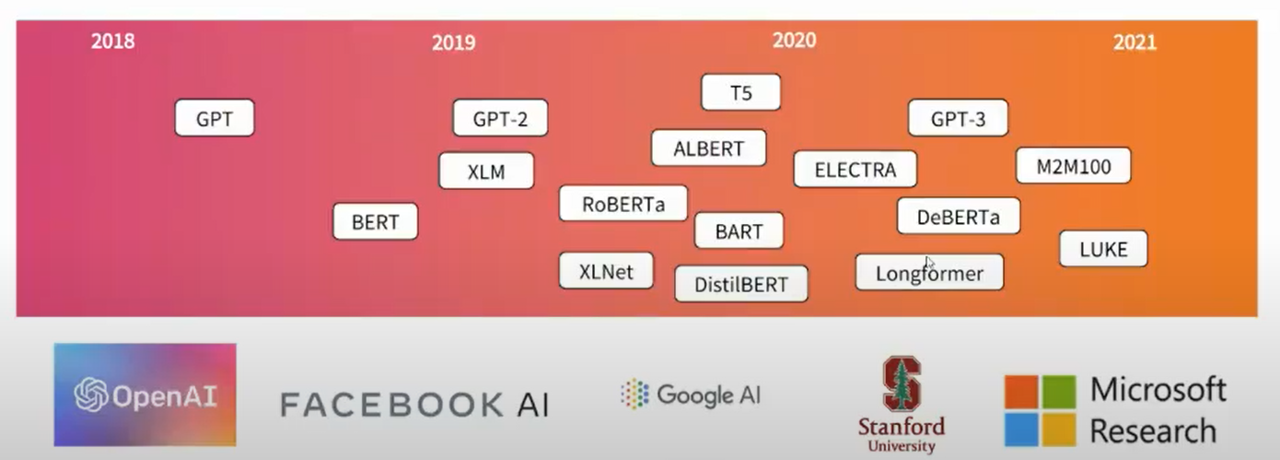
\includegraphics[width=\linewidth,keepaspectratio]{bert50}
\end{center}	

 
% {\tiny (Ref: Niels Rogge on Huggingface contributions)}
\end{frame}


%%%%%%%%%%%%%%%%%%%%%%%%%%%%%%%%%%%%%%%%%%%%%%%%%%%%%%%%%%%
\begin{frame}[fragile]\frametitle{Transformers}


\begin{itemize}
\item The Transformer  is a model that uses attention to boost the speed with which seq2seq with attention models can be trained. The biggest benefit, however, comes from how The Transformer lends itself to parallelization. We will break it apart and look at how it functions.
\item In its heart it contains an encoding component, a decoding component, and connections between them.
\end{itemize}	 

\begin{center}
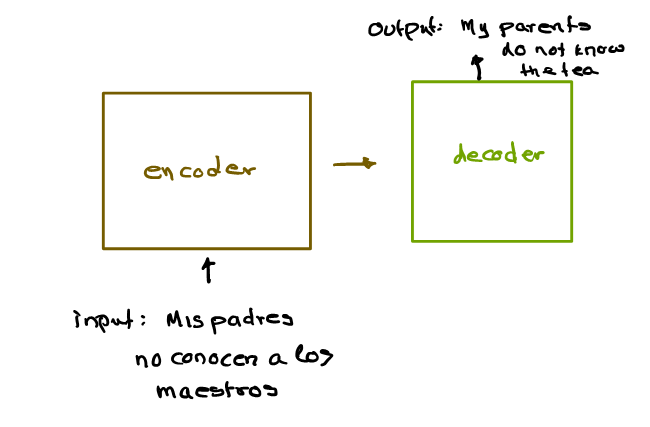
\includegraphics[width=0.6\linewidth,keepaspectratio]{bert51}
\end{center}	

\end{frame}


%%%%%%%%%%%%%%%%%%%%%%%%%%%%%%%%%%%%%%%%%%%%%%%%%%%%%%%%%%%
\begin{frame}[fragile]\frametitle{Transformers}
\begin{columns}
    \begin{column}[T]{0.5\linewidth}
      \begin{itemize}
			\item The encoding is a stack of encoders.
			\item The original paper stacks six of them on top of each other – there’s nothing magical about the number six, one can definitely experiment with other arrangements). 
			\item The decoding is a stack of decoders of the same number.
			\end{itemize}
		\end{column}
    \begin{column}[T]{0.5\linewidth}
		
			\begin{center}
			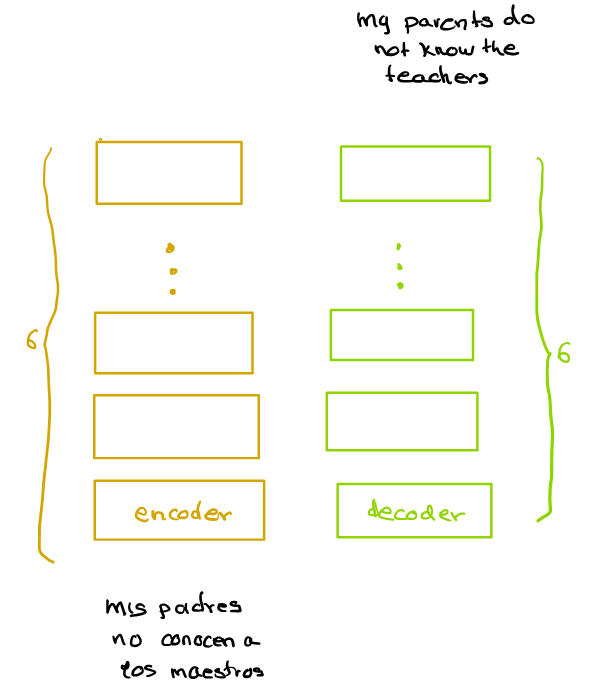
\includegraphics[width=0.8\linewidth,keepaspectratio]{bert52}
			\end{center}

    \end{column}
  \end{columns}
\end{frame}


%%%%%%%%%%%%%%%%%%%%%%%%%%%%%%%%%%%%%%%%%%%%%%%%%%%%%%%%%%%
\begin{frame}[fragile]\frametitle{Transformers}
\begin{columns}
    \begin{column}[T]{0.5\linewidth}
     The encoder’s inputs goes through a self-attention layer – a layer that helps the encoder look at other words in the input sentence as it encodes a specific word.  
		\end{column}
    \begin{column}[T]{0.5\linewidth}
		The decoder has both those layers, but between them is an attention layer that helps the decoder focus on relevant parts of the input sentence (similar what attention does in seq2seq models).
    \end{column}
  \end{columns}
	
			\begin{center}
			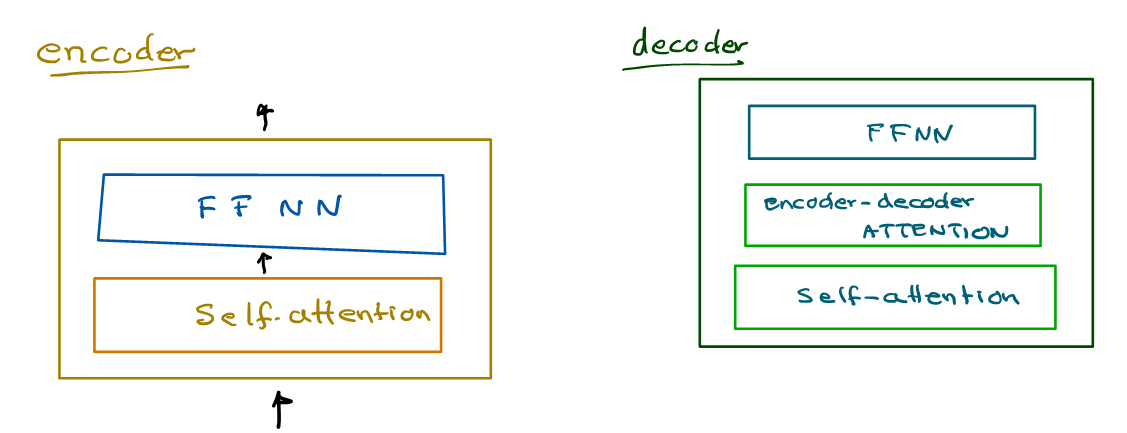
\includegraphics[width=0.8\linewidth,keepaspectratio]{bert53}
			\end{center}
			
\end{frame}

%%%%%%%%%%%%%%%%%%%%%%%%%%%%%%%%%%%%%%%%%%%%%%%%%%%%%%%%%%%
\begin{frame}[fragile]\frametitle{Transformers}
\begin{columns}
    \begin{column}[T]{0.5\linewidth}
			\begin{center}
			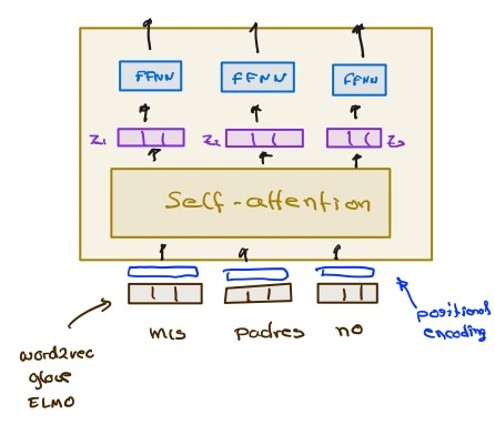
\includegraphics[width=0.8\linewidth,keepaspectratio]{bert58}
			\end{center}		
		\end{column}
    \begin{column}[T]{0.5\linewidth}
      \begin{itemize}
			\item A key property of the Transformer, which is that the word in each position flows through its own path in the encoder. There are dependencies between these paths in the self-attention layer. 
			\item The feed-forward layer does not have those dependencies, Therefore, the various paths can be executed in parallel while flowing through the feed-forward layer.
			\end{itemize}
    \end{column}
  \end{columns}
			
\end{frame}

%%%%%%%%%%%%%%%%%%%%%%%%%%%%%%%%%%%%%%%%%%%%%%%%%%%%%%%%%%%
\begin{frame}[fragile]\frametitle{Transformers}
Patrick was not late for class because {\bf he} is a responsible student

\begin{columns}
    \begin{column}[T]{0.5\linewidth}
			\begin{center}
			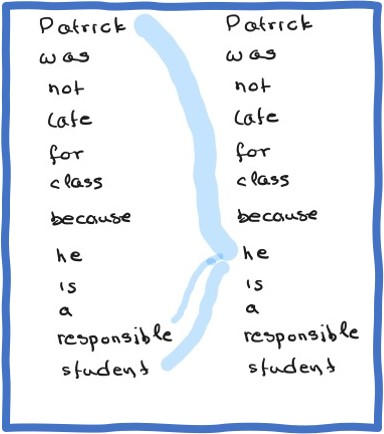
\includegraphics[width=\linewidth,keepaspectratio]{bert54}
			\end{center}		
		\end{column}
    \begin{column}[T]{0.5\linewidth}
      \begin{itemize}
			\item What does ``he'' in this sentence refer to? Is it referring to the class or to the student? It's a simple question to a human, but not as simple to an algorithm.
			\item When the model is processing the word ``he'', self-attention allows it to associate ``he'' with ``Patrick''.
			\end{itemize}
    \end{column}
  \end{columns}
			
\end{frame}

%%%%%%%%%%%%%%%%%%%%%%%%%%%%%%%%%%%%%%%%%%%%%%%%%%%%%%%%%%%
\begin{frame}[fragile]\frametitle{Transformers}
	\begin{center}
	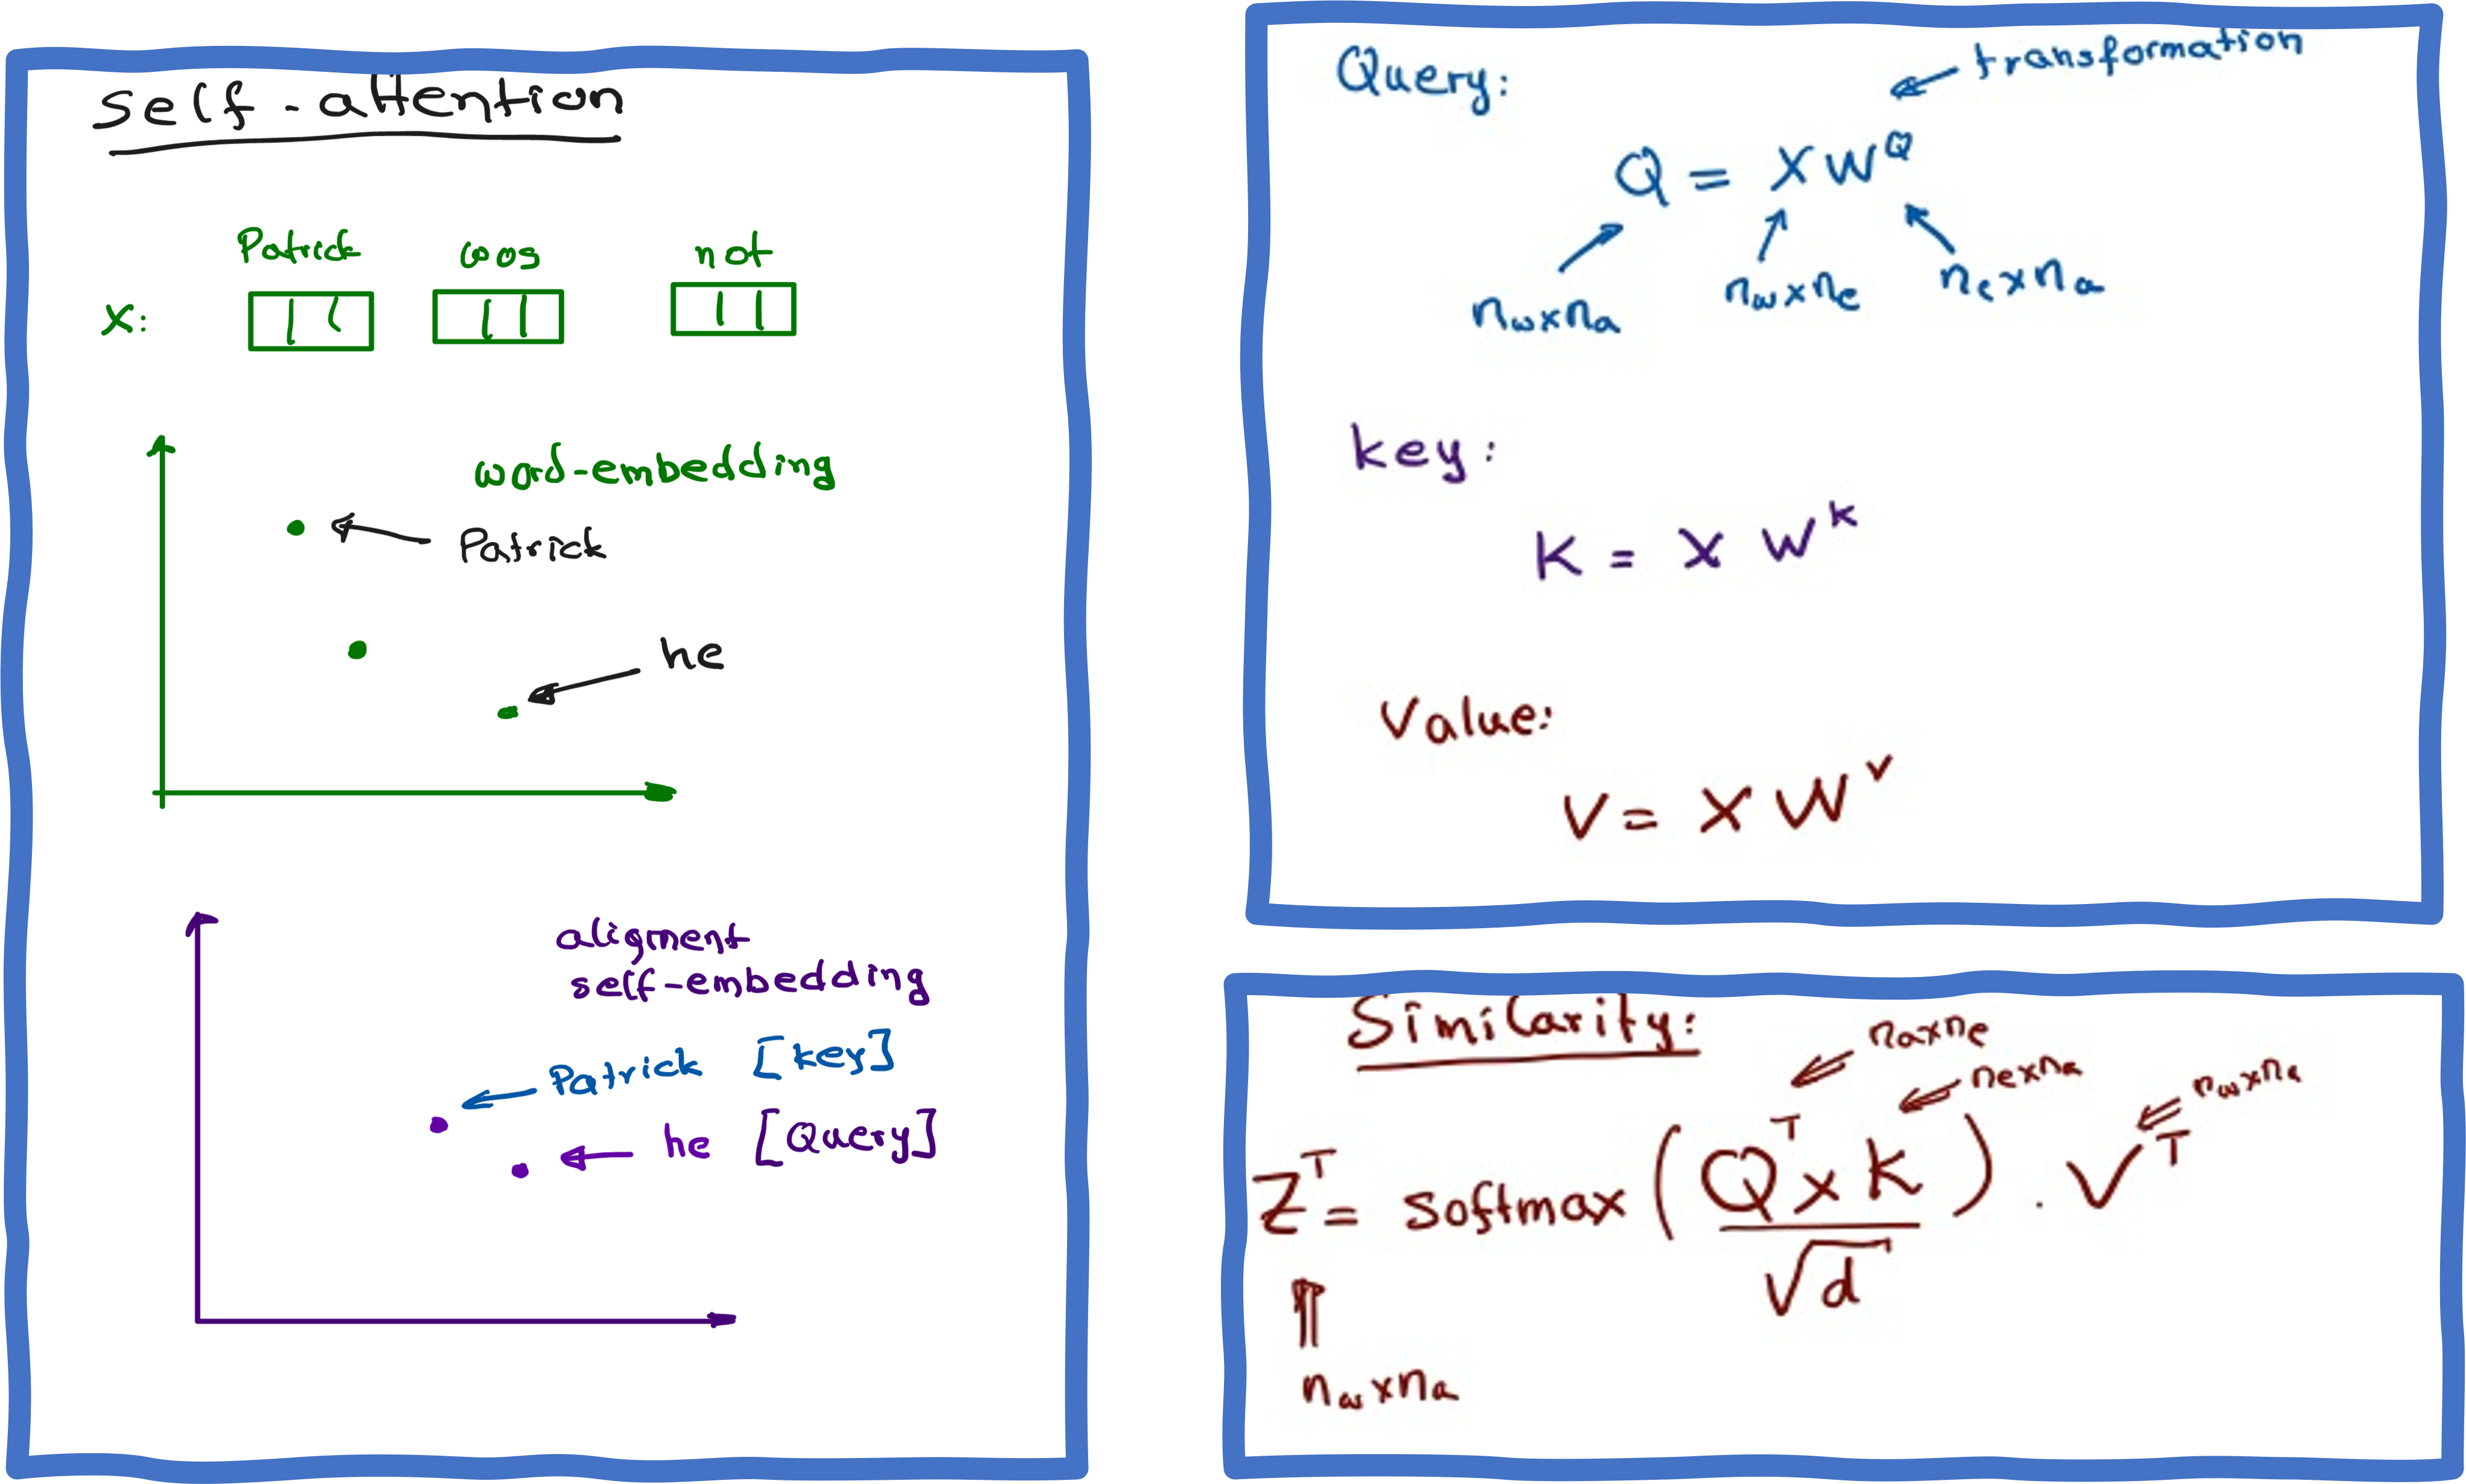
\includegraphics[width=\linewidth,keepaspectratio]{bert55}
	\end{center}	
\end{frame}

%%%%%%%%%%%%%%%%%%%%%%%%%%%%%%%%%%%%%%%%%%%%%%%%%%%%%%%%%%%
\begin{frame}[fragile]\frametitle{Transformers}

\begin{columns}
    \begin{column}[T]{0.5\linewidth}
			\begin{center}
			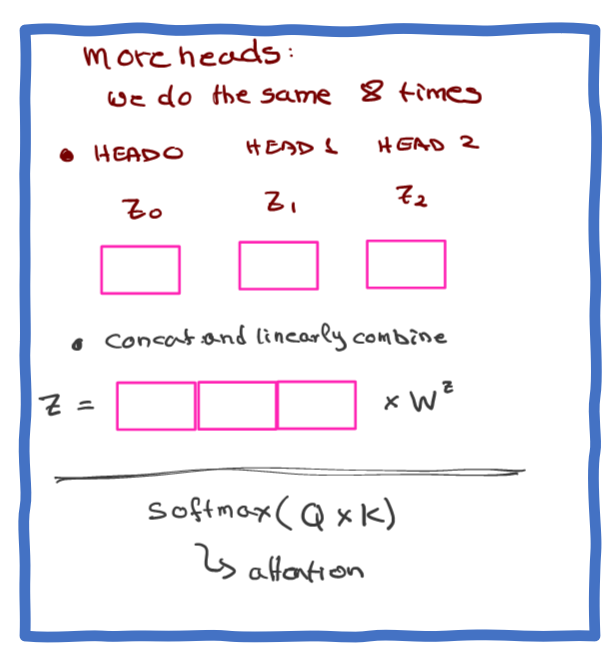
\includegraphics[width=\linewidth,keepaspectratio]{bert60}
			\end{center}		
		\end{column}
    \begin{column}[T]{0.5\linewidth}
		In the same fashion as CNN that we need more than one filter, transformers add a mechanism called ``multi-headed'' attention. This improves the performance of the attention layer in two ways:

      \begin{itemize}
			\item It expands the model's ability to focus on different positions.
			\item It gives the attention layer multiple ``representation subspaces''
			\end{itemize}
    \end{column}
  \end{columns}
			
\end{frame}

%%%%%%%%%%%%%%%%%%%%%%%%%%%%%%%%%%%%%%%%%%%%%%%%%%%%%%%%%%%
\begin{frame}[fragile]\frametitle{Transformers}

\begin{columns}
    \begin{column}[T]{0.5\linewidth}
			\begin{center}
			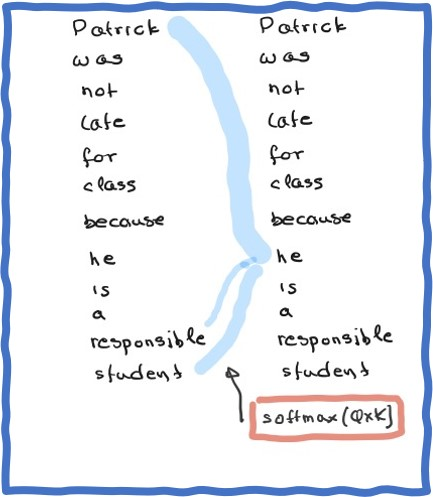
\includegraphics[width=\linewidth,keepaspectratio]{bert56}
			\end{center}		
		\end{column}
    \begin{column}[T]{0.5\linewidth}
As we encode the word ”he", one attention head is focusing most on ``Patrick'', while another is focusing on ``student'' -- in a sense, the model's representation of the word ``he'' combines the representations of both ``Patrick'' and ``stduent''.

    \end{column}
  \end{columns}
			
\end{frame}

%%%%%%%%%%%%%%%%%%%%%%%%%%%%%%%%%%%%%%%%%%%%%%%%%%%%%%%%%%%
\begin{frame}[fragile]\frametitle{Transformers}


			\begin{center}
			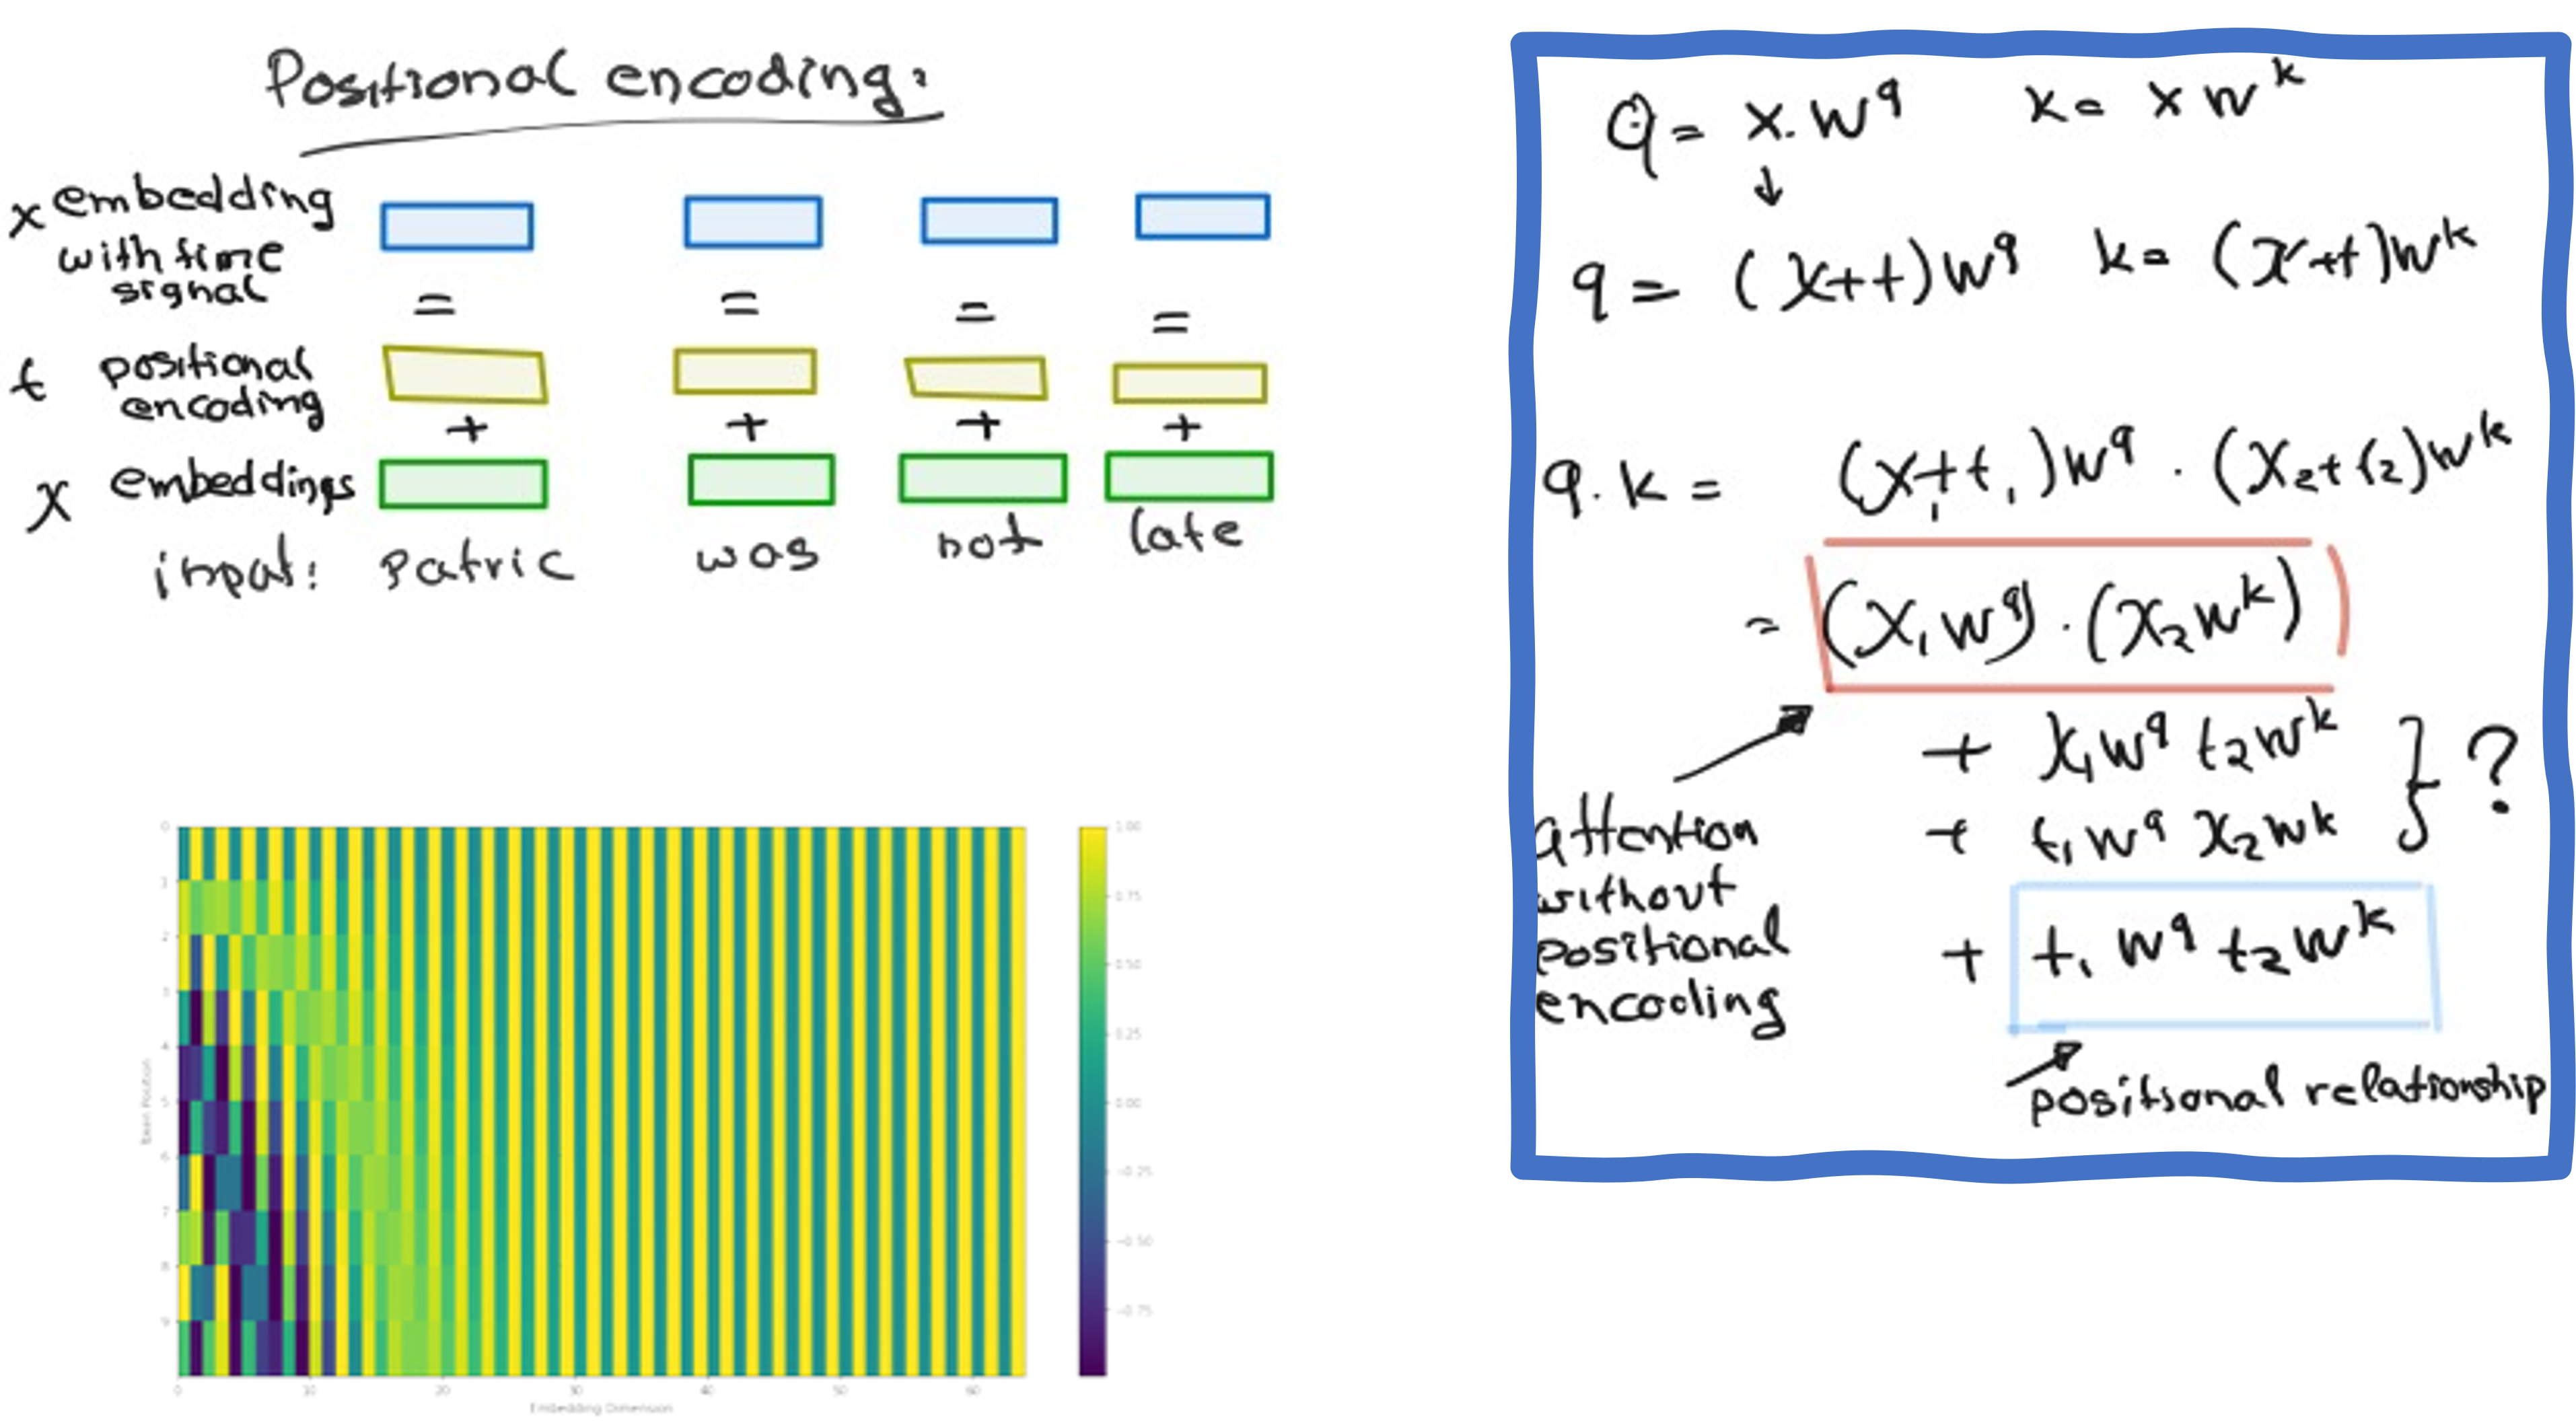
\includegraphics[width=\linewidth,keepaspectratio]{bert57}
			\end{center}		

			
\end{frame}


%%%%%%%%%%%%%%%%%%%%%%%%%%%%%%%%%%%%%%%%%%%%%%%%%%%%%%%%%%%
\begin{frame}[fragile]\frametitle{Transformers}

\begin{columns}
    \begin{column}[T]{0.5\linewidth}
			\begin{center}
			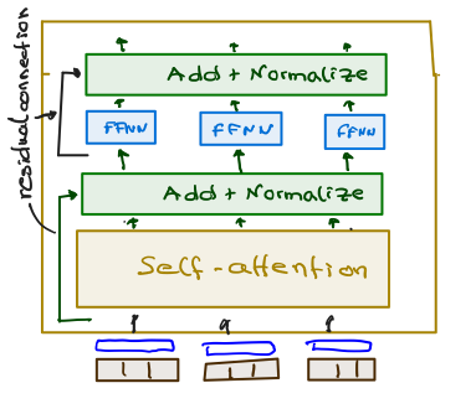
\includegraphics[width=\linewidth,keepaspectratio]{bert61}
			\end{center}		
		\end{column}
    \begin{column}[T]{0.5\linewidth}
      \begin{itemize}
			\item Details in the architecture of the encoder:
			\item Each sub-layer  in each encoder has a residual connection around it
			\item And a layer-normalization step.
			\end{itemize}
    \end{column}
  \end{columns}
			
\end{frame}

%%%%%%%%%%%%%%%%%%%%%%%%%%%%%%%%%%%%%%%%%%%%%%%%%%%%%%%%%%%
\begin{frame}[fragile]\frametitle{Transformers}


			\begin{center}
			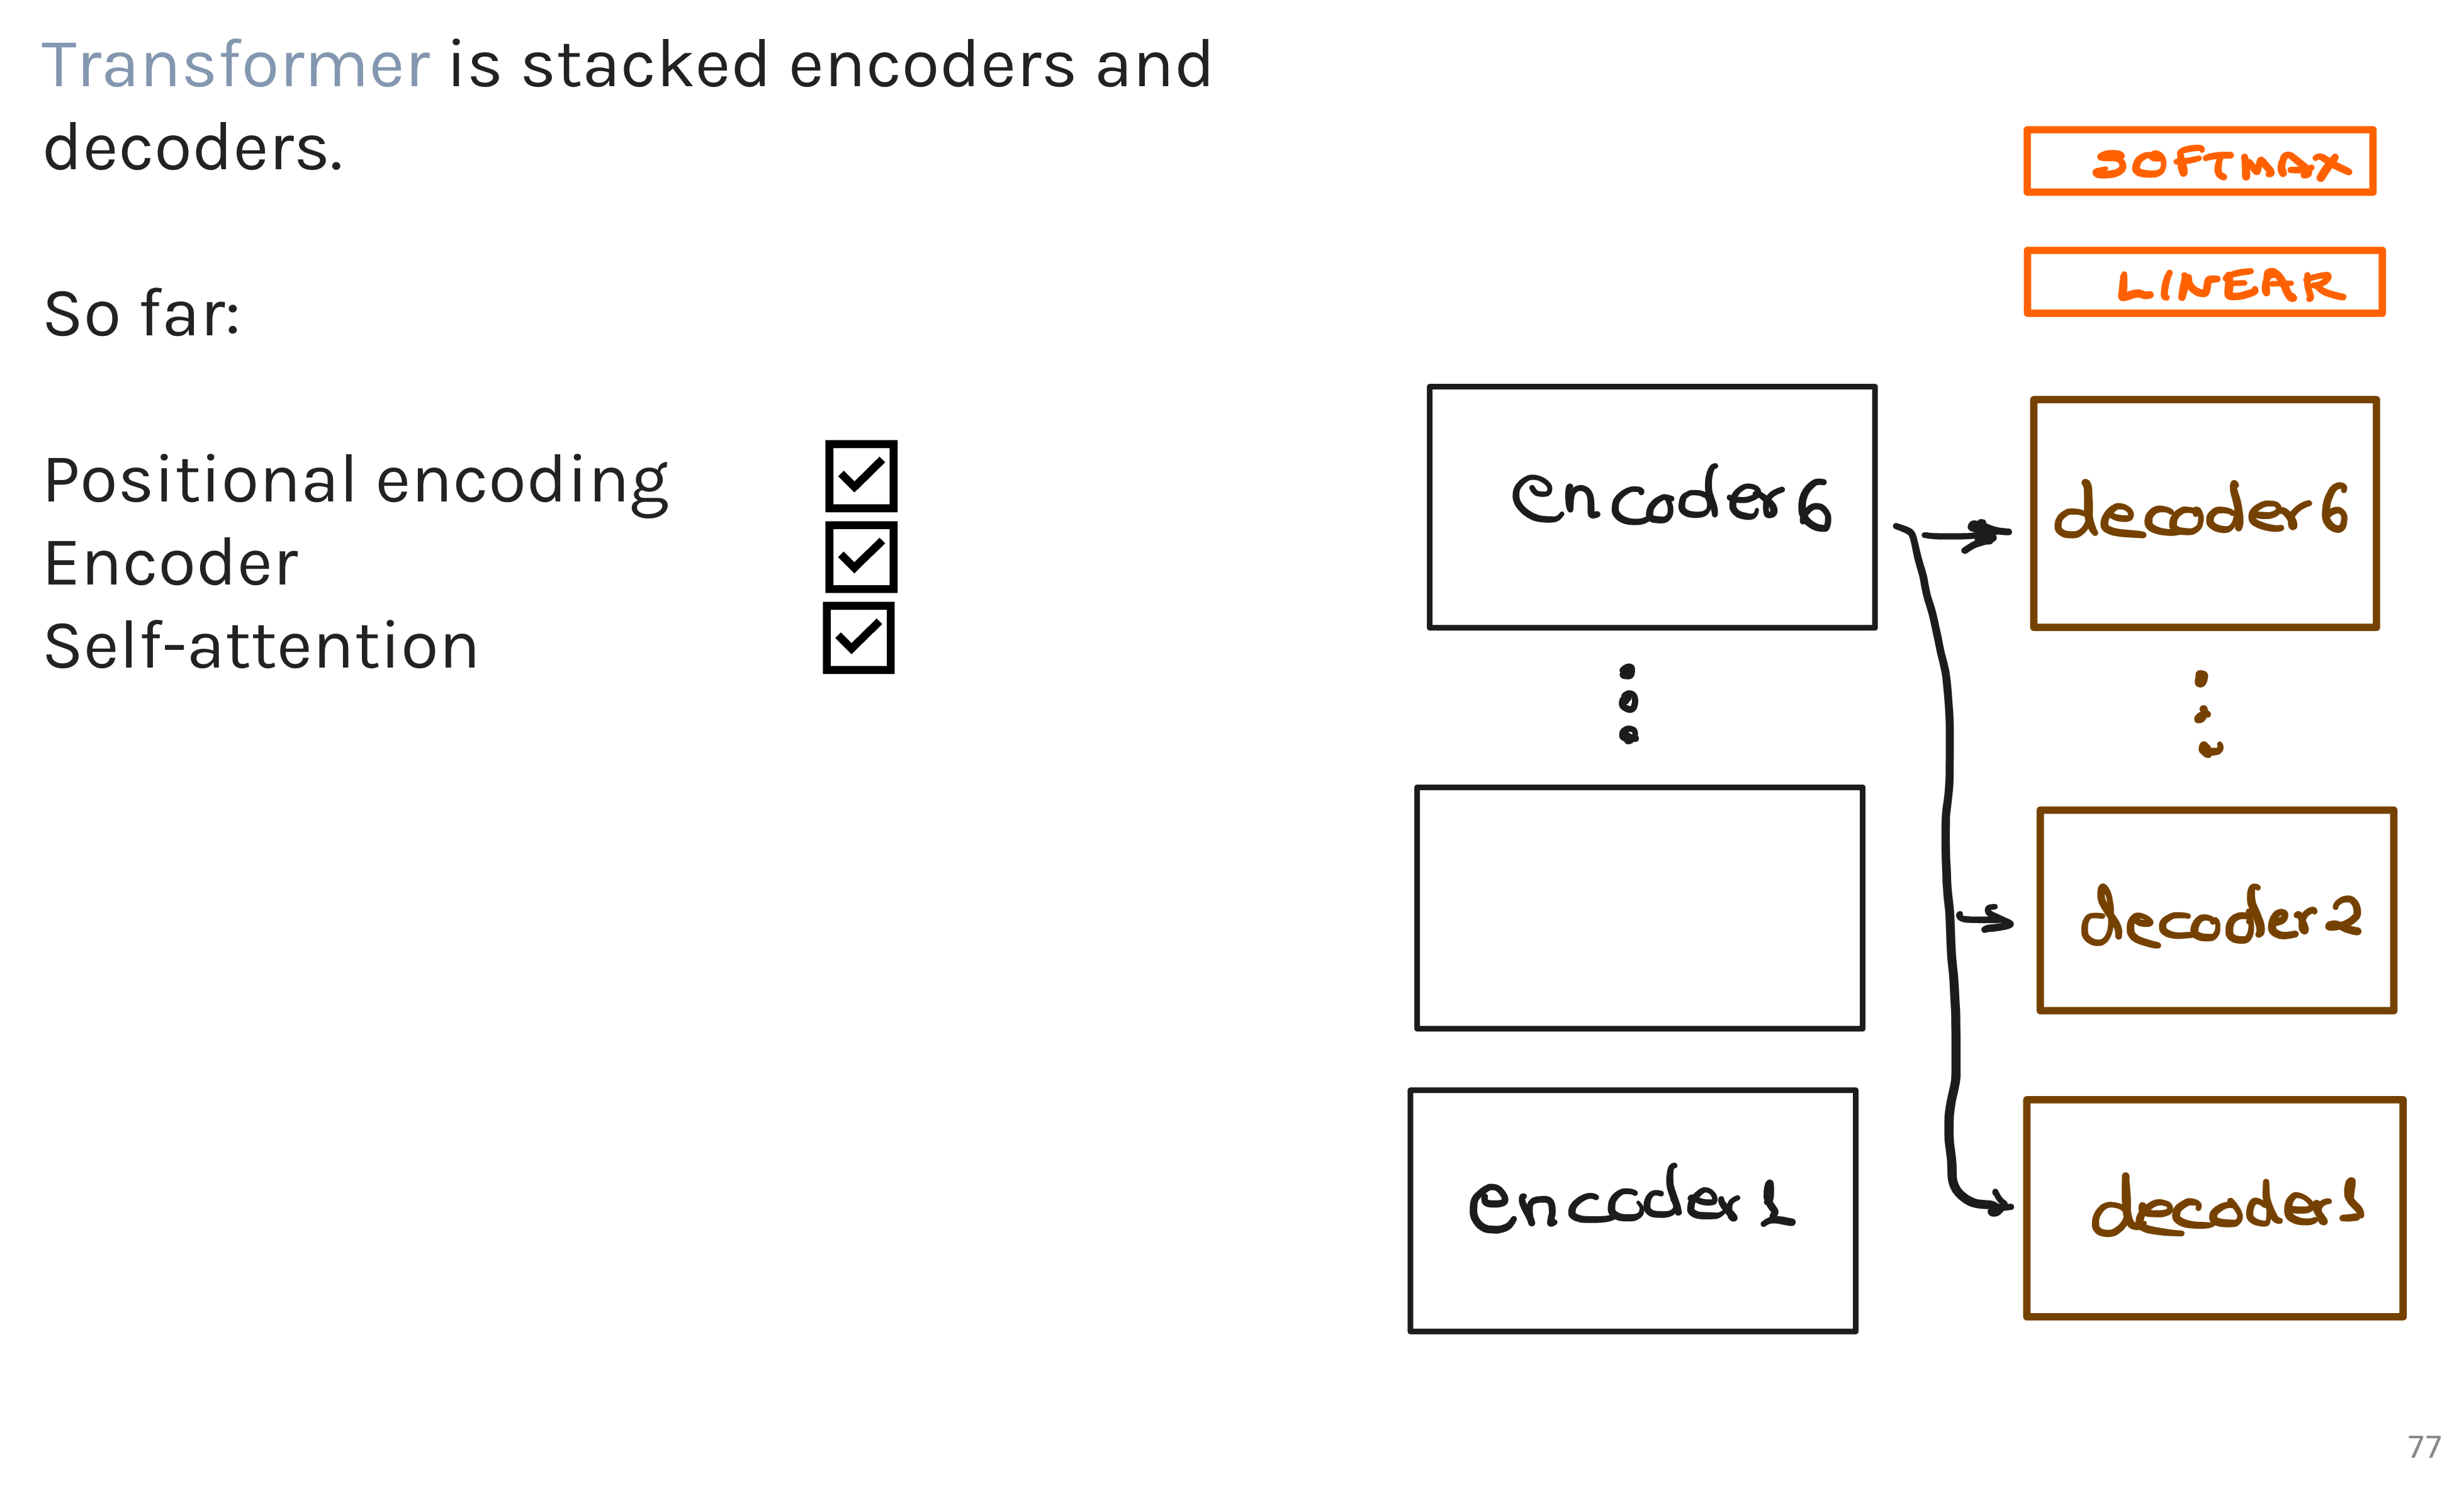
\includegraphics[width=\linewidth,keepaspectratio]{bert62}
			\end{center}		

			
\end{frame}

%%%%%%%%%%%%%%%%%%%%%%%%%%%%%%%%%%%%%%%%%%%%%%%%%%%%%%%%%%%
\begin{frame}[fragile]\frametitle{Transformers}


			\begin{center}
			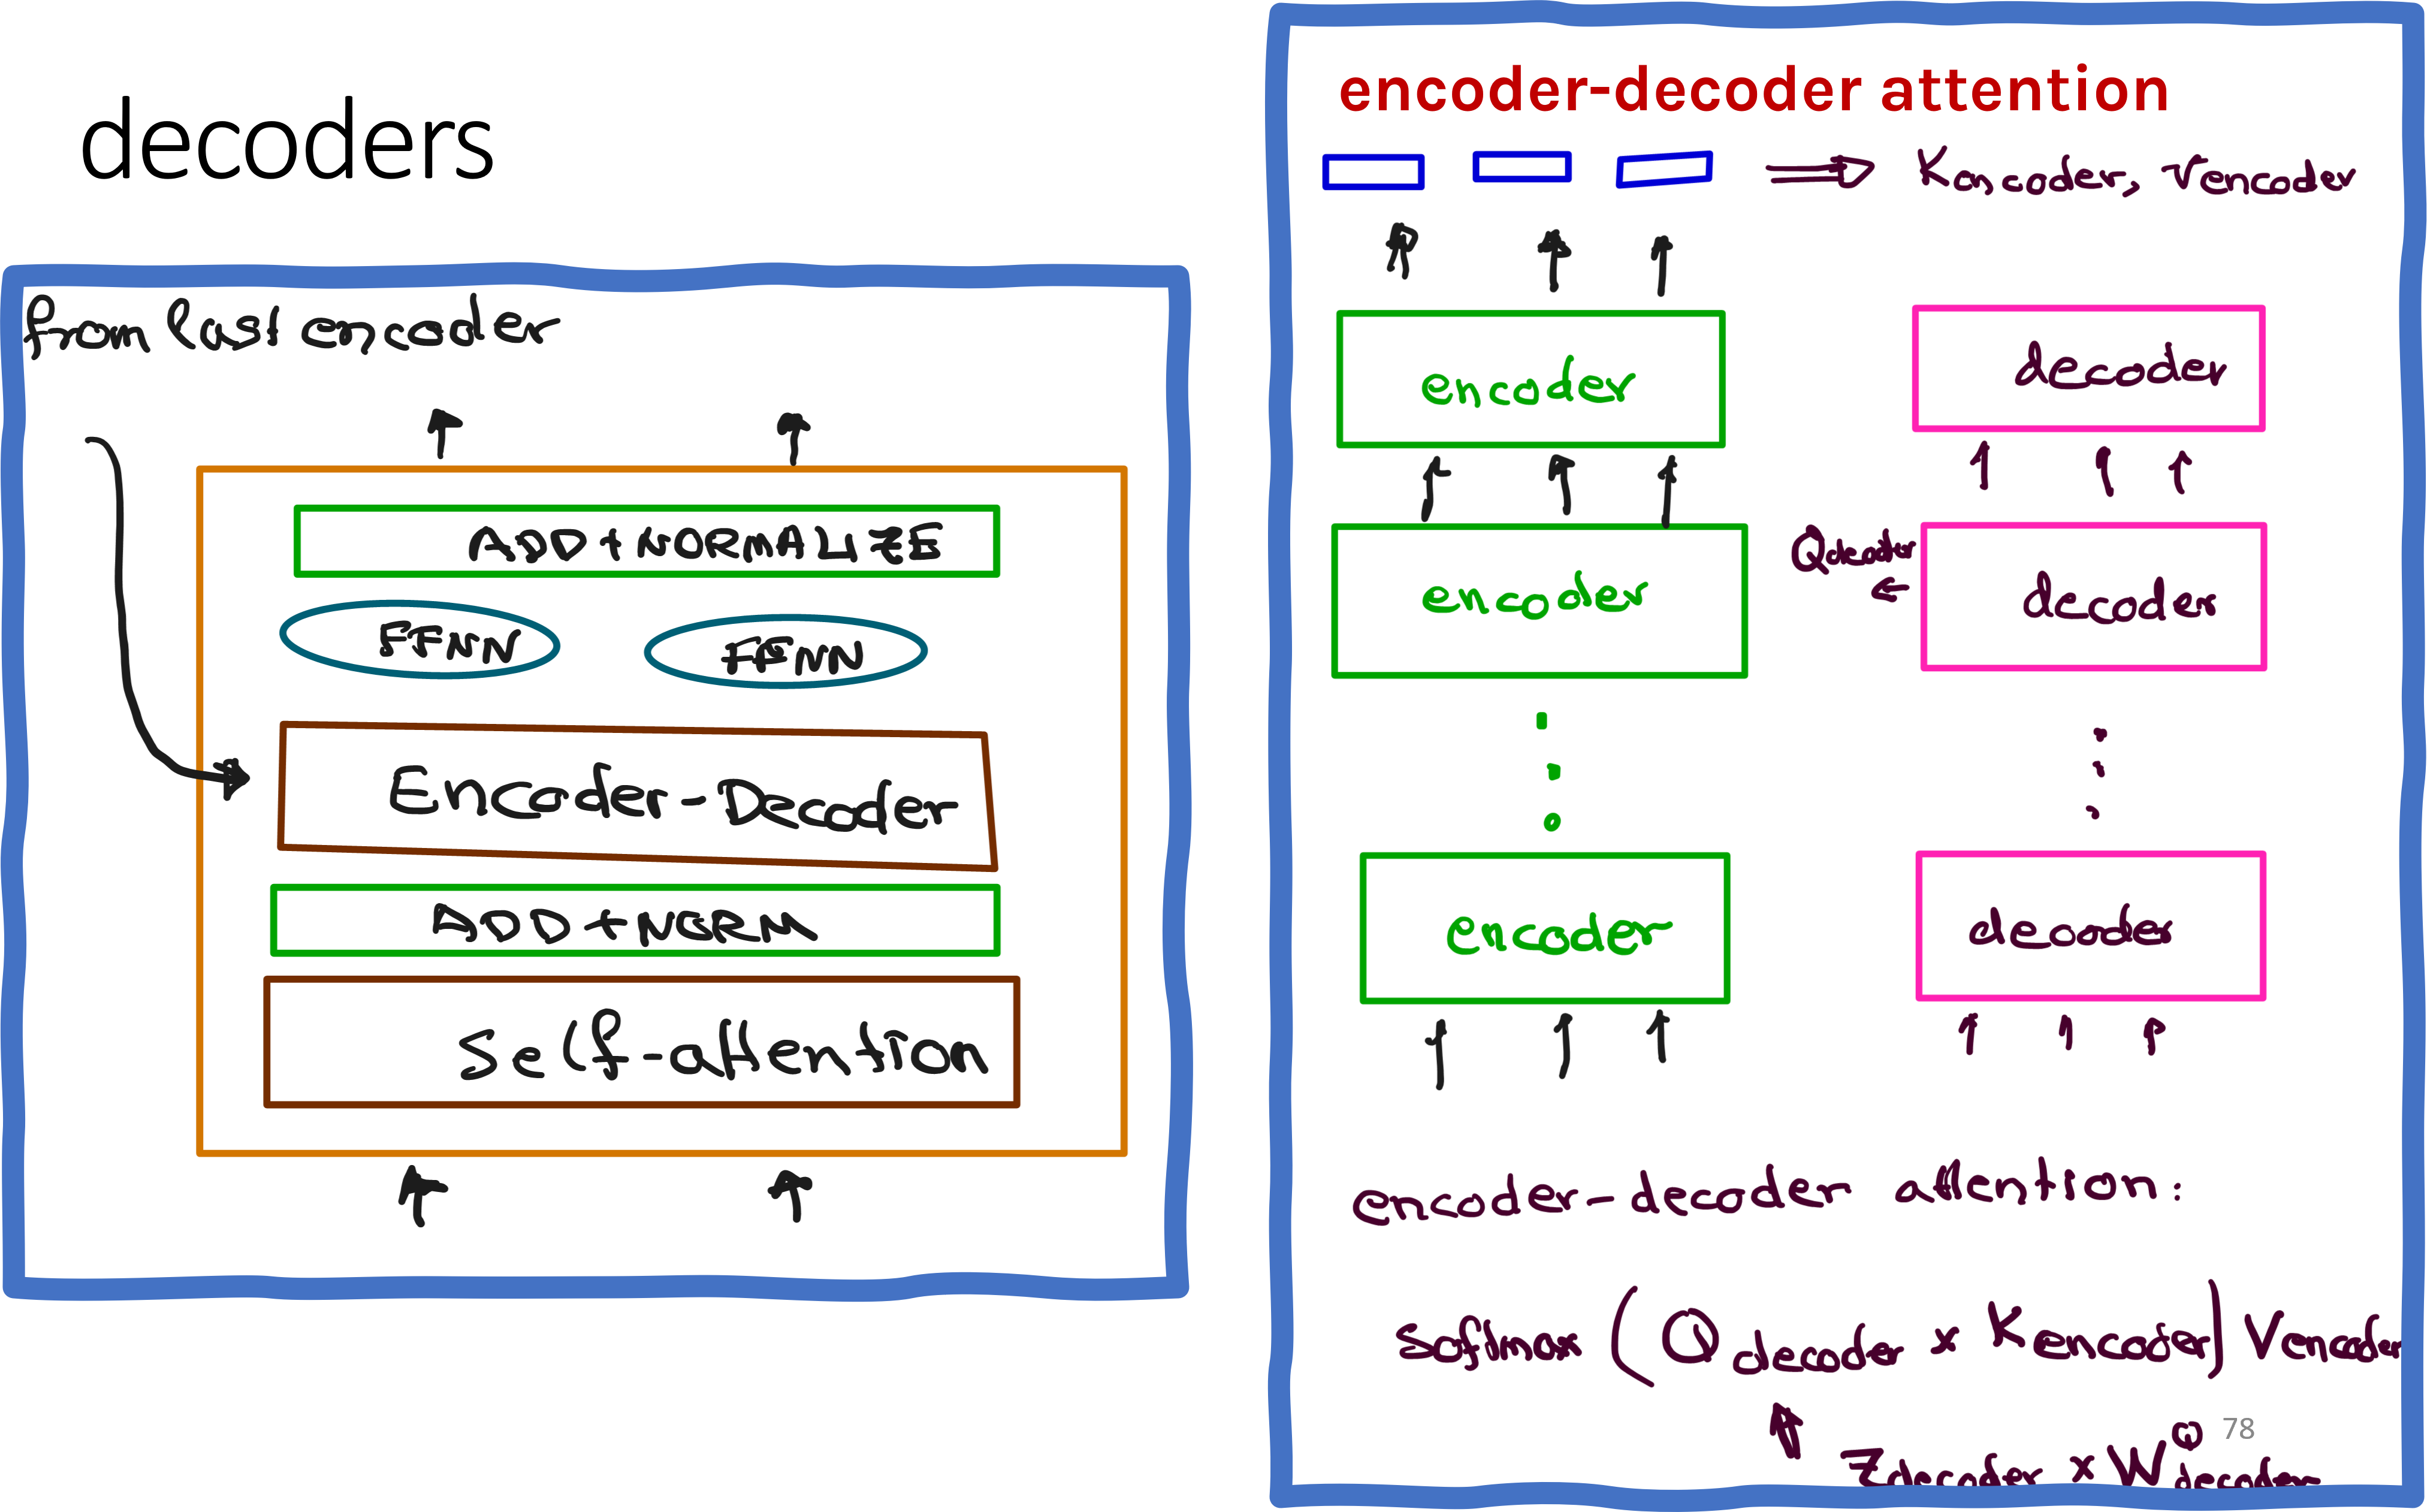
\includegraphics[width=\linewidth,keepaspectratio]{bert63}
			\end{center}		

			
\end{frame}

%%%%%%%%%%%%%%%%%%%%%%%%%%%%%%%%%%%%%%%%%%%%%%%%%%%%%%%%%%%
\begin{frame}[fragile]\frametitle{The Final Linear and Softmax Layer}


			\begin{center}
			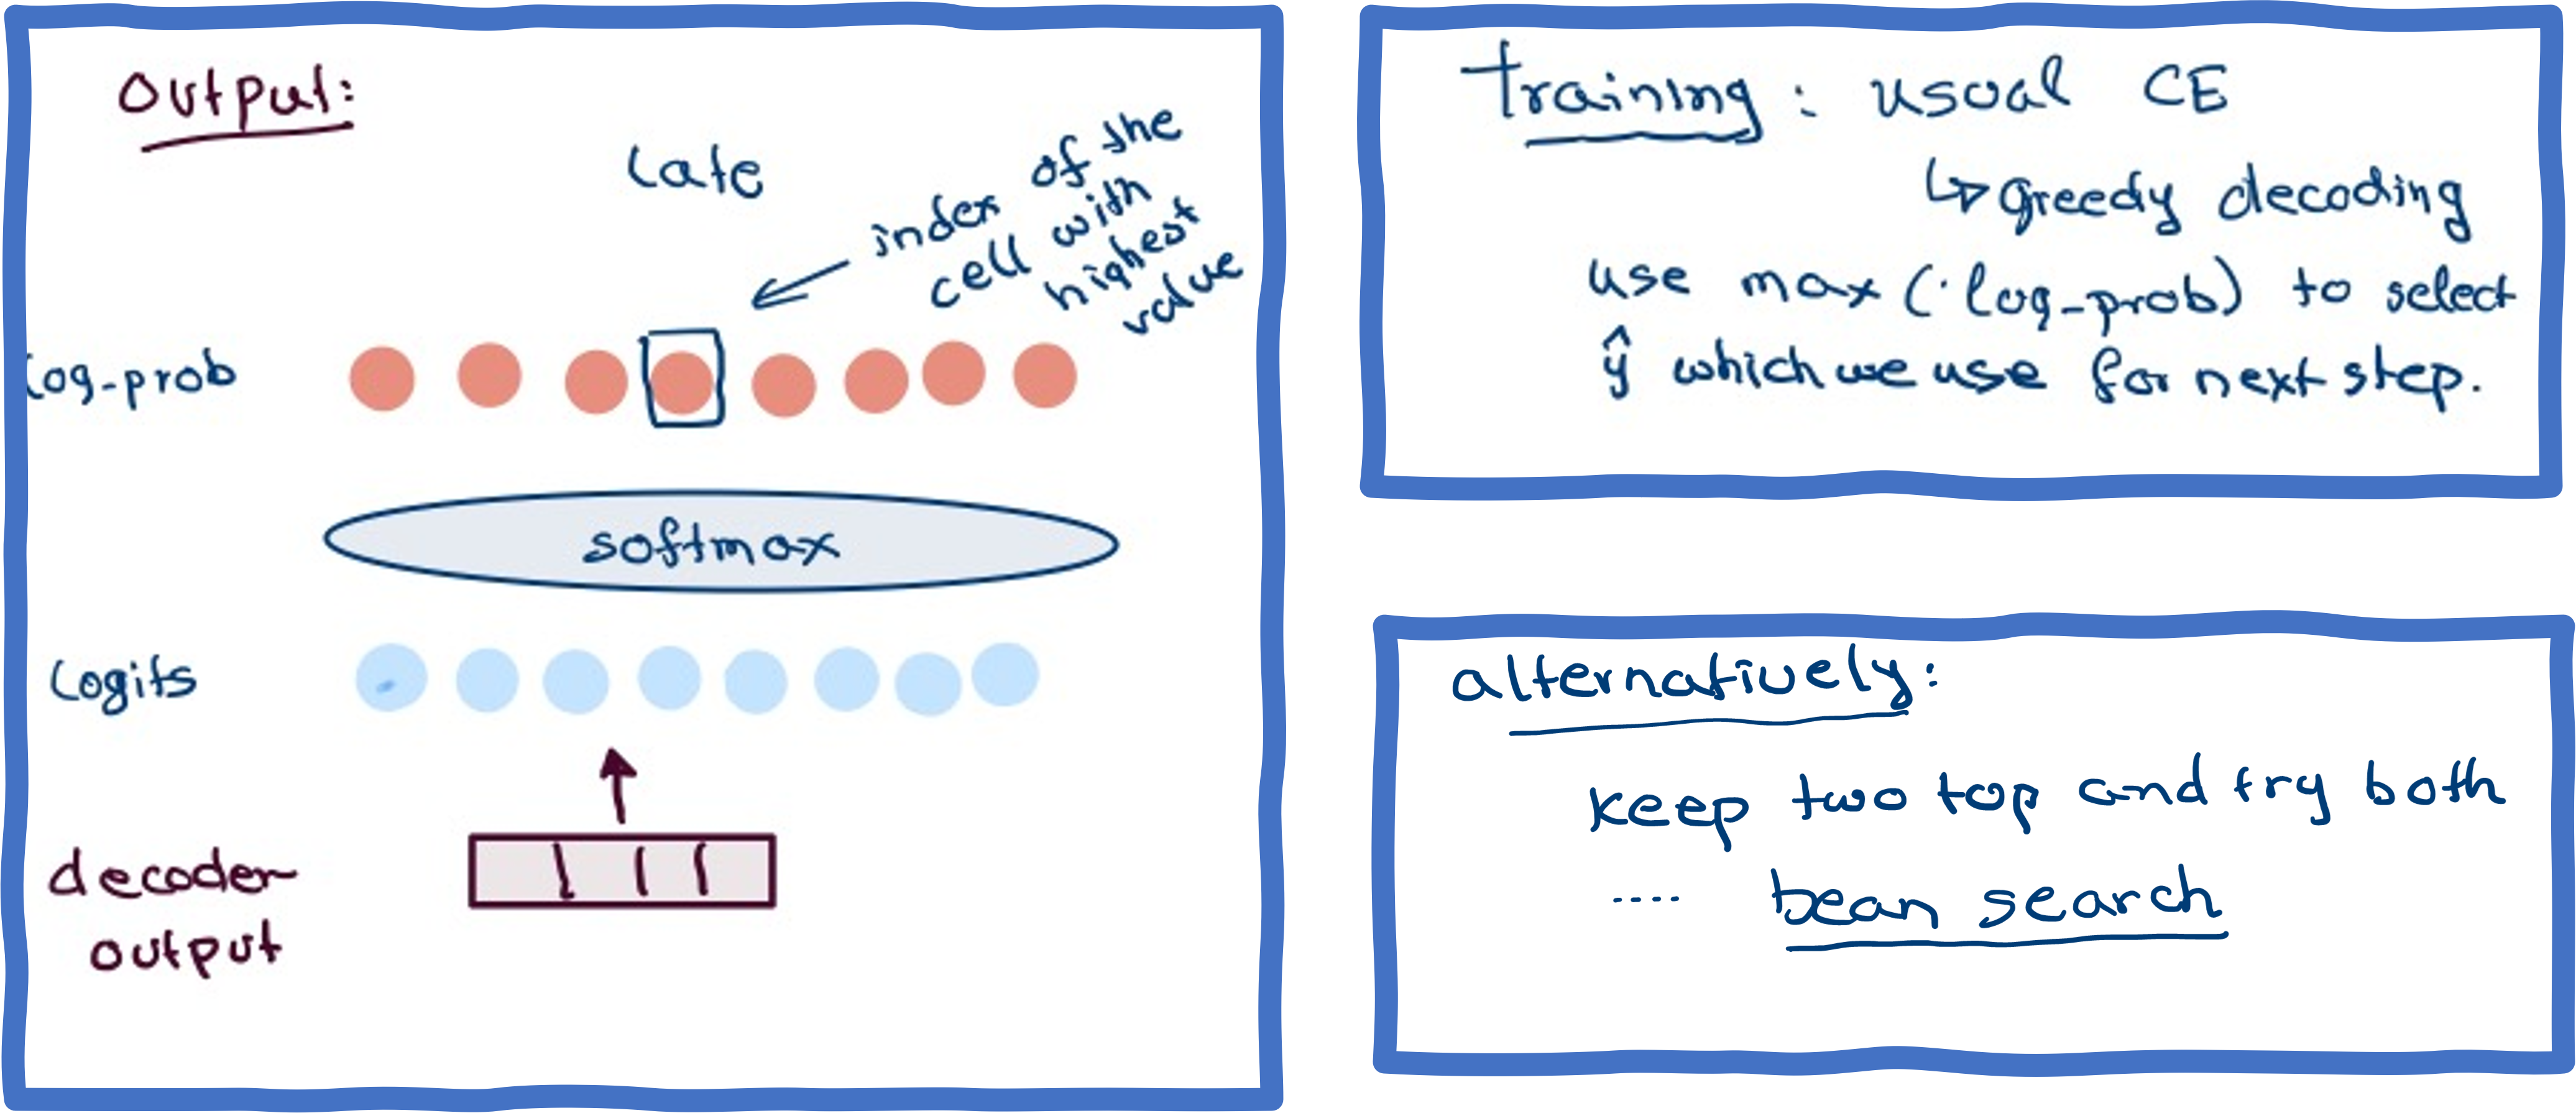
\includegraphics[width=\linewidth,keepaspectratio]{bert64}
			\end{center}		

			
\end{frame}


% %%%%%%%%%%%%%%%%%%%%%%%%%%%%%%%%%%%%%%%%%%%%%%%%%%%%%%%%%%%
% \begin{frame}[fragile]\frametitle{Transformer Overview}

% \begin{columns}
    % \begin{column}[T]{0.5\linewidth}
			% \begin{center}
			% 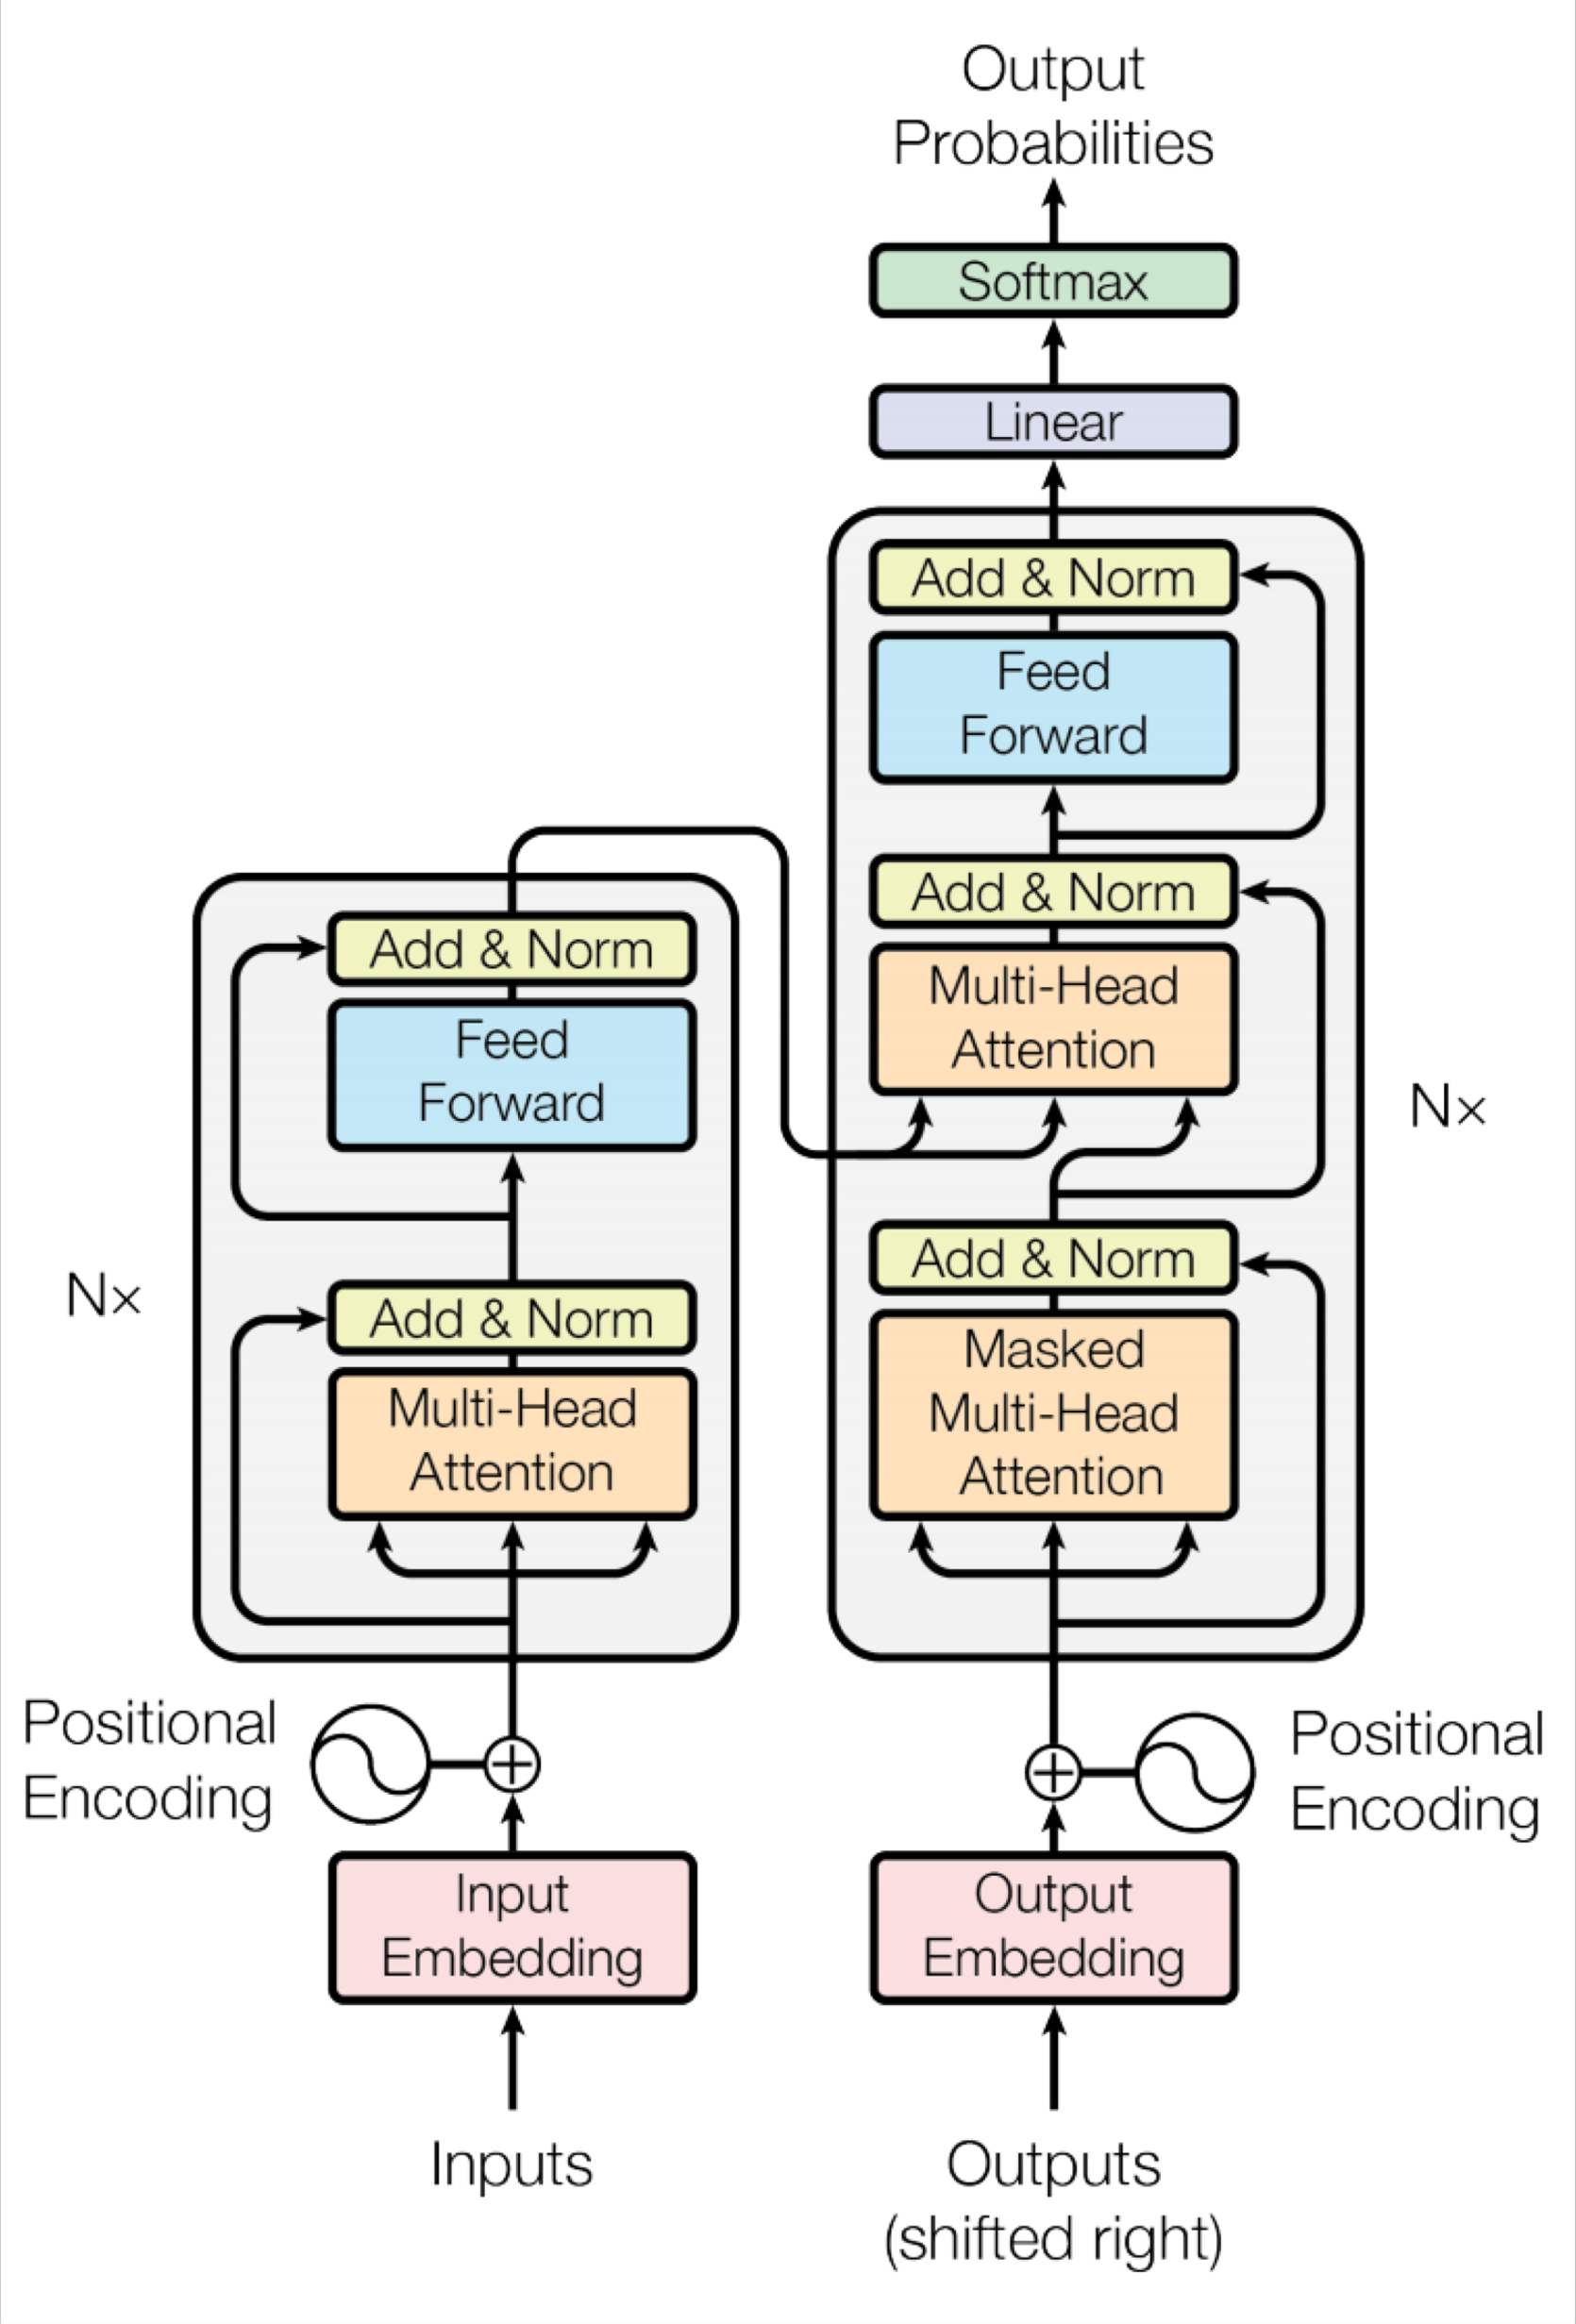
\includegraphics[width=0.8\linewidth,keepaspectratio]{bert69}
			% \end{center}		
		% \end{column}
    % \begin{column}[T]{0.5\linewidth}
		% Attention is all you need. 2017.  Aswani, Shazeer, Parmar, Uszkoreit,  Jones, Gomez, Kaiser, Polosukhin  https://arxiv.org/pdf/1706.03762.pdf 

      % \begin{itemize}
			% \item Non-recurrent sequence-to-  sequence encoder-decoder model
			% \item Task: machine translation  with parallel corpus
			% \item Predict each translated word
			% \item Final cost/error function is  standard cross-entropy error on top of a softmax classifier
			% \end{itemize}
    % \end{column}
  % \end{columns}
			
% \end{frame}

% %%%%%%%%%%%%%%%%%%%%%%%%%%%%%%%%%%%%%%%%%%%%%%%%%%%%%%%%%%%
% \begin{frame}[fragile]\frametitle{Transformer Encoder}

% \begin{columns}
    % \begin{column}[T]{0.5\linewidth}
			% \begin{center}
			% 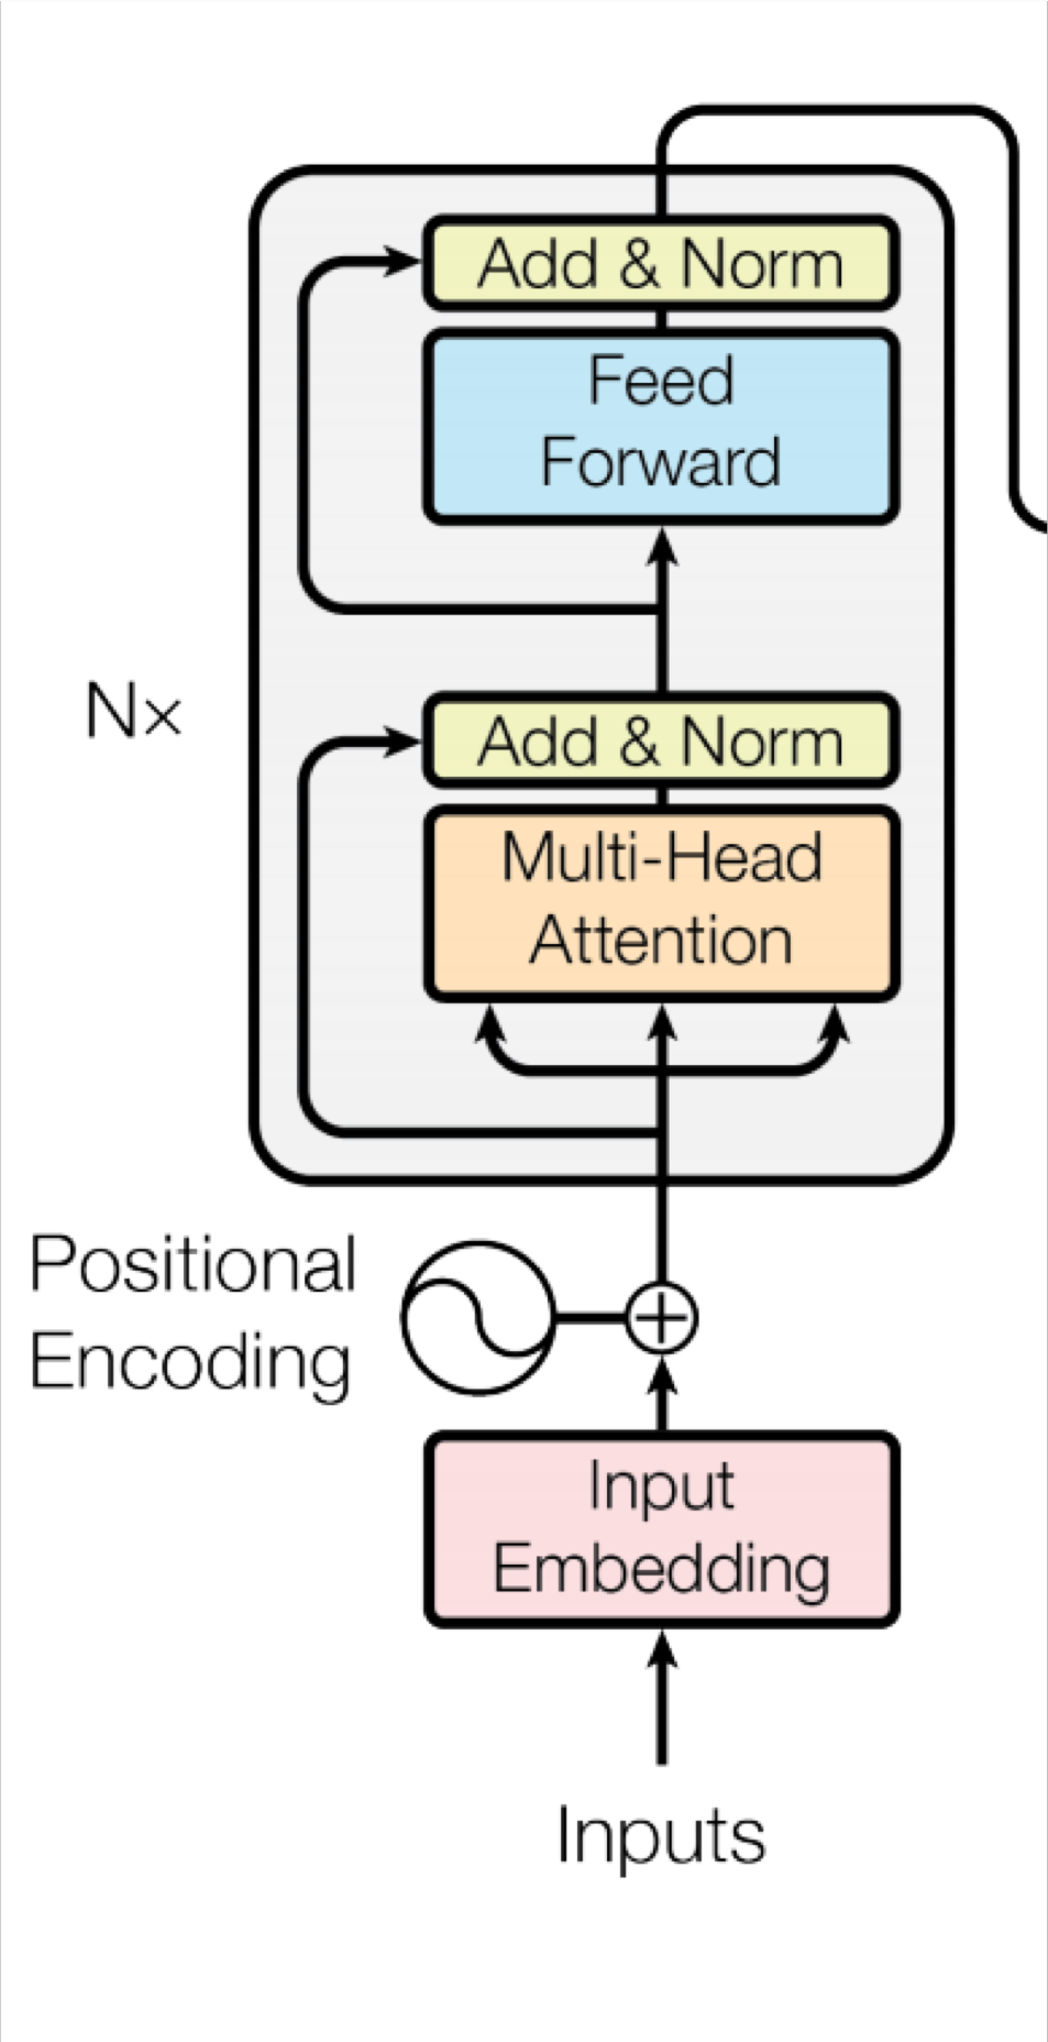
\includegraphics[width=0.6\linewidth,keepaspectratio]{bert70}
			% \end{center}		
		% \end{column}
    % \begin{column}[T]{0.5\linewidth}
      % \begin{itemize}
			% \item For encoder, at each block, we use the same Q, K and V; from the previous layer
			% \item Blocks are repeated 6 times (in vertical stack)
			% \end{itemize}
    % \end{column}
  % \end{columns}
			
% \end{frame}

% %%%%%%%%%%%%%%%%%%%%%%%%%%%%%%%%%%%%%%%%%%%%%%%%%%%%%%%%%%%
% \begin{frame}[fragile]\frametitle{Transformer Decoder}


			% \begin{center}
			% 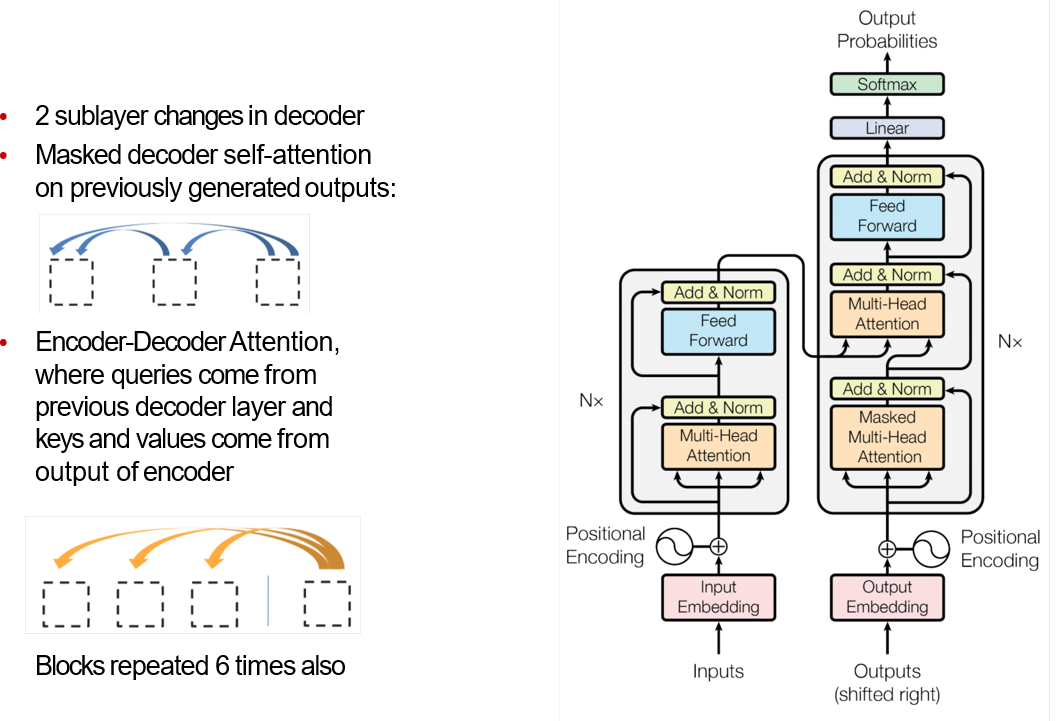
\includegraphics[width=\linewidth,keepaspectratio]{bert71}
			% \end{center}		

			
% \end{frame}

% %%%%%%%%%%%%%%%%%%%%%%%%%%%%%%%%%%%%%%%%%%%%%%%%%%%%%%%%%%%
% \begin{frame}[fragile]\frametitle{Transformer Encoder-Decoder}

			% \begin{center}
			% 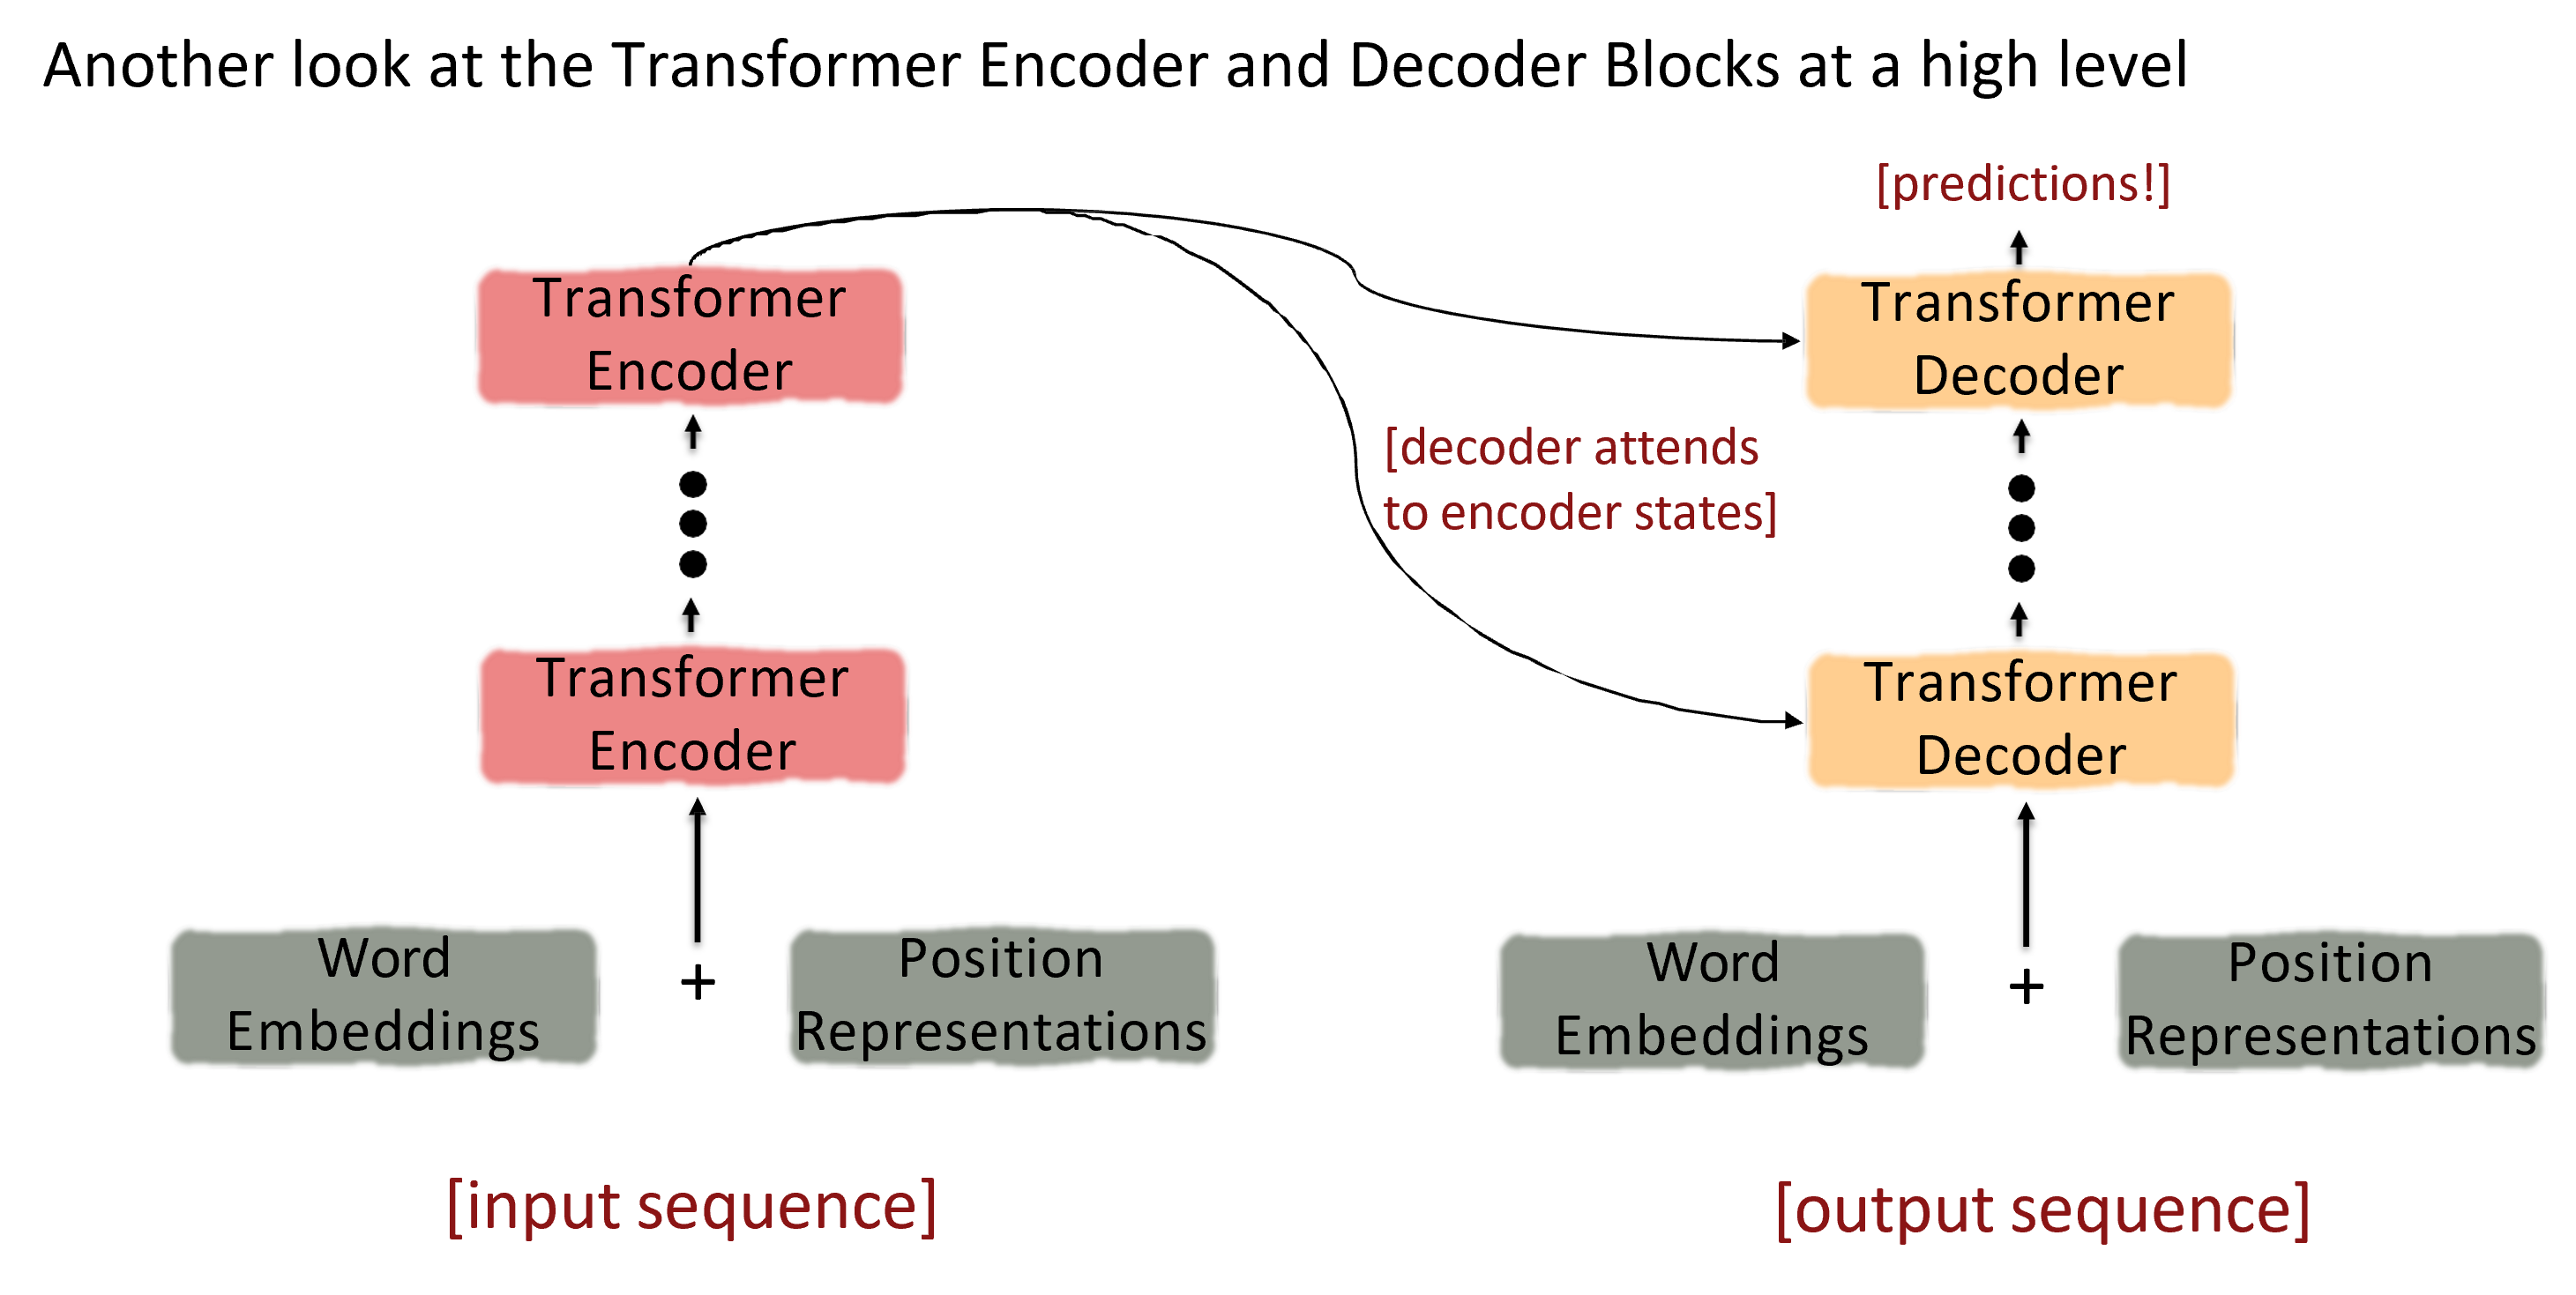
\includegraphics[width=\linewidth,keepaspectratio]{bert72}
			% \end{center}		

			
% \end{frame}

% %%%%%%%%%%%%%%%%%%%%%%%%%%%%%%%%%%%%%%%%%%%%%%%%%%%%%%%%%%%
% \begin{frame}[fragile]\frametitle{Transformer Encoder-Decoder}
% Next, let’s look at the Transformer Encoder and Decoder Blocks

% What’s left in a Transformer Encoder Block that we haven’t covered?

      % \begin{itemize}
			% \item Key-query-value attention: How do we get the $k,q,v$ vectors from a single word embedding?
			% \item Multi-headed attention: Attend to multiple places in a single layer!
			% \item Tricks to help with training!
			    % \begin{itemize}
					% \item Residual connections
					% \item Layer normalization
					% \item Scaling the dot product
					% \item These tricks don’t improve what the model is able to do; they help improve the training process
					% \end{itemize}

			% \end{itemize}
			
% \end{frame}

% %%%%%%%%%%%%%%%%%%%%%%%%%%%%%%%%%%%%%%%%%%%%%%%%%%%%%%%%%%%
% \begin{frame}[fragile]\frametitle{The Transformer Encoder: Dot-Product Attention}


      % \begin{itemize}
			% \item Inputs: a query q and a set of key-value (k-v) pairs to an output
			% \item Query, keys, values, and output are all vectors
			% \item Output is weighted sum of values, where
			% \item Weight of each value is computed by an inner product of query and corresponding key
			% \item Queries and keys have same dimensionality $d_k$ , value have $d_v$
			% \end{itemize}
			
			% \begin{center}
			% 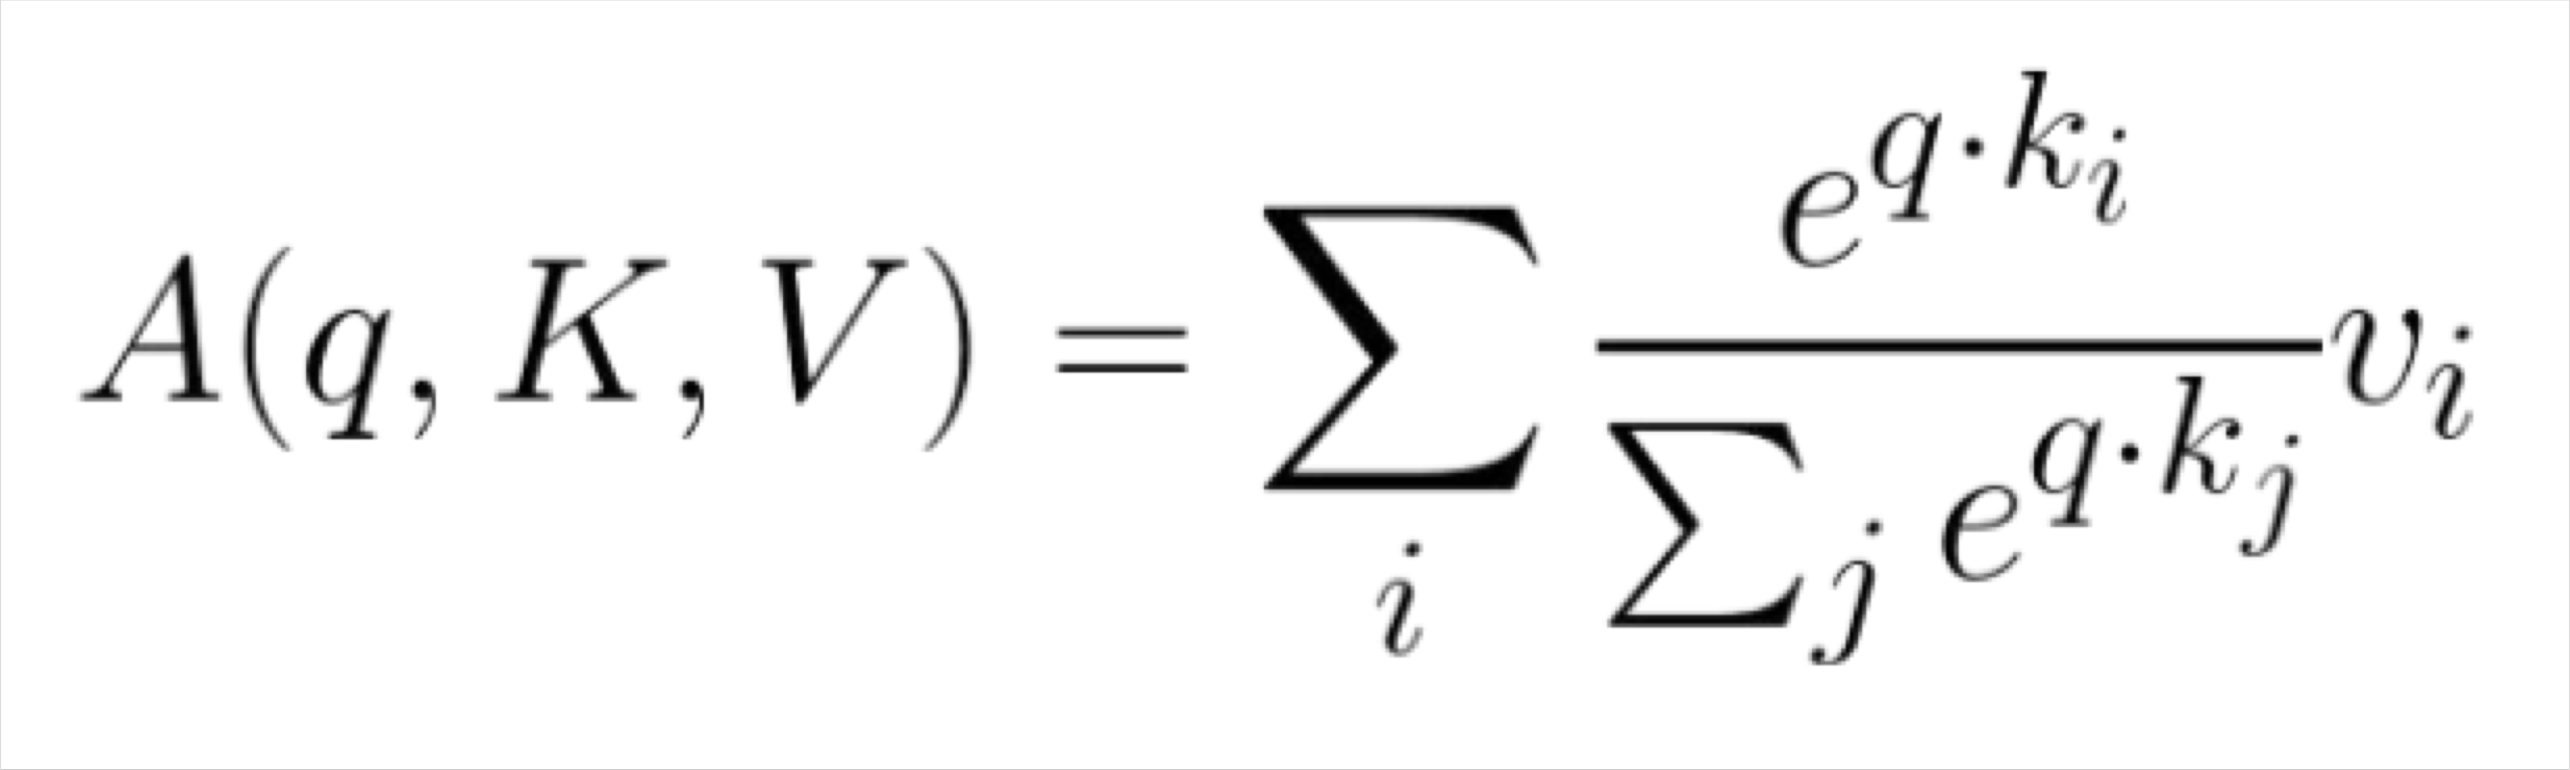
\includegraphics[width=0.4\linewidth,keepaspectratio]{bert73}
			% \end{center}		
			
			% % {\tiny (Ref: CS224n: Natural Language Processing with Deep Learning - Christopher Manning)}

% \end{frame}

% %%%%%%%%%%%%%%%%%%%%%%%%%%%%%%%%%%%%%%%%%%%%%%%%%%%%%%%%%%%
% \begin{frame}[fragile]\frametitle{The Transformer Encoder: Dot-Product Attention: Matrix notation}


      % \begin{itemize}
			% \item Inputs: a query q and a set of key-value (k-v) pairs to an output
			% \item Query, keys, values, and output are all vectors
			% \item Output is weighted sum of values, where
			% \item Weight of each value is computed by an inner product of query and corresponding key
			% \item Queries and keys have same dimensionality $d_k$ , value have $d_v$
			% \end{itemize}
			
			% \begin{center}
			% 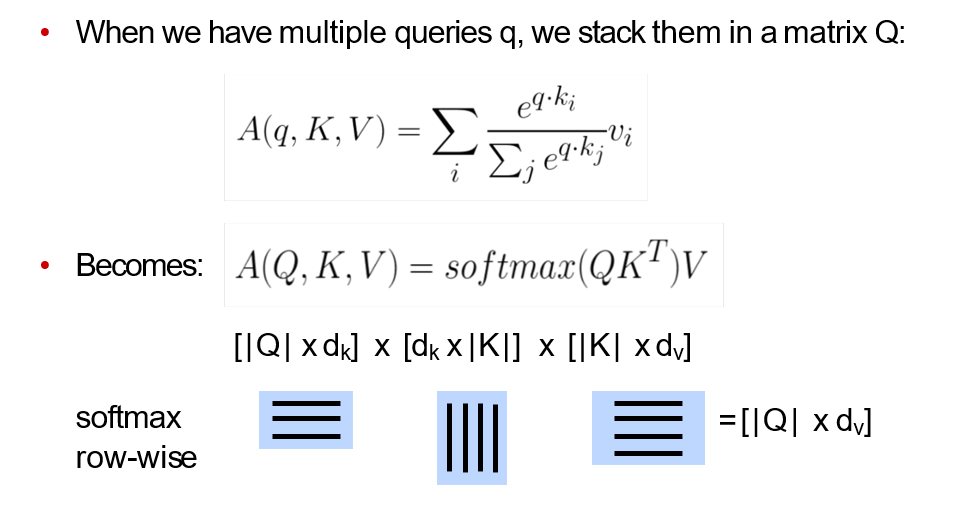
\includegraphics[width=0.8\linewidth,keepaspectratio]{bert74}
			% \end{center}		
			
			% % {\tiny (Ref: CS224n: Natural Language Processing with Deep Learning - Christopher Manning)}

% \end{frame}

% %%%%%%%%%%%%%%%%%%%%%%%%%%%%%%%%%%%%%%%%%%%%%%%%%%%%%%%%%%%
% \begin{frame}[fragile]\frametitle{The Transformer Encoder: Key-Query-Value Attention}

			
			% \begin{center}
			% 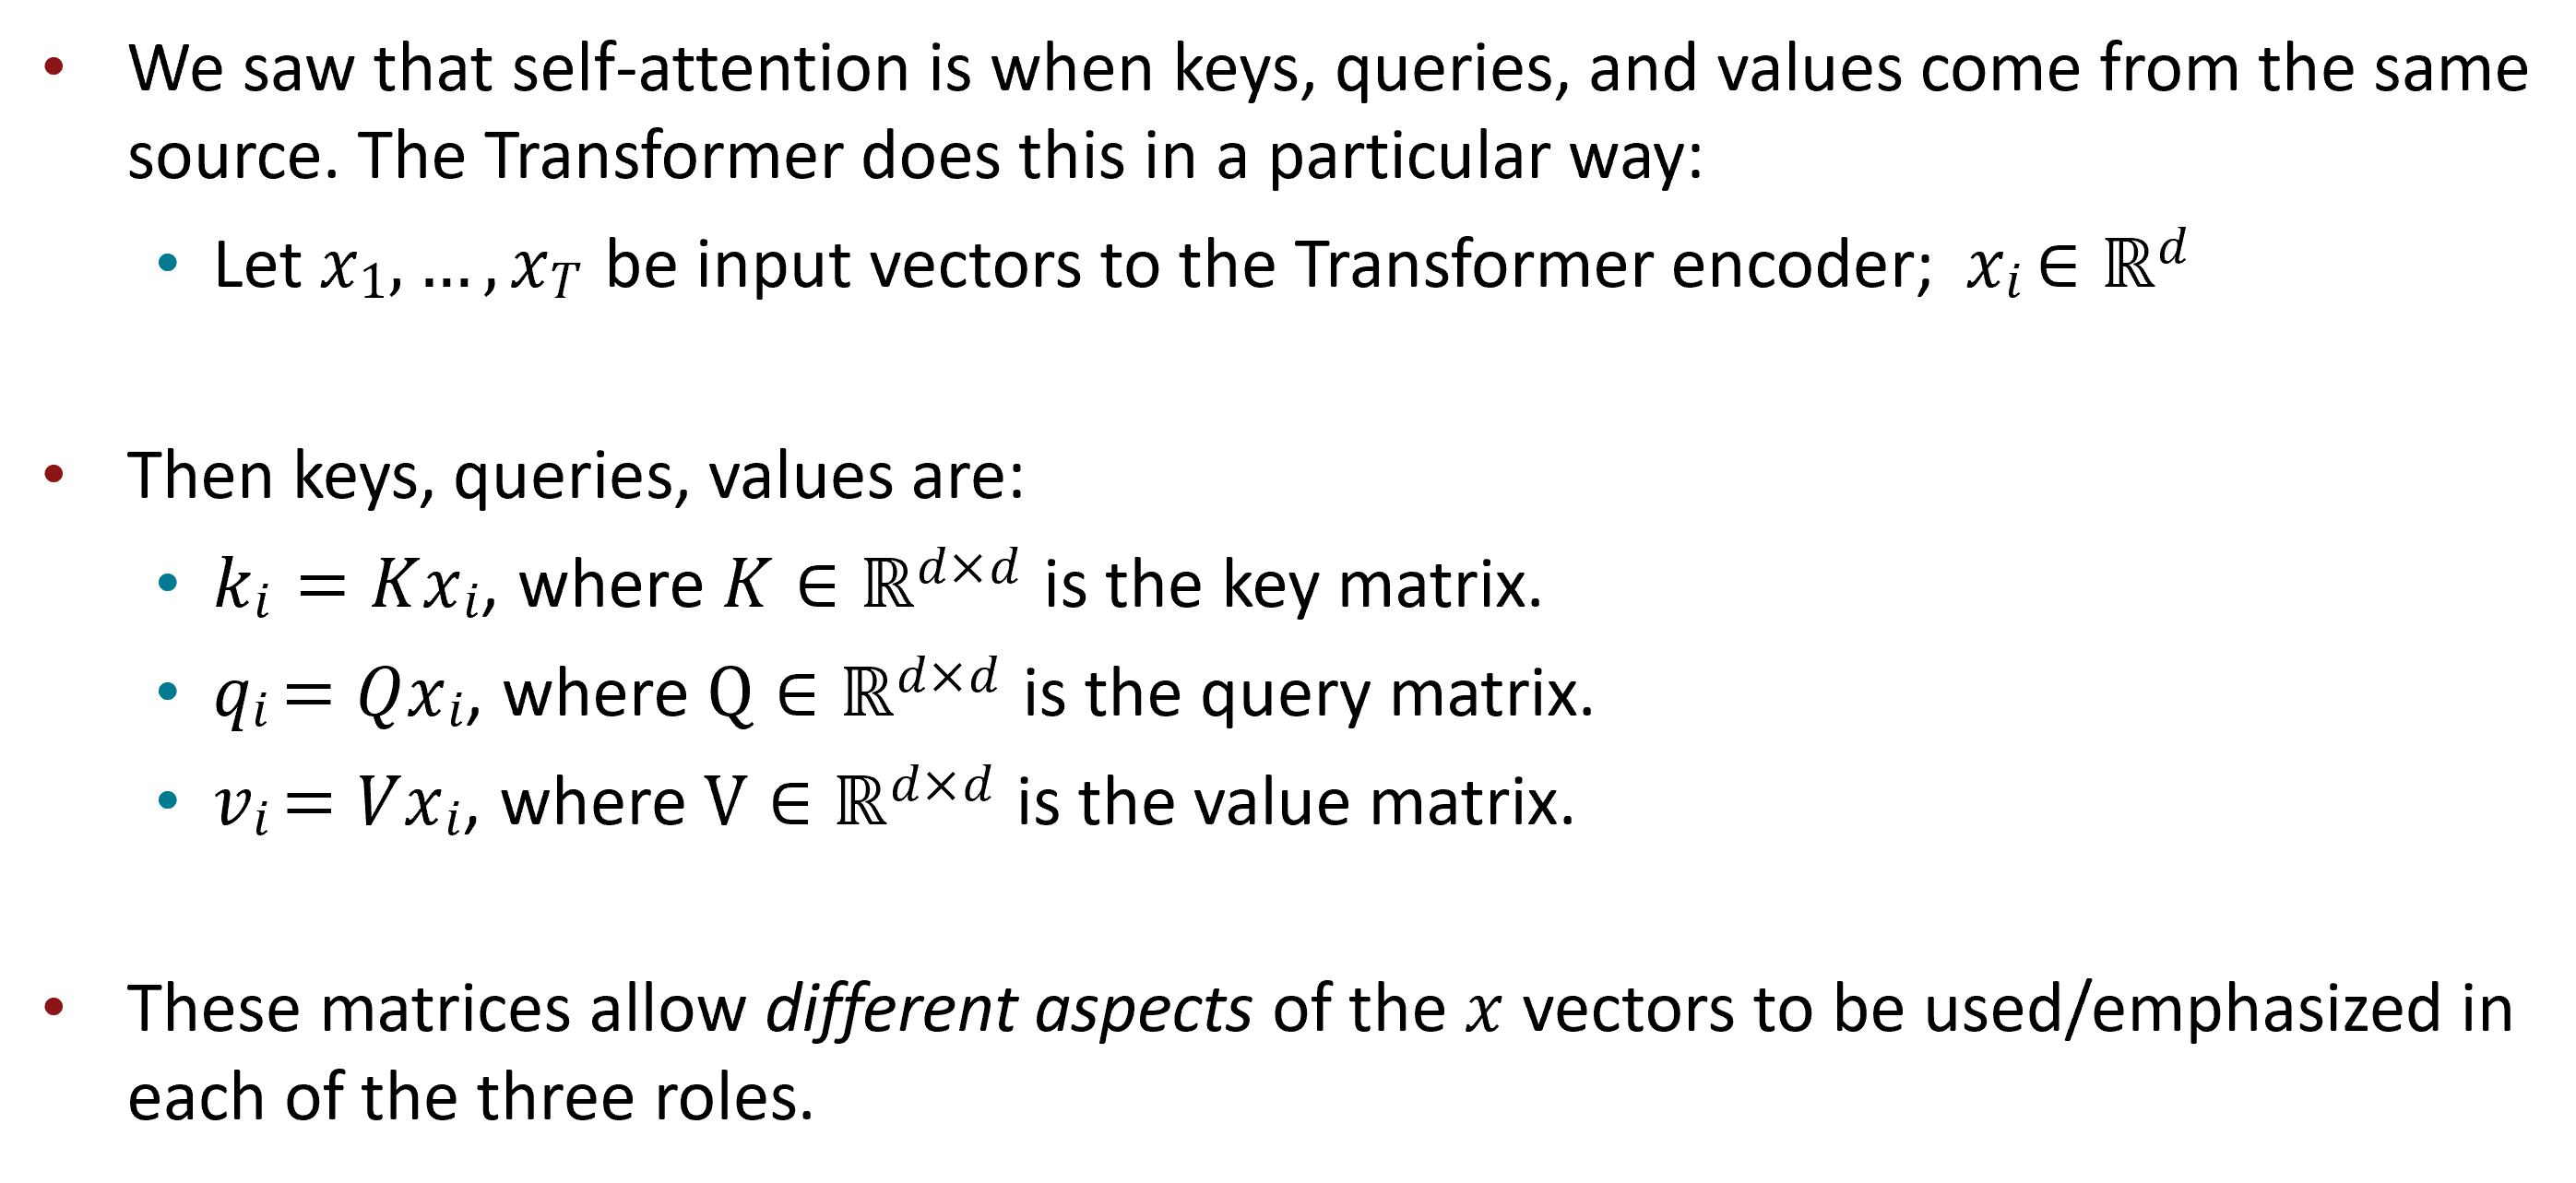
\includegraphics[width=\linewidth,keepaspectratio]{bert75}
			% \end{center}		
			
% % {\tiny (Ref: Language \& Machine Learning - John Hewitt)}

% \end{frame}

% %%%%%%%%%%%%%%%%%%%%%%%%%%%%%%%%%%%%%%%%%%%%%%%%%%%%%%%%%%%
% \begin{frame}[fragile]\frametitle{The Transformer Encoder: Key-Query-Value Attention}

			
			% \begin{center}
			% 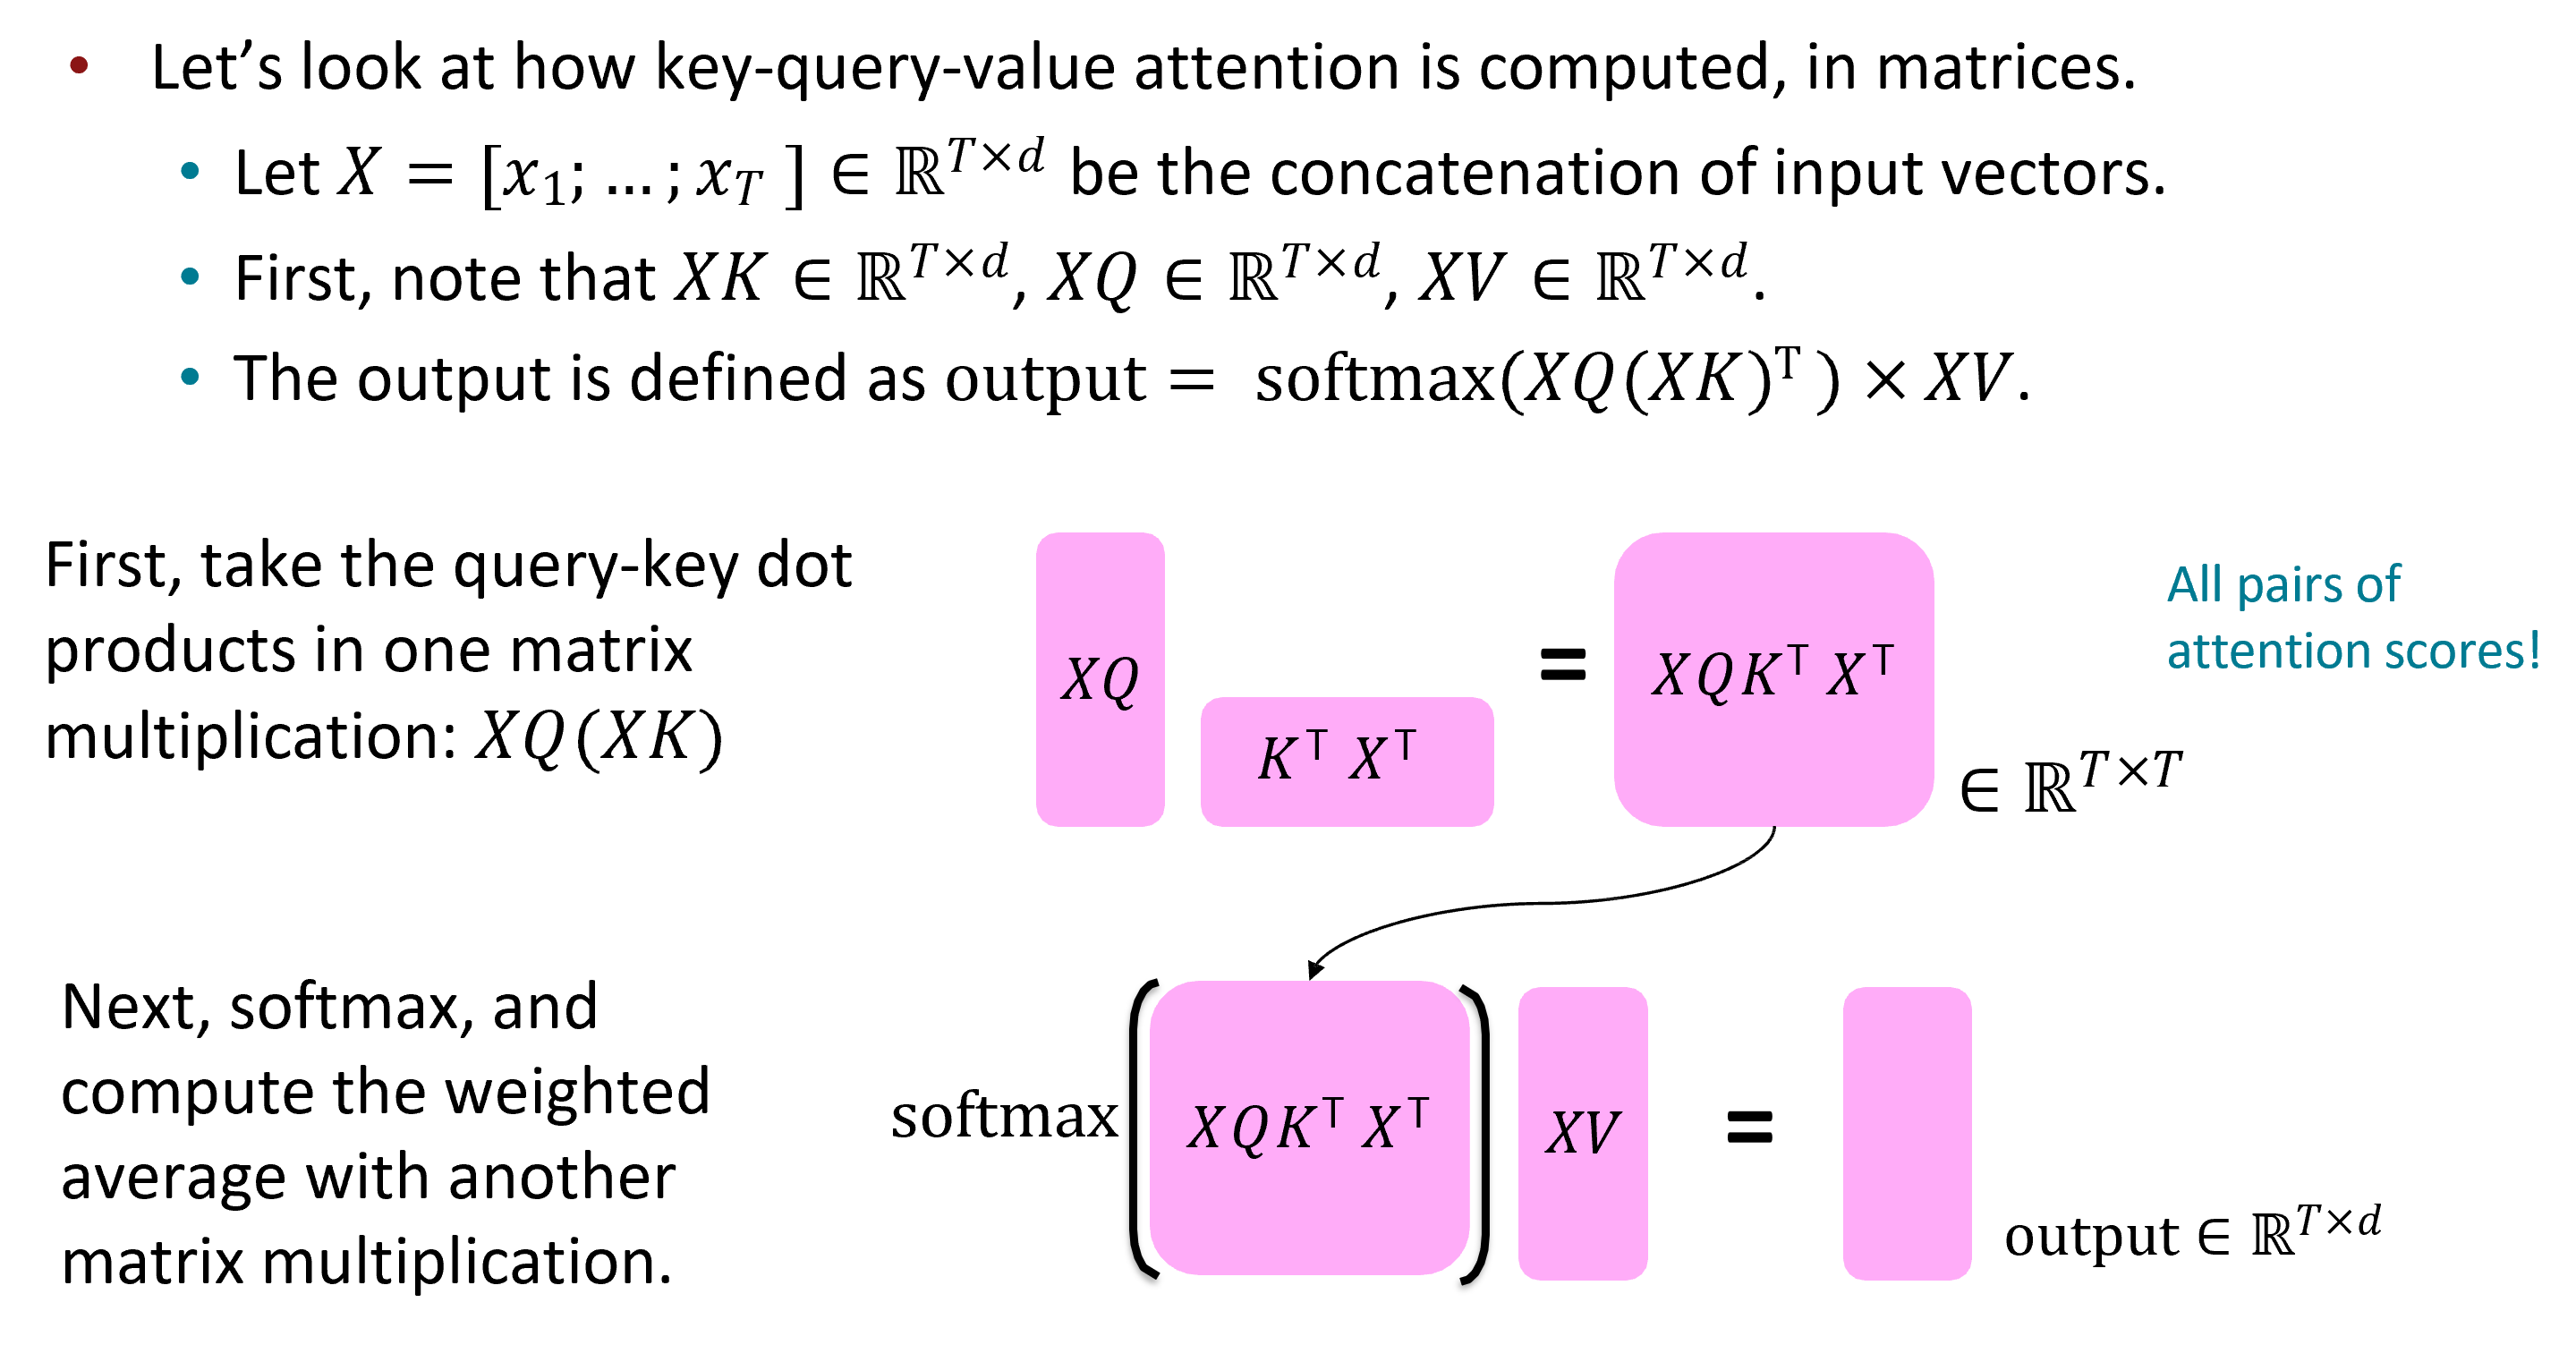
\includegraphics[width=\linewidth,keepaspectratio]{bert76}
			% \end{center}		
			
% % {\tiny (Ref: Language \& Machine Learning - John Hewitt)}

% \end{frame}

% %%%%%%%%%%%%%%%%%%%%%%%%%%%%%%%%%%%%%%%%%%%%%%%%%%%%%%%%%%%
% \begin{frame}[fragile]\frametitle{The Transformer Encoder: Multi-headed attention}

			
			% \begin{center}
			% 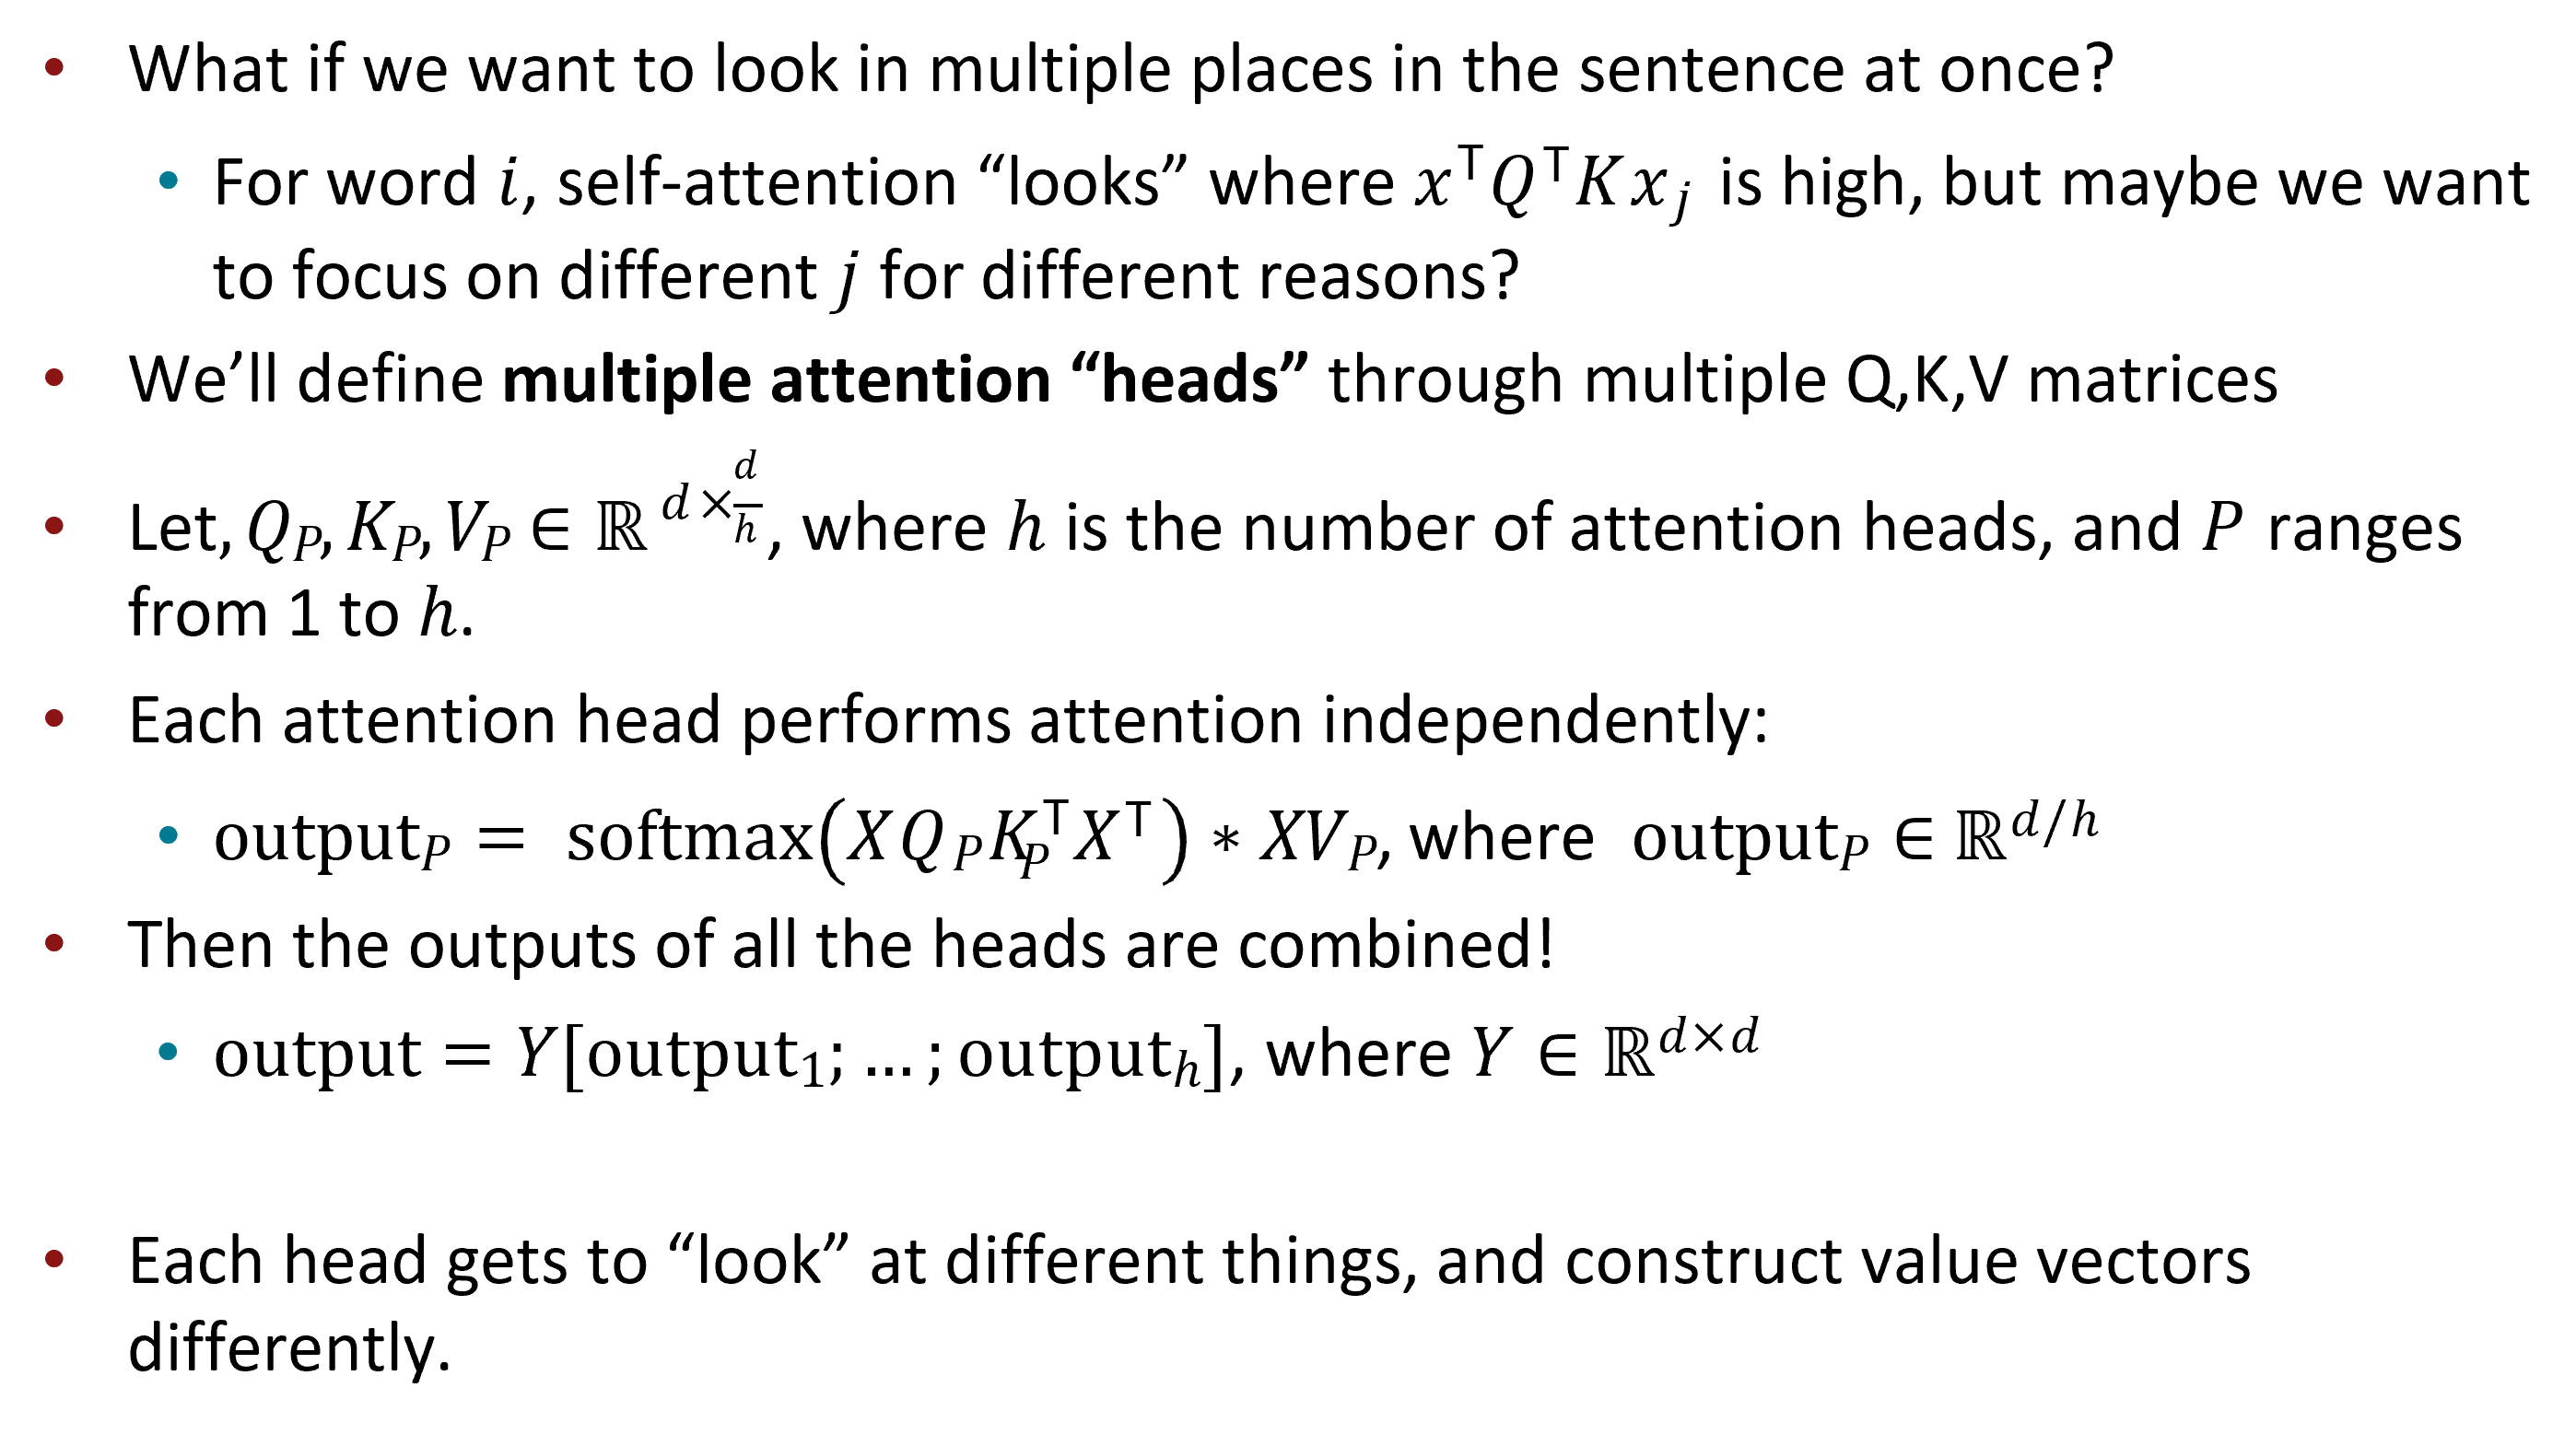
\includegraphics[width=\linewidth,keepaspectratio]{bert77}
			% \end{center}		
			
% % {\tiny (Ref: Language \& Machine Learning - John Hewitt)}

% \end{frame}

% %%%%%%%%%%%%%%%%%%%%%%%%%%%%%%%%%%%%%%%%%%%%%%%%%%%%%%%%%%%
% \begin{frame}[fragile]\frametitle{The Transformer Encoder: Multi-headed attention}

			
			% \begin{center}
			% 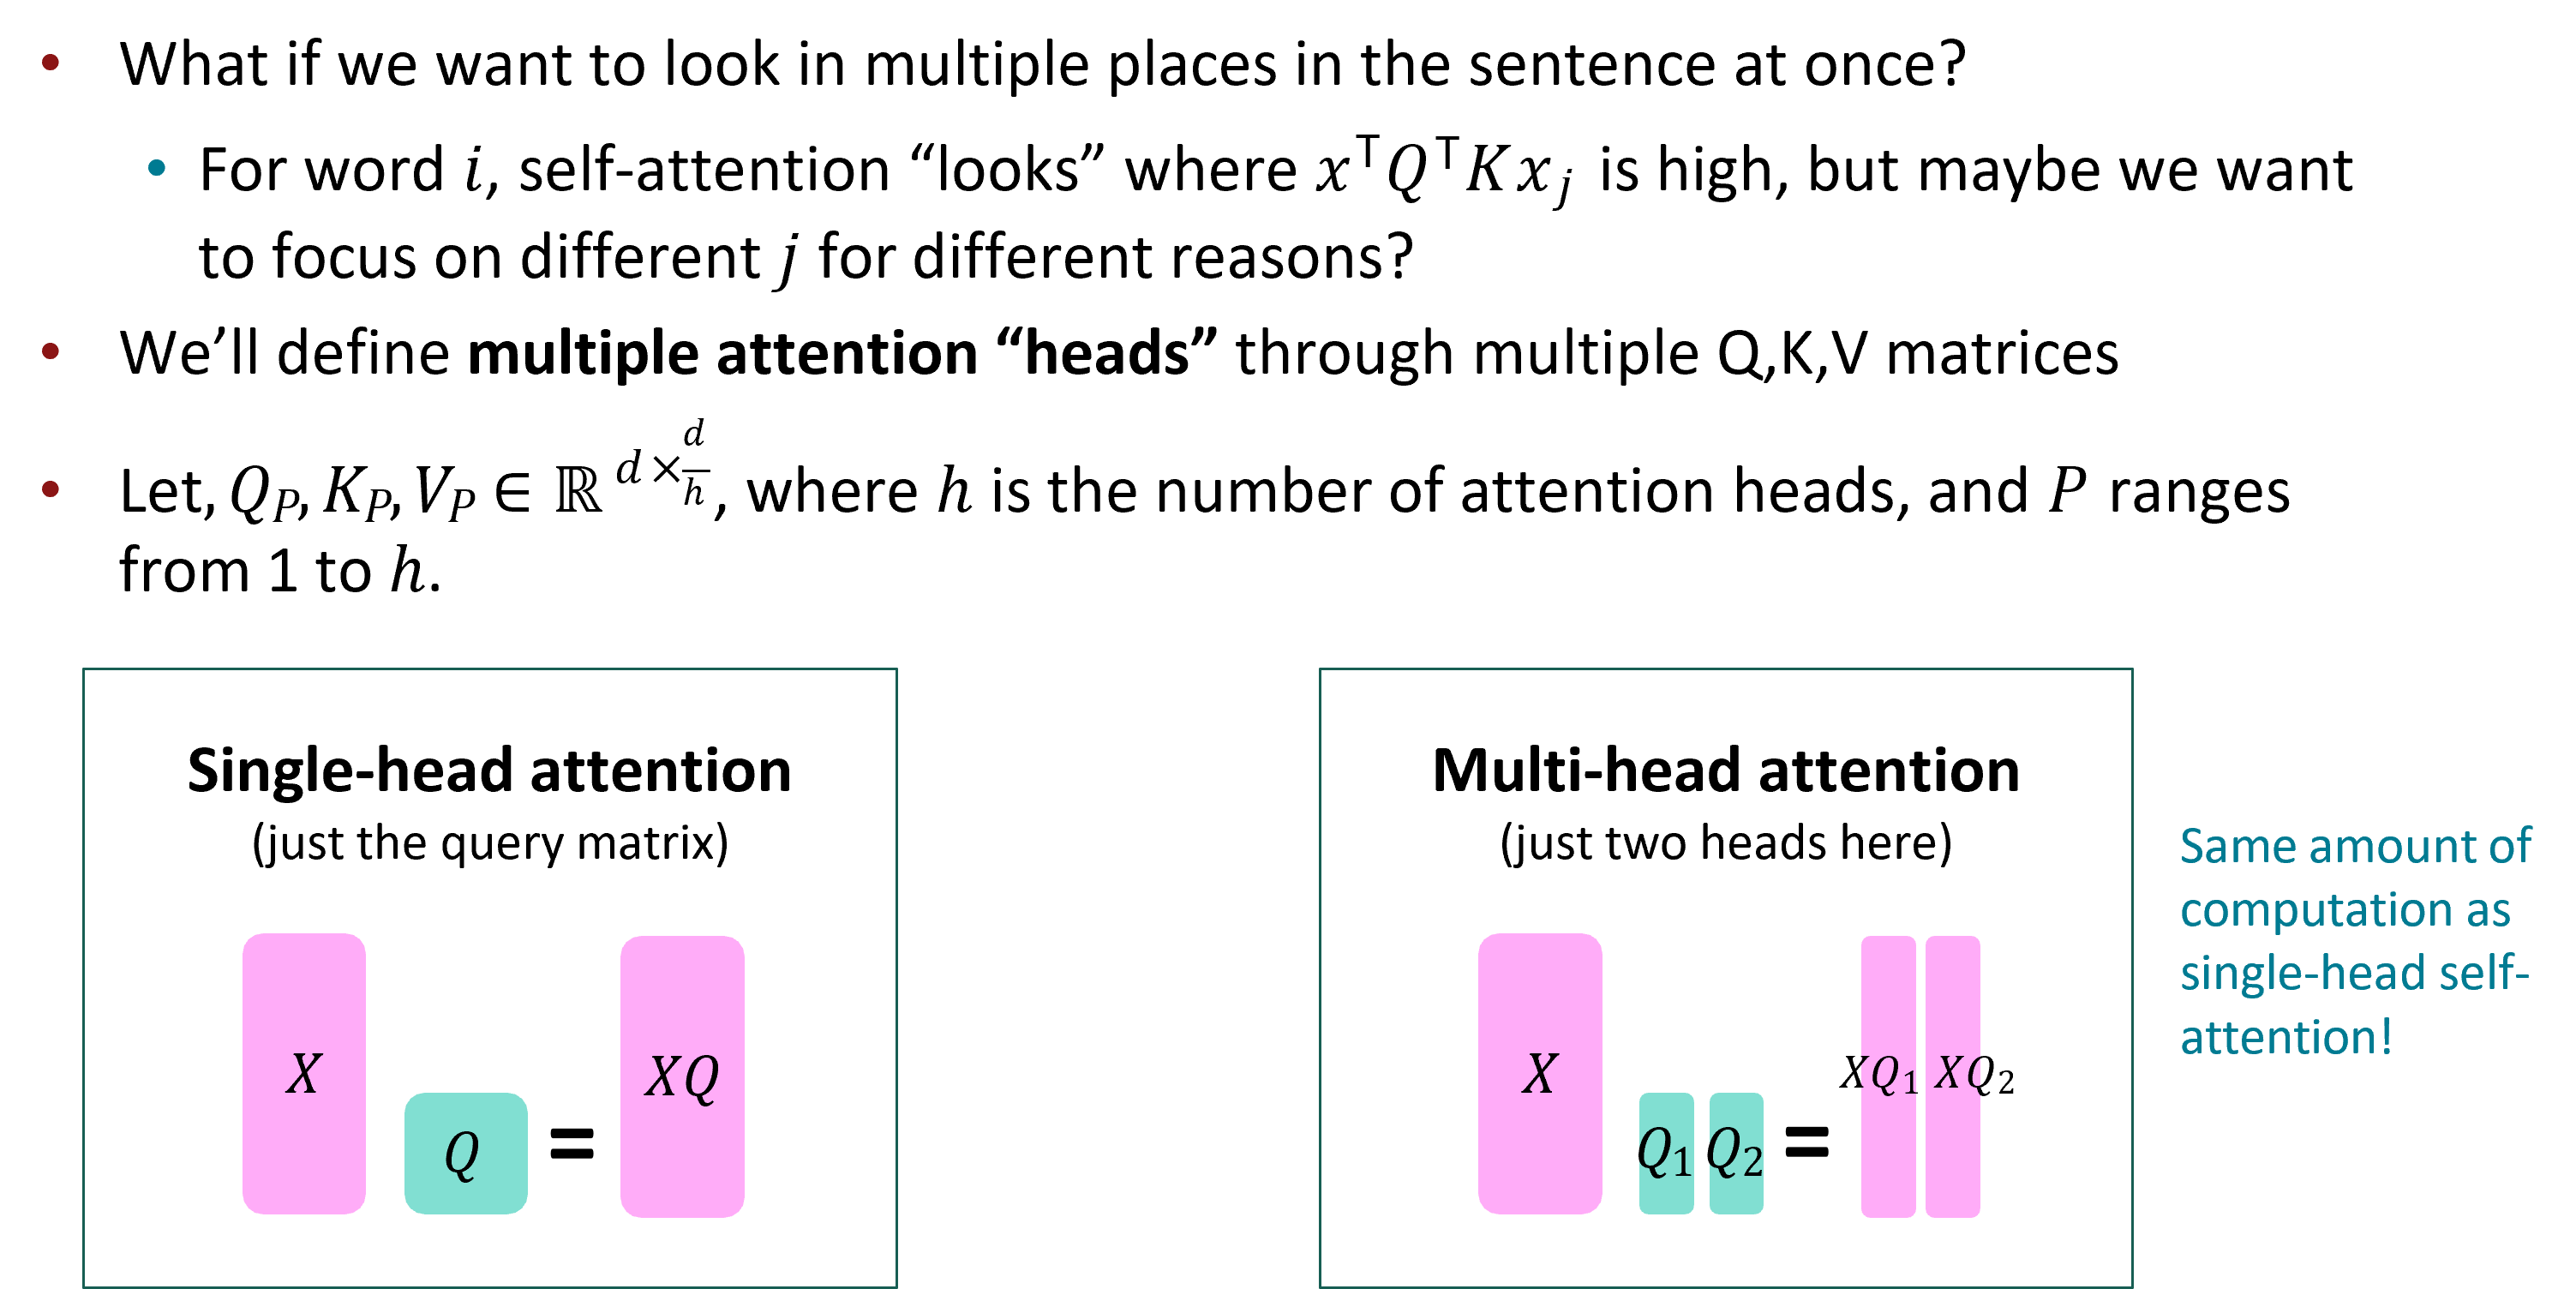
\includegraphics[width=\linewidth,keepaspectratio]{bert78}
			% \end{center}		
			
% % {\tiny (Ref: Language \& Machine Learning - John Hewitt)}

% \end{frame}

% %%%%%%%%%%%%%%%%%%%%%%%%%%%%%%%%%%%%%%%%%%%%%%%%%%%%%%%%%%%
% \begin{frame}[fragile]\frametitle{Attention visualization in layer 5}

			
			% \begin{center}
			% 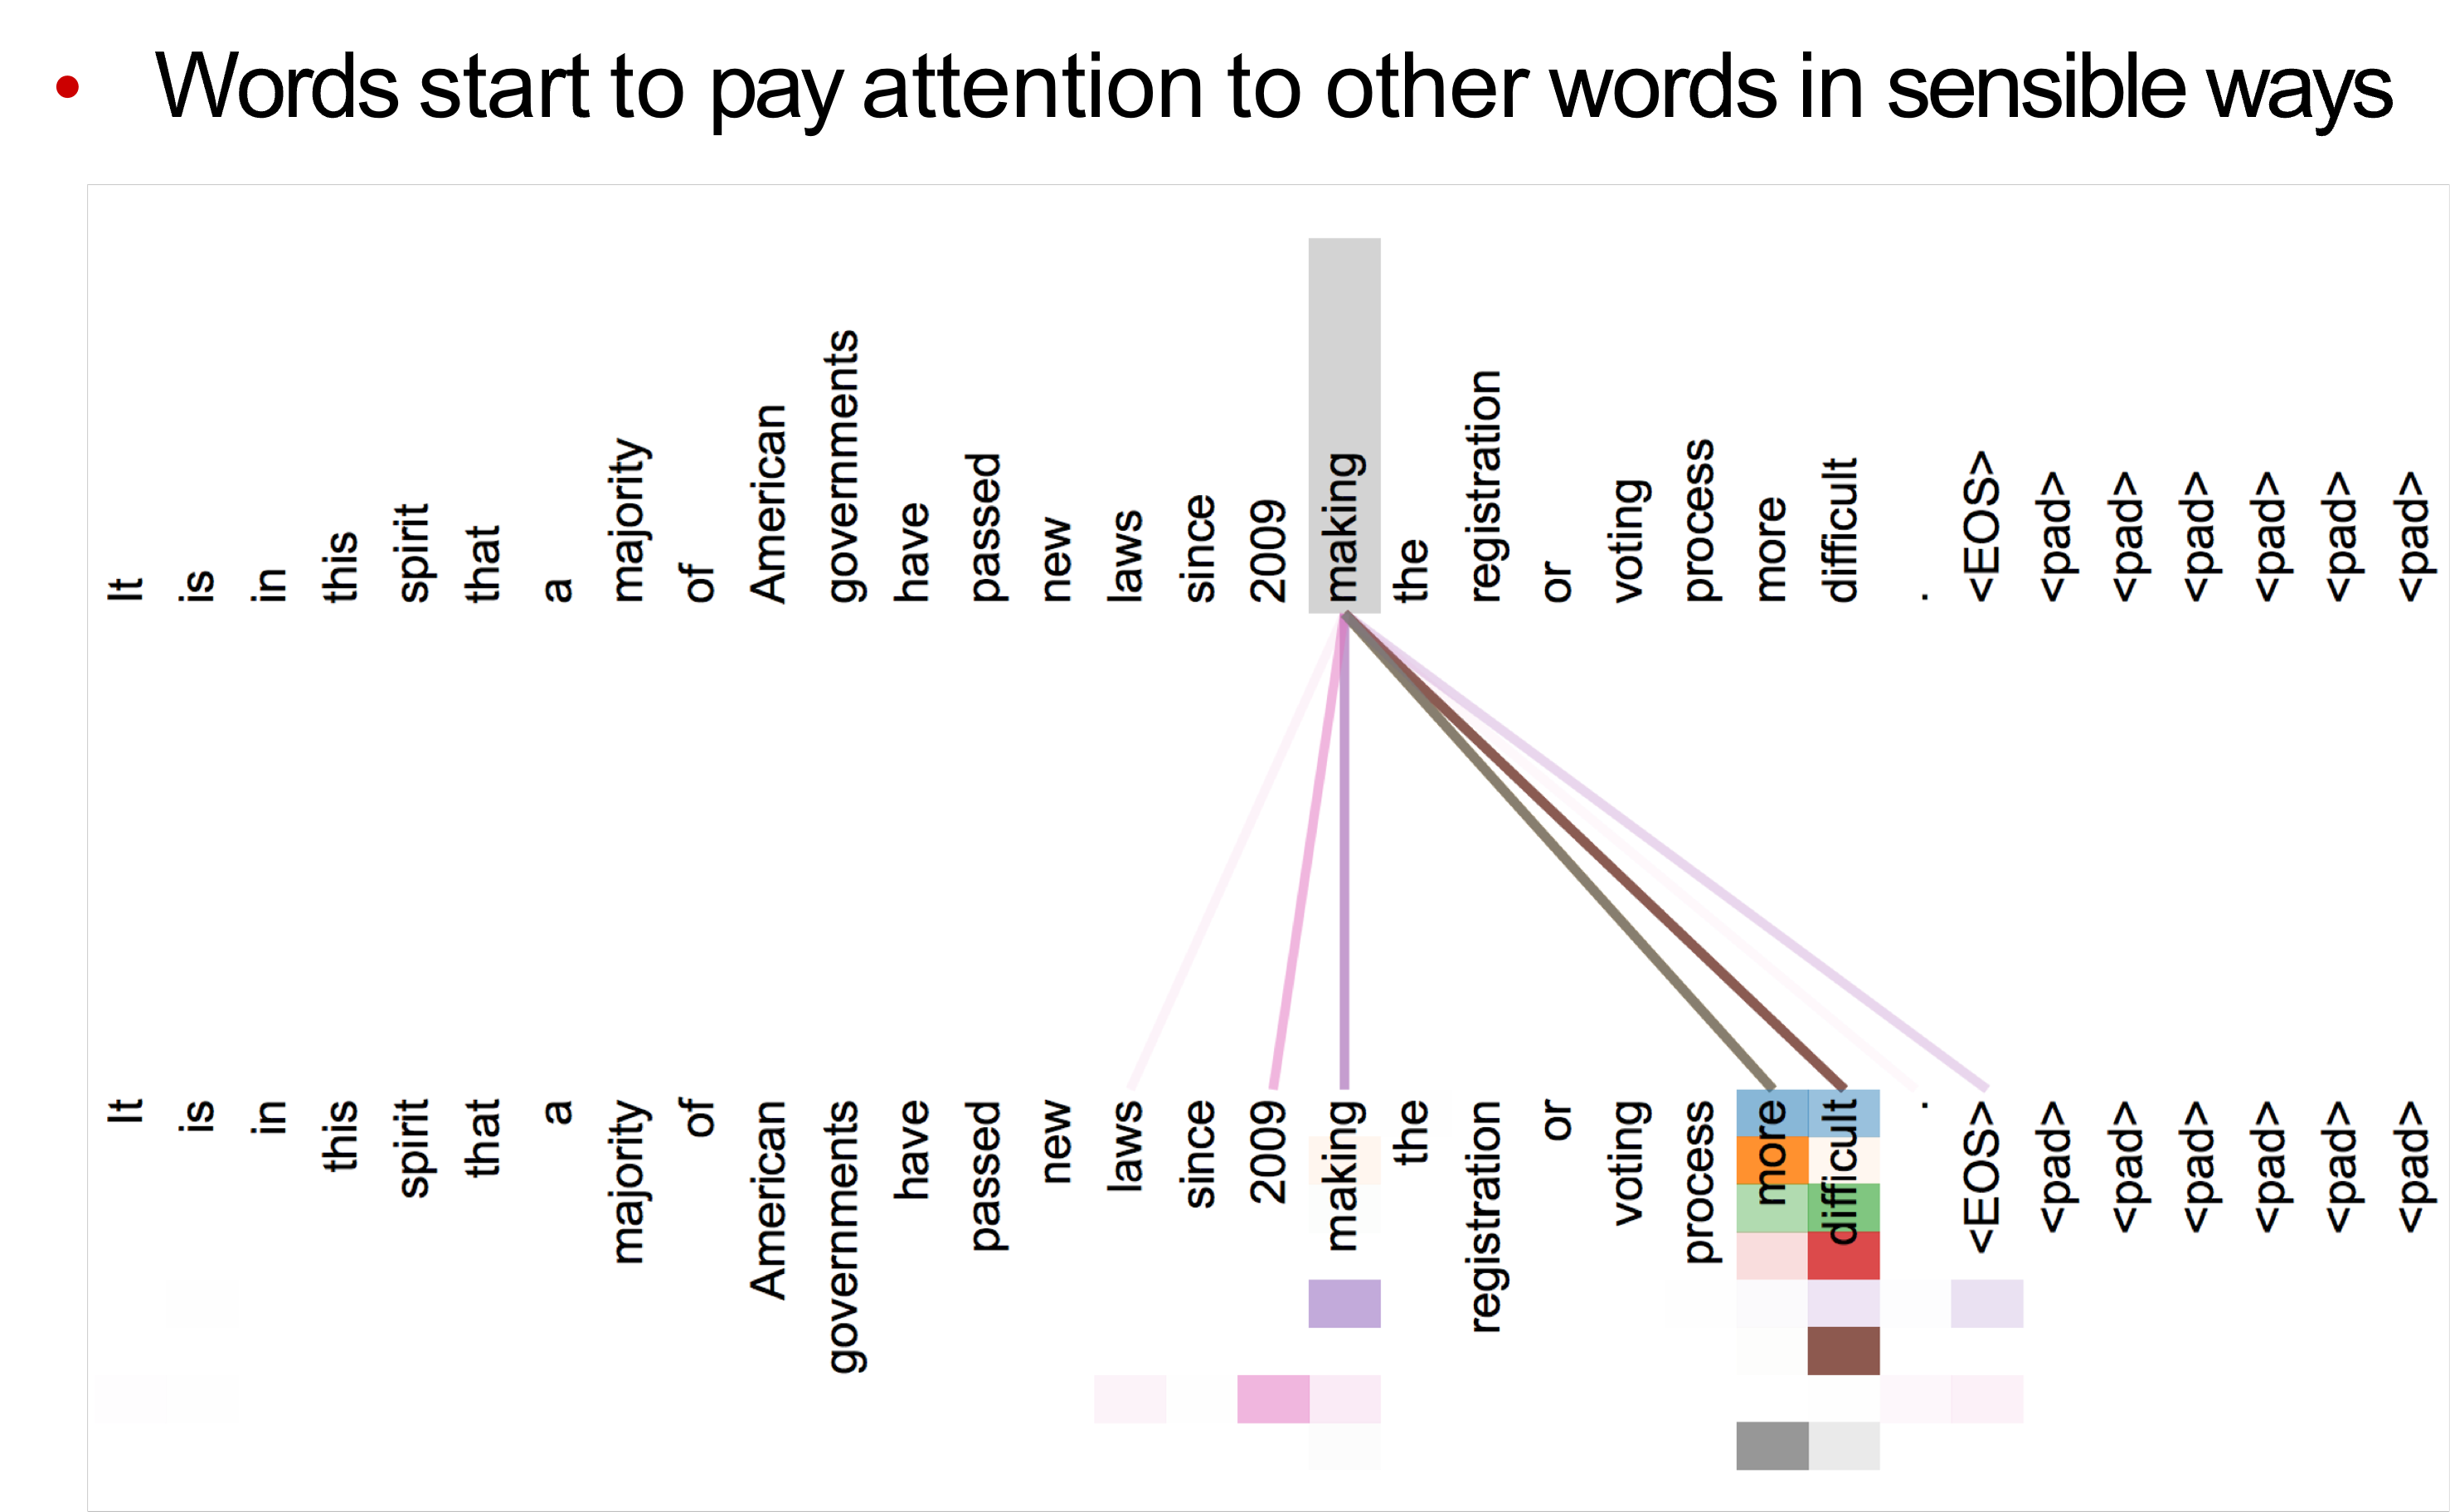
\includegraphics[width=0.8\linewidth,keepaspectratio]{bert79}
			% \end{center}		
			
			% % {\tiny (Ref: CS224n: Natural Language Processing with Deep Learning - Christopher Manning)}

% \end{frame}

% %%%%%%%%%%%%%%%%%%%%%%%%%%%%%%%%%%%%%%%%%%%%%%%%%%%%%%%%%%%
% \begin{frame}[fragile]\frametitle{Attention visualization: Implicit anaphora resolution}

			
			% \begin{center}
			% 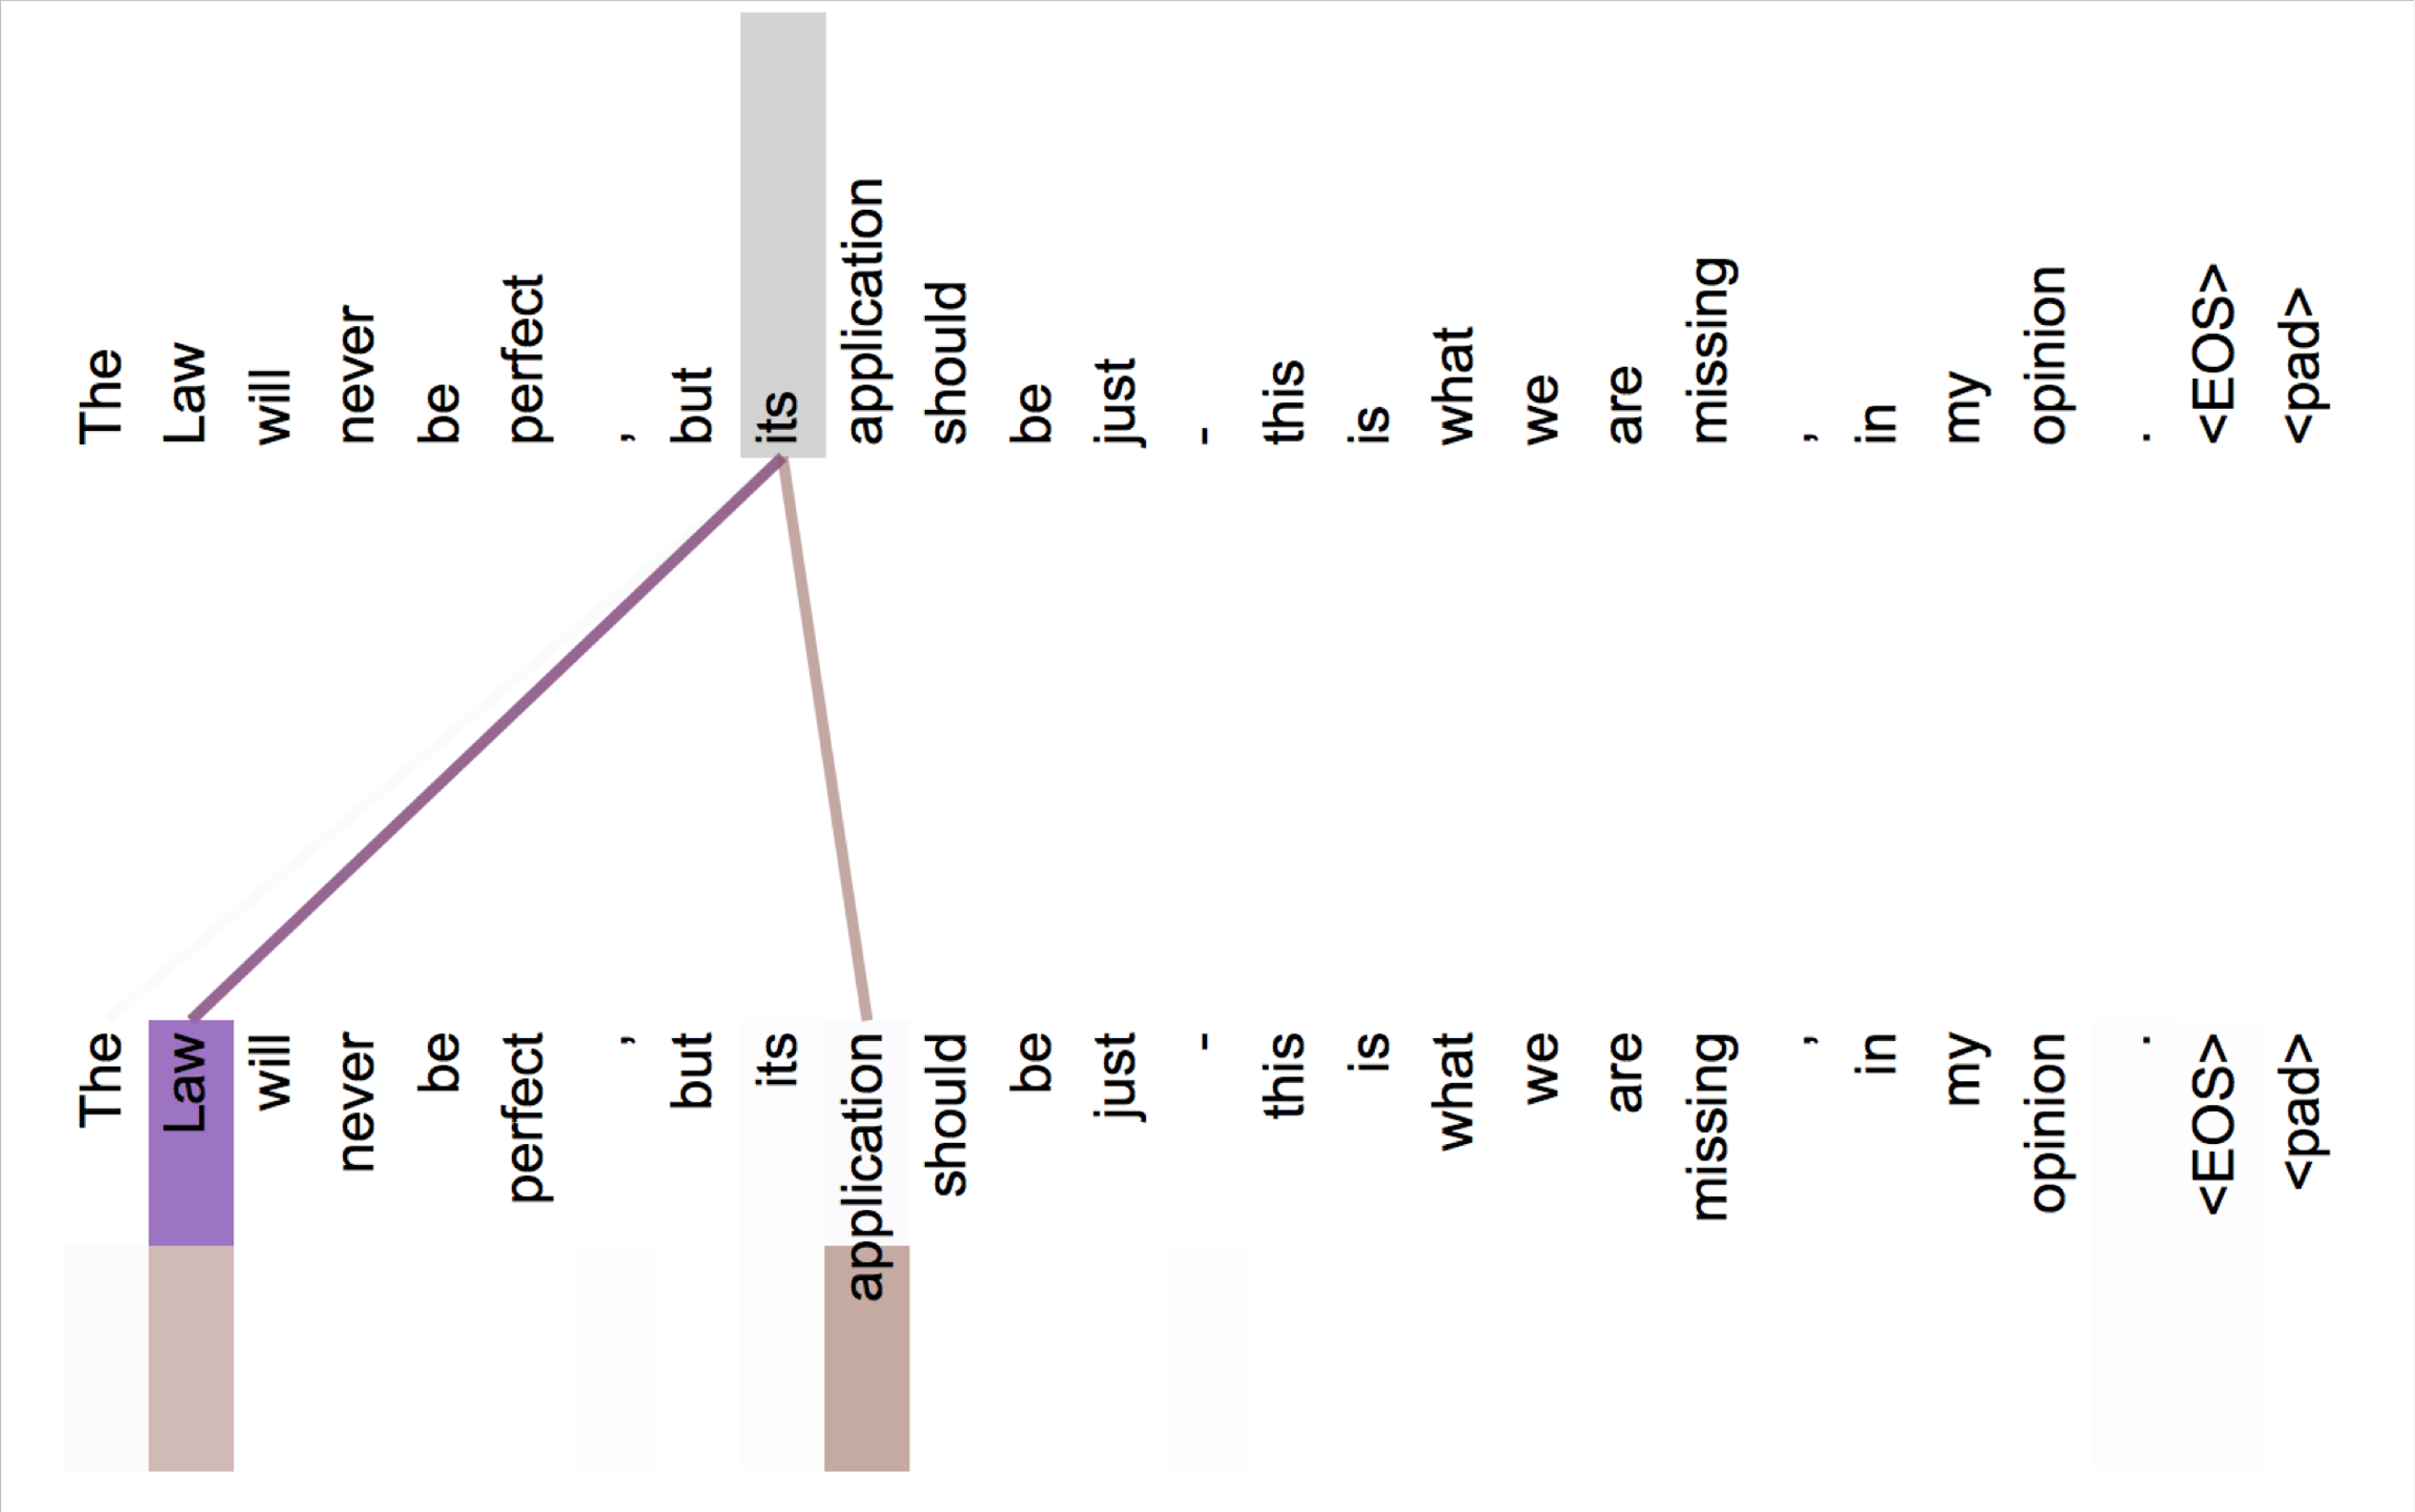
\includegraphics[width=0.6\linewidth,keepaspectratio]{bert80}
			% \end{center}		
			
			% In 5th layer. Isolated attentions from just the word ‘its’ for attention heads 5 and 6.  Note that the attentions are very sharp for this word.

			
			% % {\tiny (Ref: CS224n: Natural Language Processing with Deep Learning - Christopher Manning)}

% \end{frame}

% %%%%%%%%%%%%%%%%%%%%%%%%%%%%%%%%%%%%%%%%%%%%%%%%%%%%%%%%%%%
% \begin{frame}[fragile]\frametitle{Parallel attention heads}

			
			% \begin{center}
			% 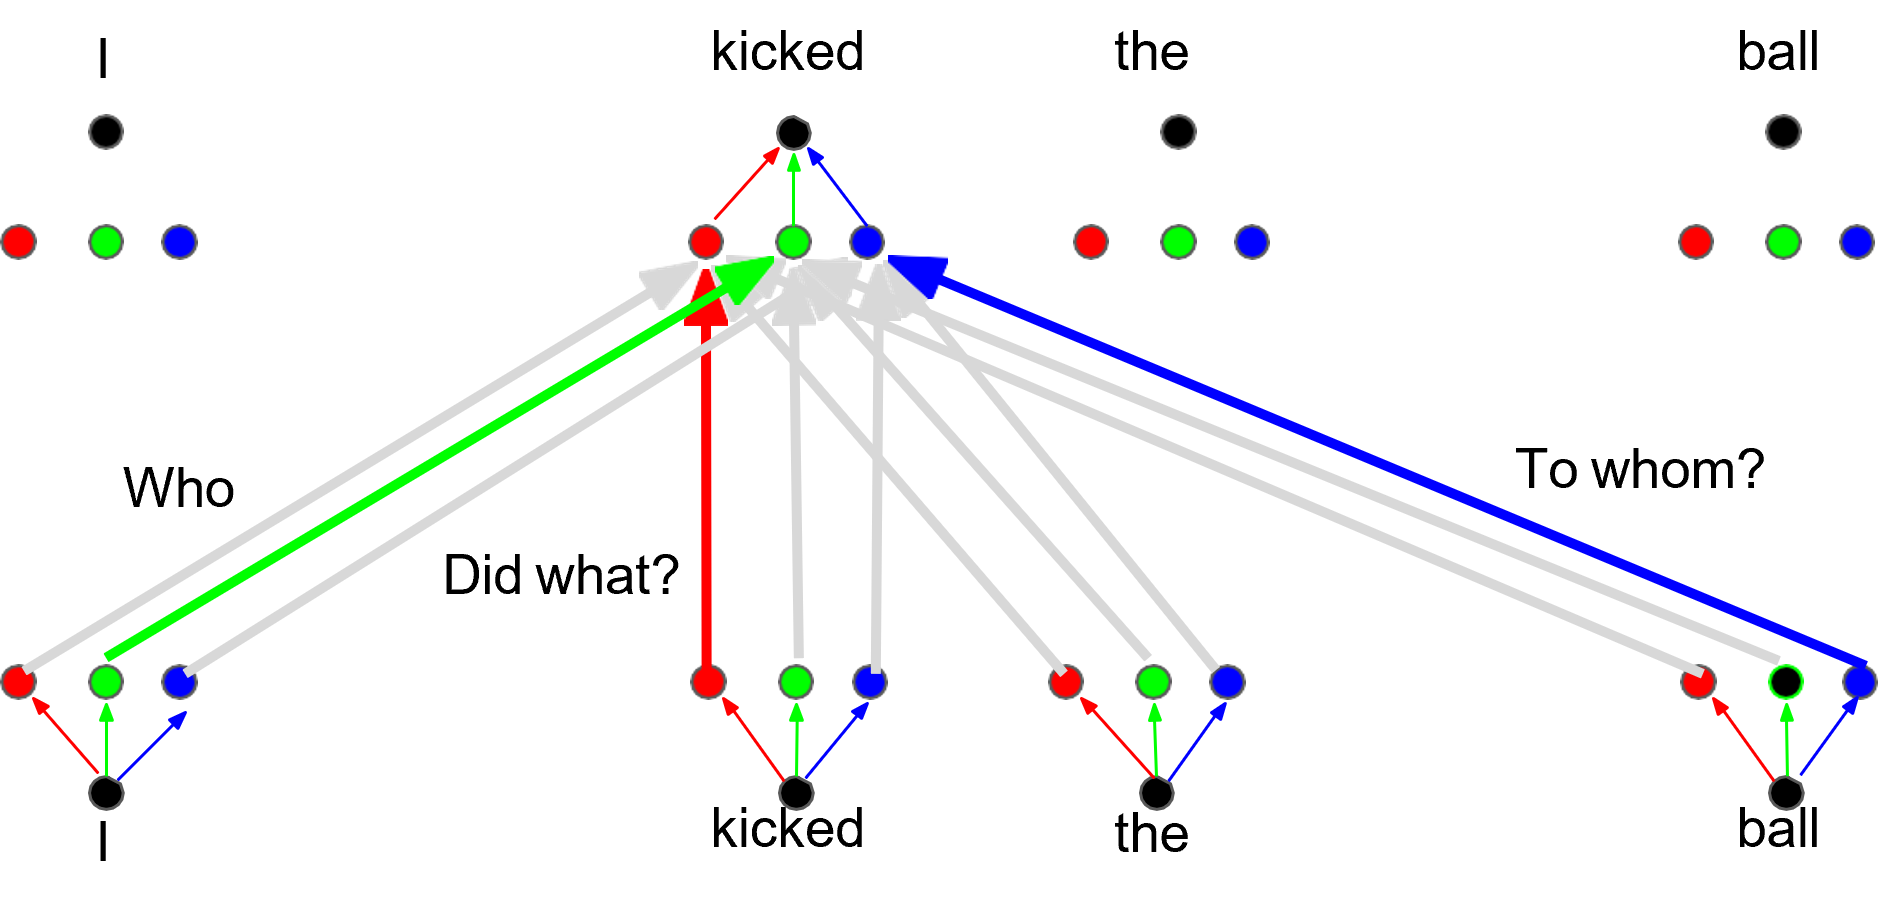
\includegraphics[width=0.6\linewidth,keepaspectratio]{bert81}
			% \end{center}		
			
		
			% % {\tiny (Ref: Ashish Vaswani)}

% \end{frame}

% %%%%%%%%%%%%%%%%%%%%%%%%%%%%%%%%%%%%%%%%%%%%%%%%%%%%%%%%%%%
% \begin{frame}[fragile]\frametitle{Residual connections}

			% The Transformer Encoder: Residual connections [He et al., 2016]
			
			% \begin{center}
			% 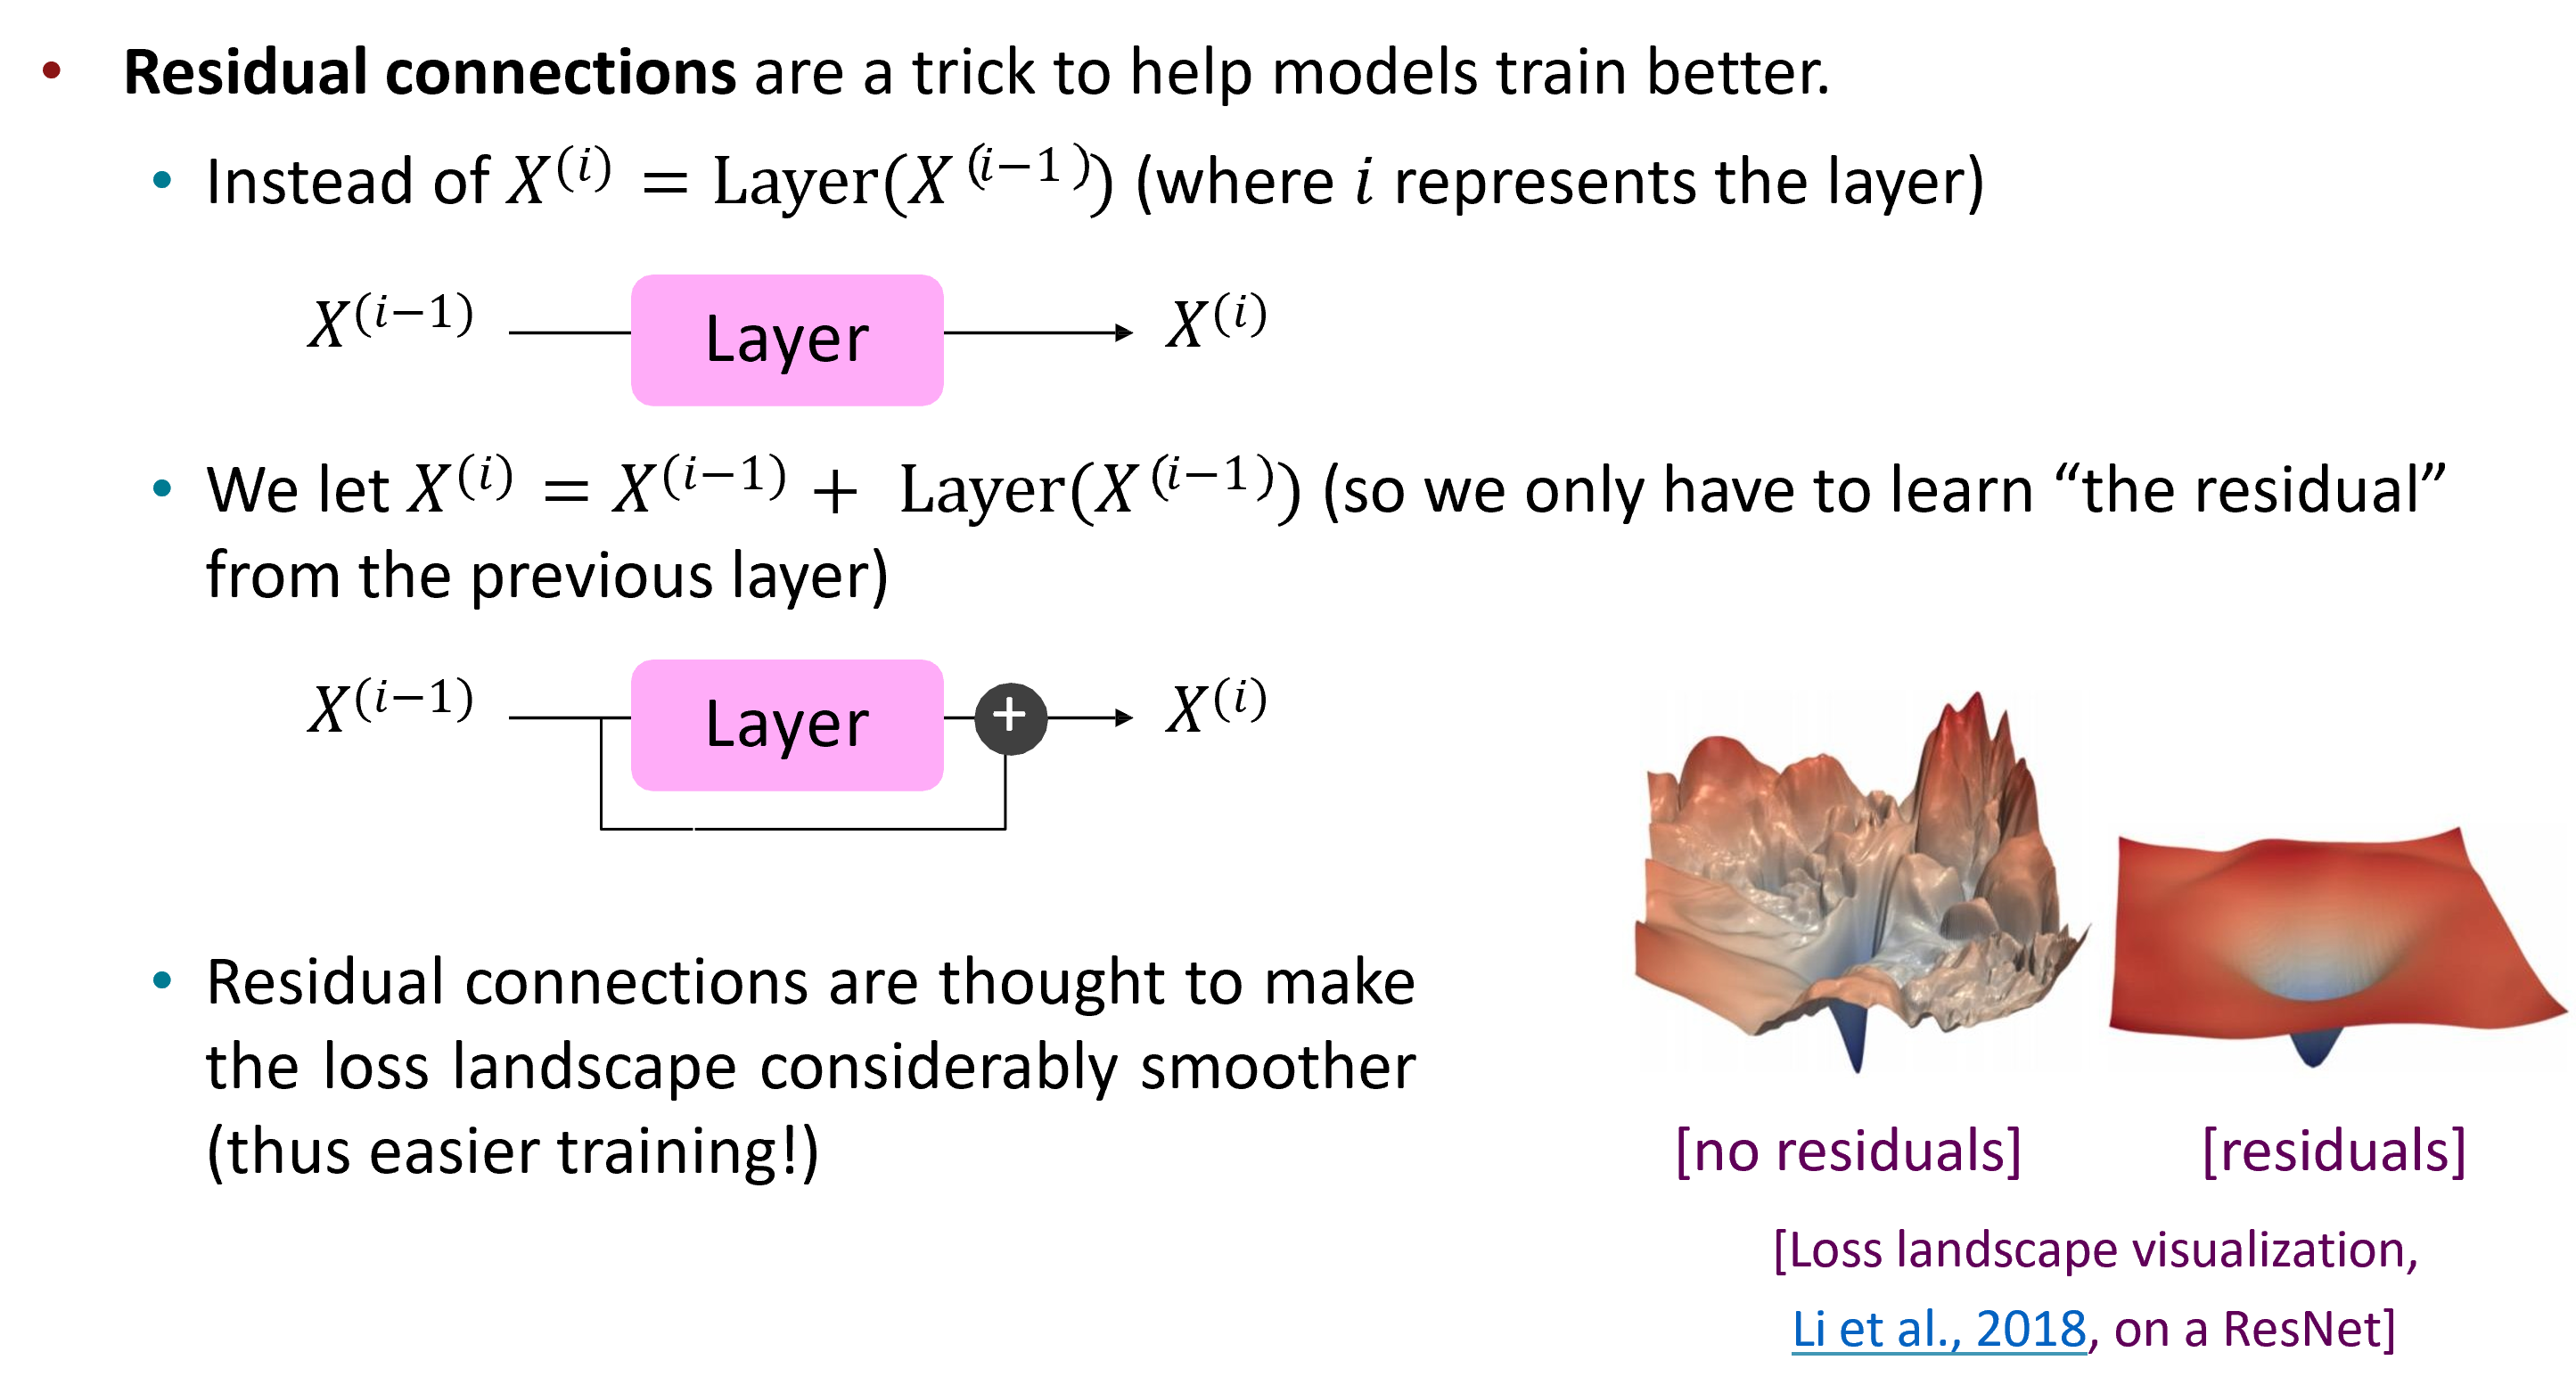
\includegraphics[width=\linewidth,keepaspectratio]{bert82}
			% \end{center}		
			
		
			% % {\tiny (Ref: John Hewitt)}

% \end{frame}

% %%%%%%%%%%%%%%%%%%%%%%%%%%%%%%%%%%%%%%%%%%%%%%%%%%%%%%%%%%%
% \begin{frame}[fragile]\frametitle{Layer normalization}
% The Transformer Encoder: Layer normalization [Ba et al., 2016]
			
			% \begin{center}
			% 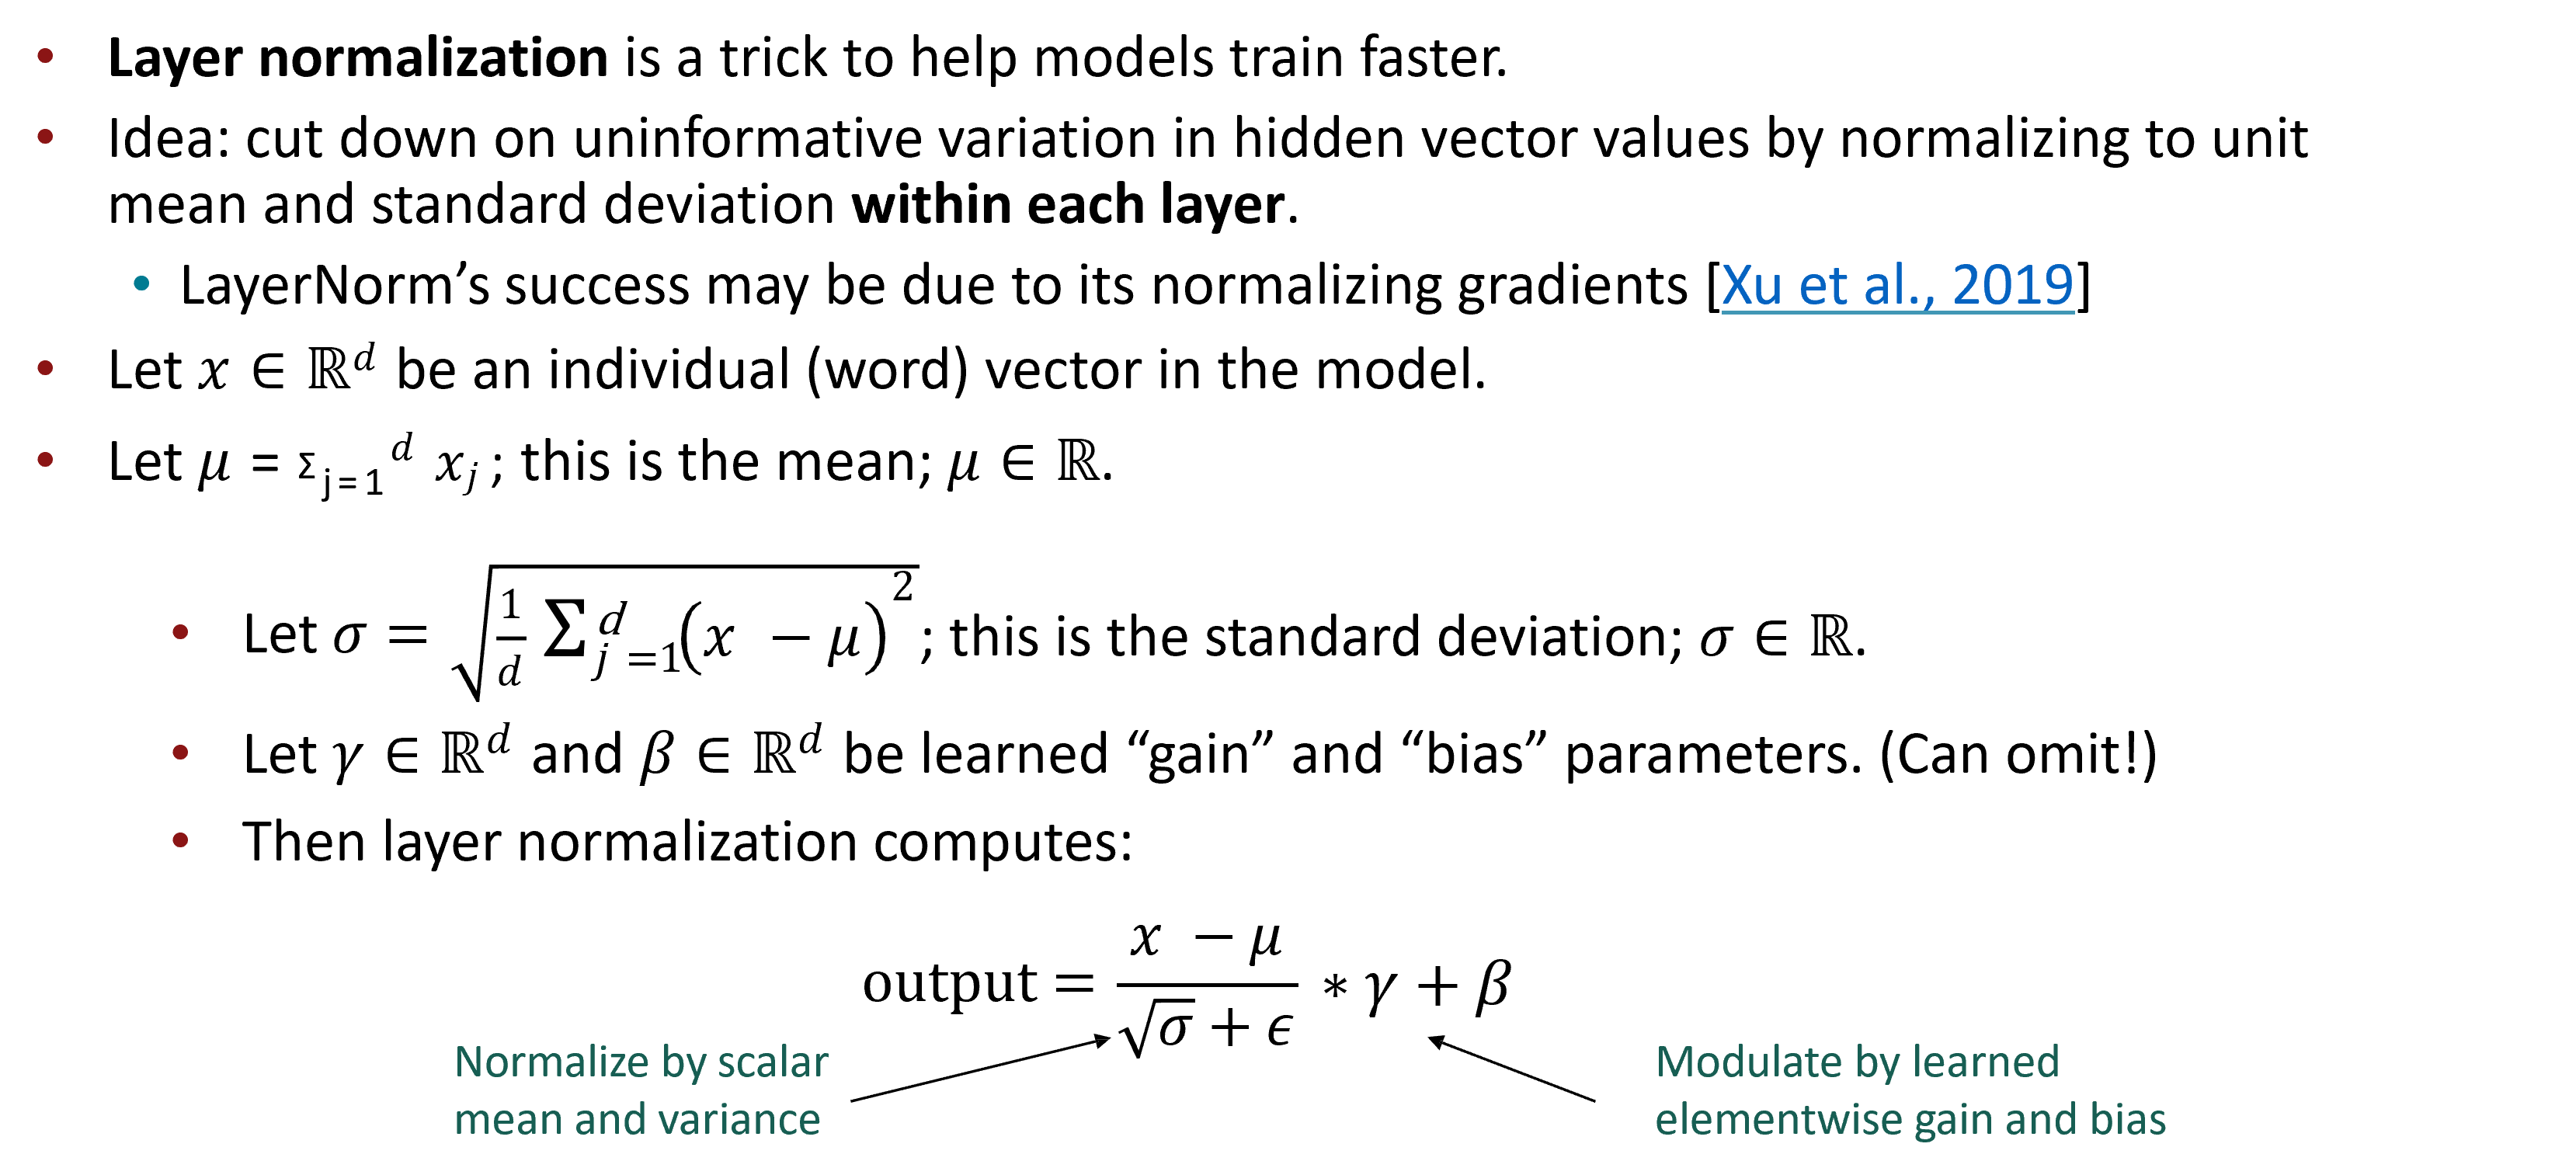
\includegraphics[width=\linewidth,keepaspectratio]{bert83}
			% \end{center}		
			
		
			% % {\tiny (Ref: John Hewitt)}

% \end{frame}

% %%%%%%%%%%%%%%%%%%%%%%%%%%%%%%%%%%%%%%%%%%%%%%%%%%%%%%%%%%%
% \begin{frame}[fragile]\frametitle{ Scaled Dot Product}

			% The Transformer Encoder: Scaled Dot Product [Vaswani et al., 2017]
			% \begin{center}
			% 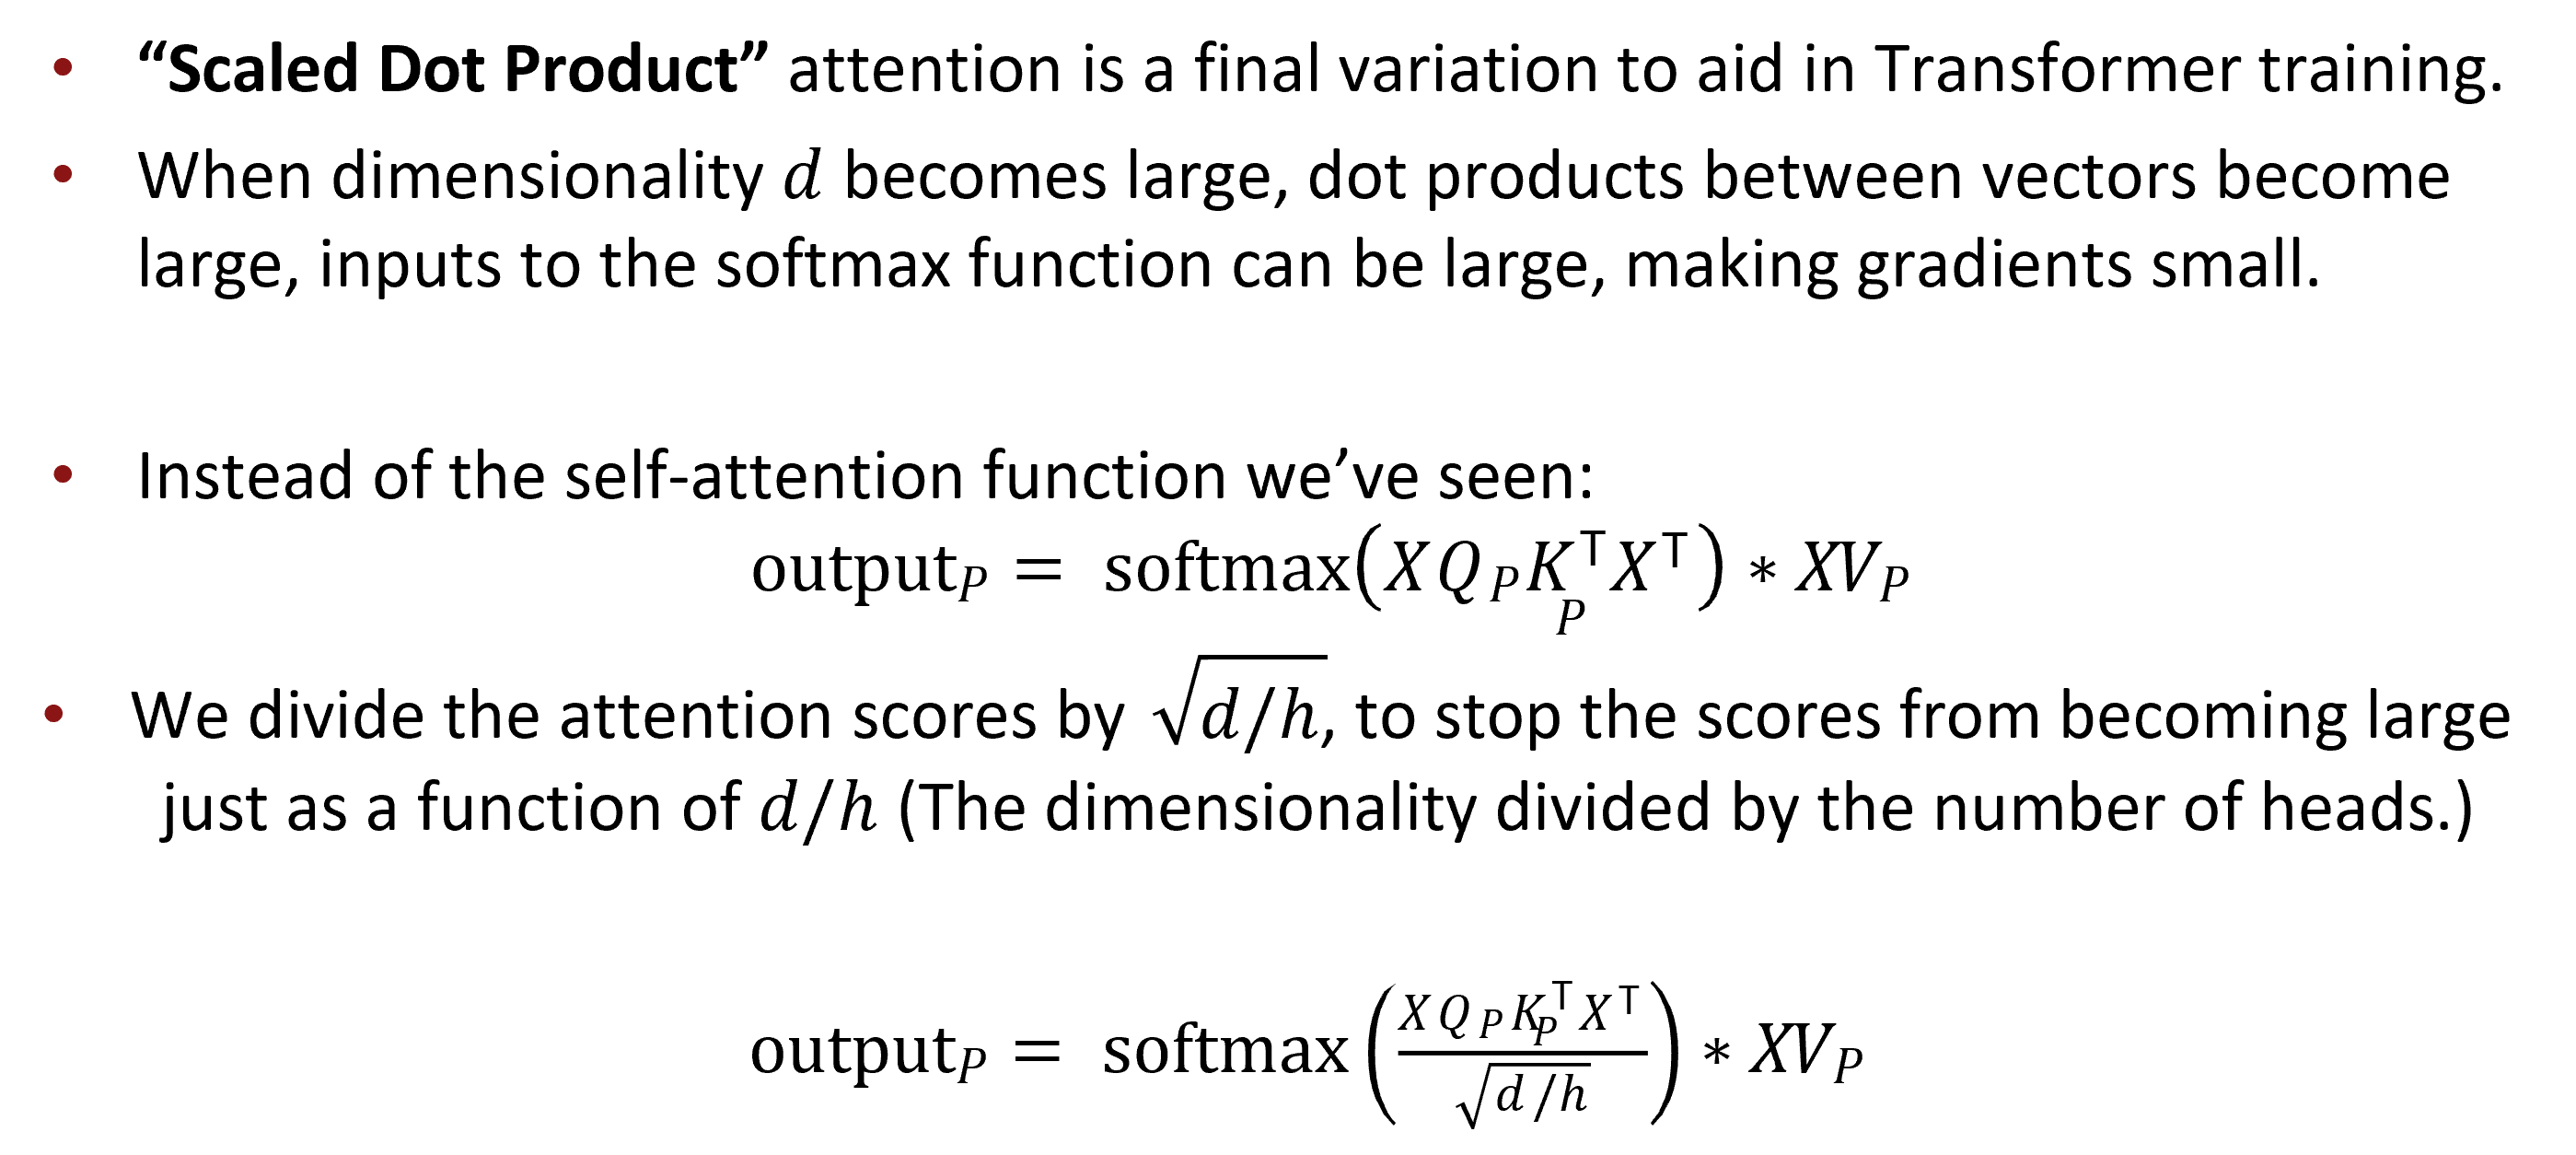
\includegraphics[width=\linewidth,keepaspectratio]{bert84}
			% \end{center}		
			
		
			% % {\tiny (Ref: John Hewitt)}

% \end{frame}

% %%%%%%%%%%%%%%%%%%%%%%%%%%%%%%%%%%%%%%%%%%%%%%%%%%%%%%%%%%%
% \begin{frame}[fragile]\frametitle{Scaled Dot Product}

% The Transformer Encoder: Scaled Dot Product [Vaswani et al., 2017]
			
			% \begin{center}
			% 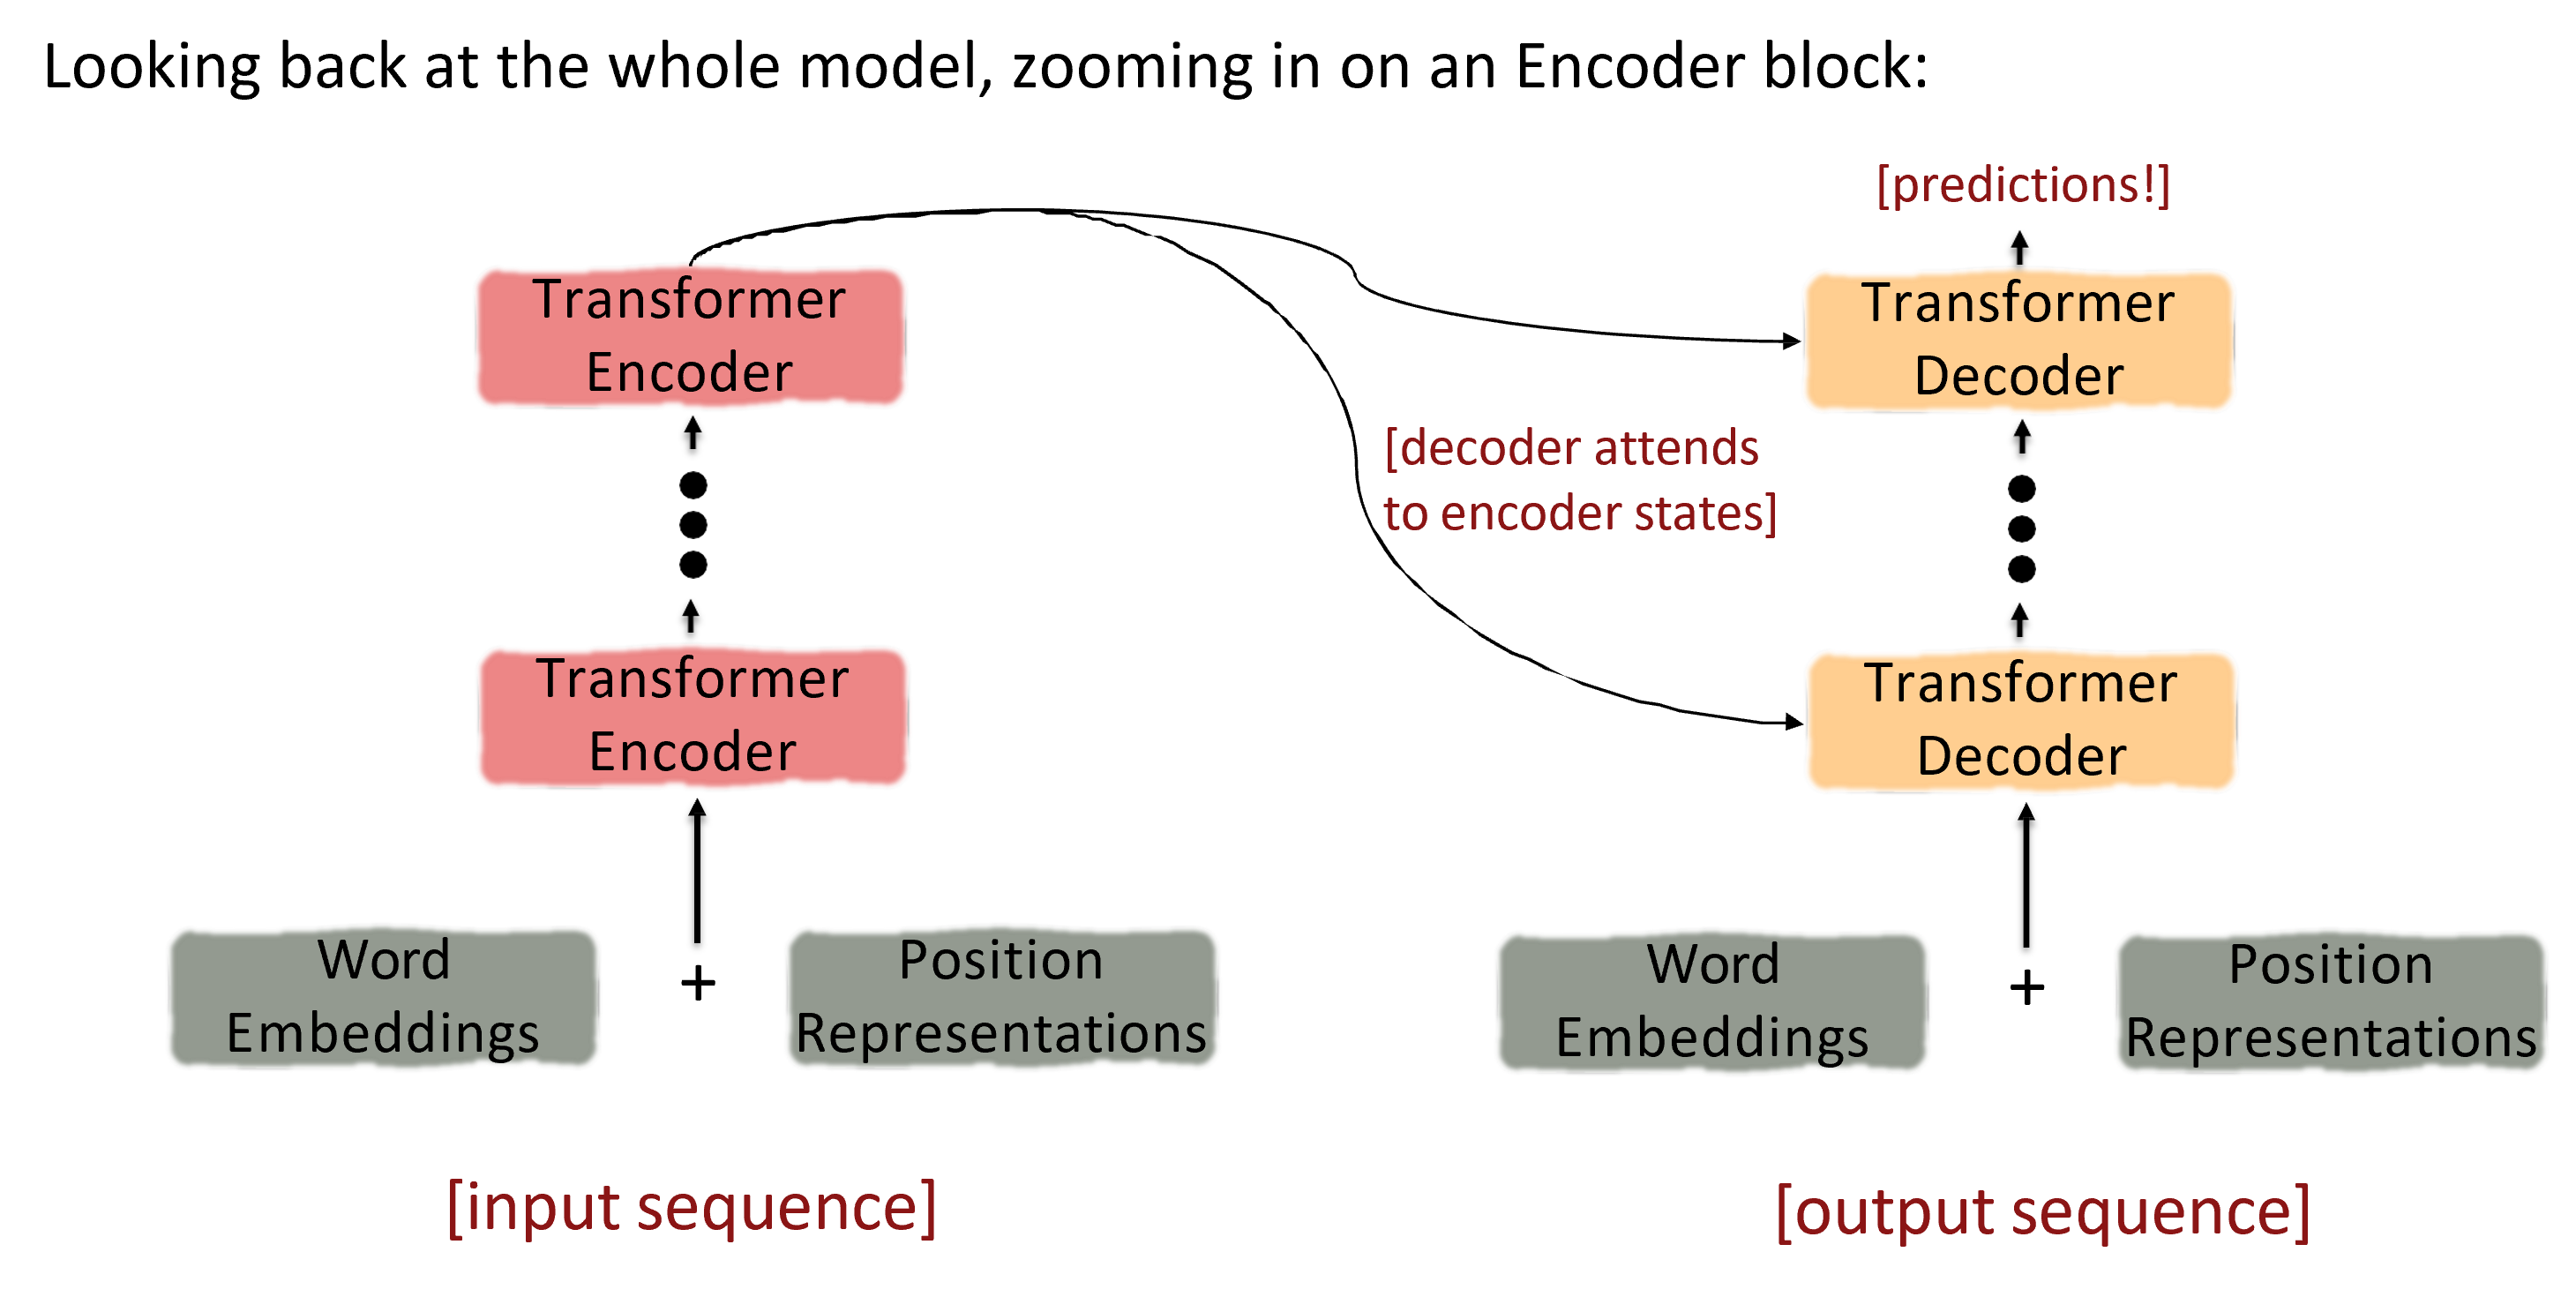
\includegraphics[width=\linewidth,keepaspectratio]{bert85}
			% \end{center}		
			
		
			% % {\tiny (Ref: John Hewitt)}

% \end{frame}

% %%%%%%%%%%%%%%%%%%%%%%%%%%%%%%%%%%%%%%%%%%%%%%%%%%%%%%%%%%%
% \begin{frame}[fragile]\frametitle{Scaled Dot Product}

			% The Transformer Encoder: Scaled Dot Product [Vaswani et al., 2017]
			
			% \begin{center}
			% 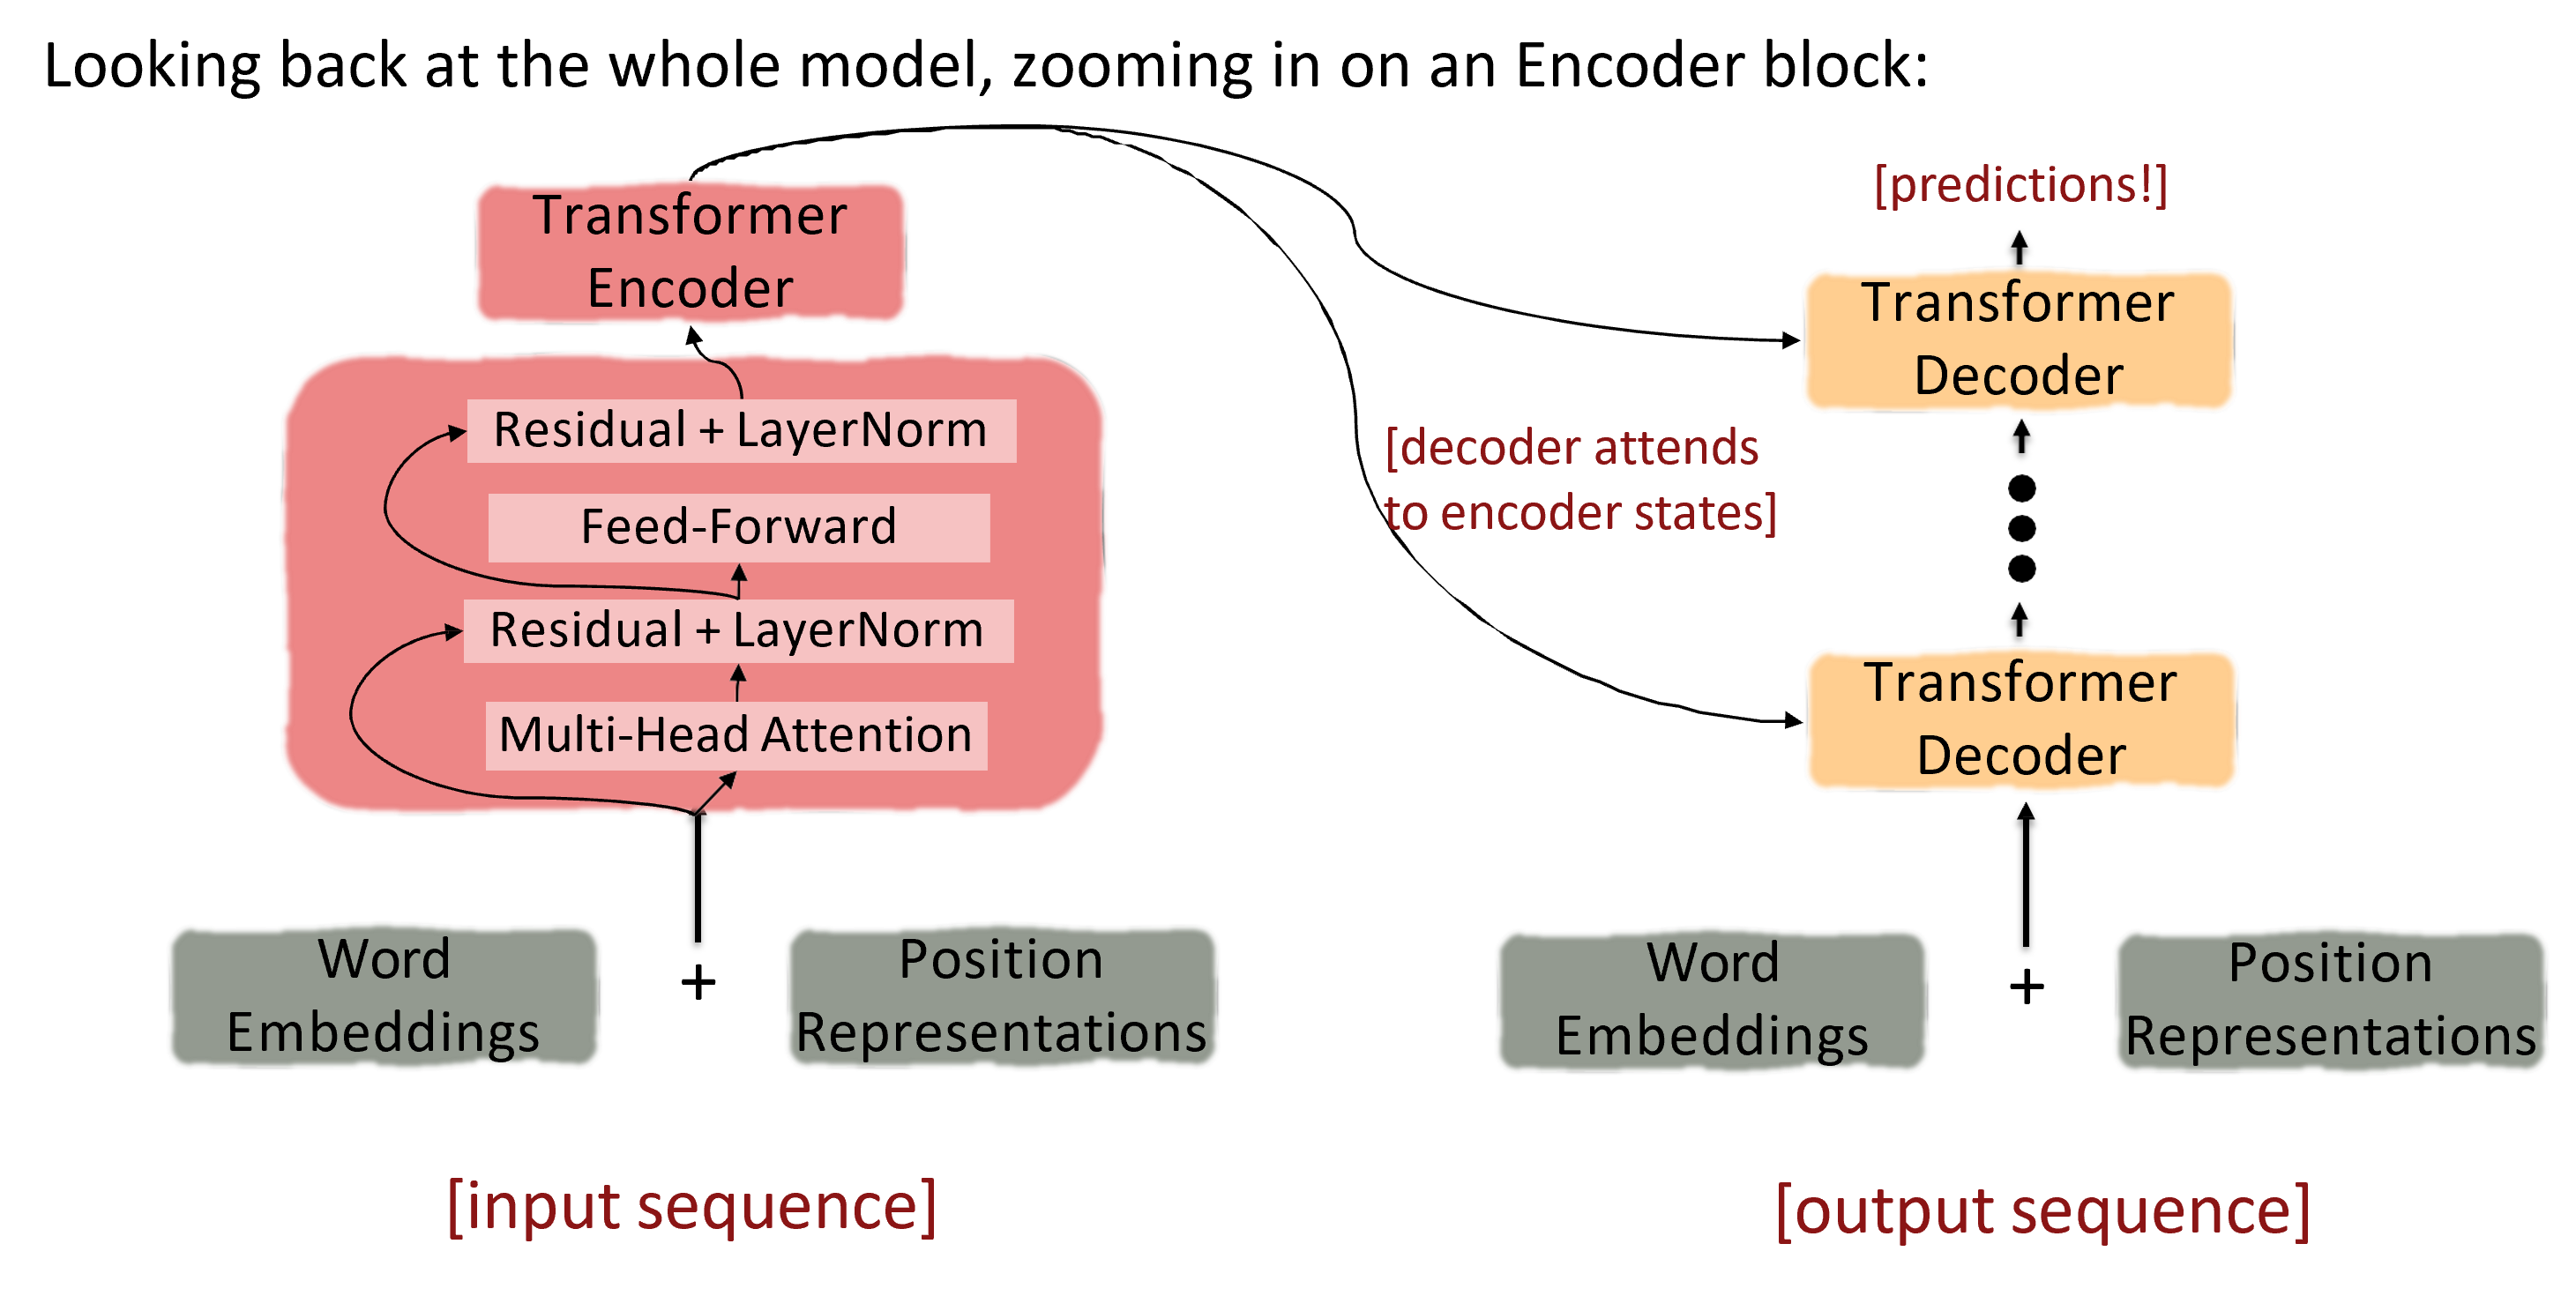
\includegraphics[width=\linewidth,keepaspectratio]{bert86}
			% \end{center}		
			
		
			% % {\tiny (Ref: John Hewitt)}

% \end{frame}

% %%%%%%%%%%%%%%%%%%%%%%%%%%%%%%%%%%%%%%%%%%%%%%%%%%%%%%%%%%%
% \begin{frame}[fragile]\frametitle{Scaled Dot Product}

						% The Transformer Encoder: Scaled Dot Product [Vaswani et al., 2017]

			% \begin{center}
			% 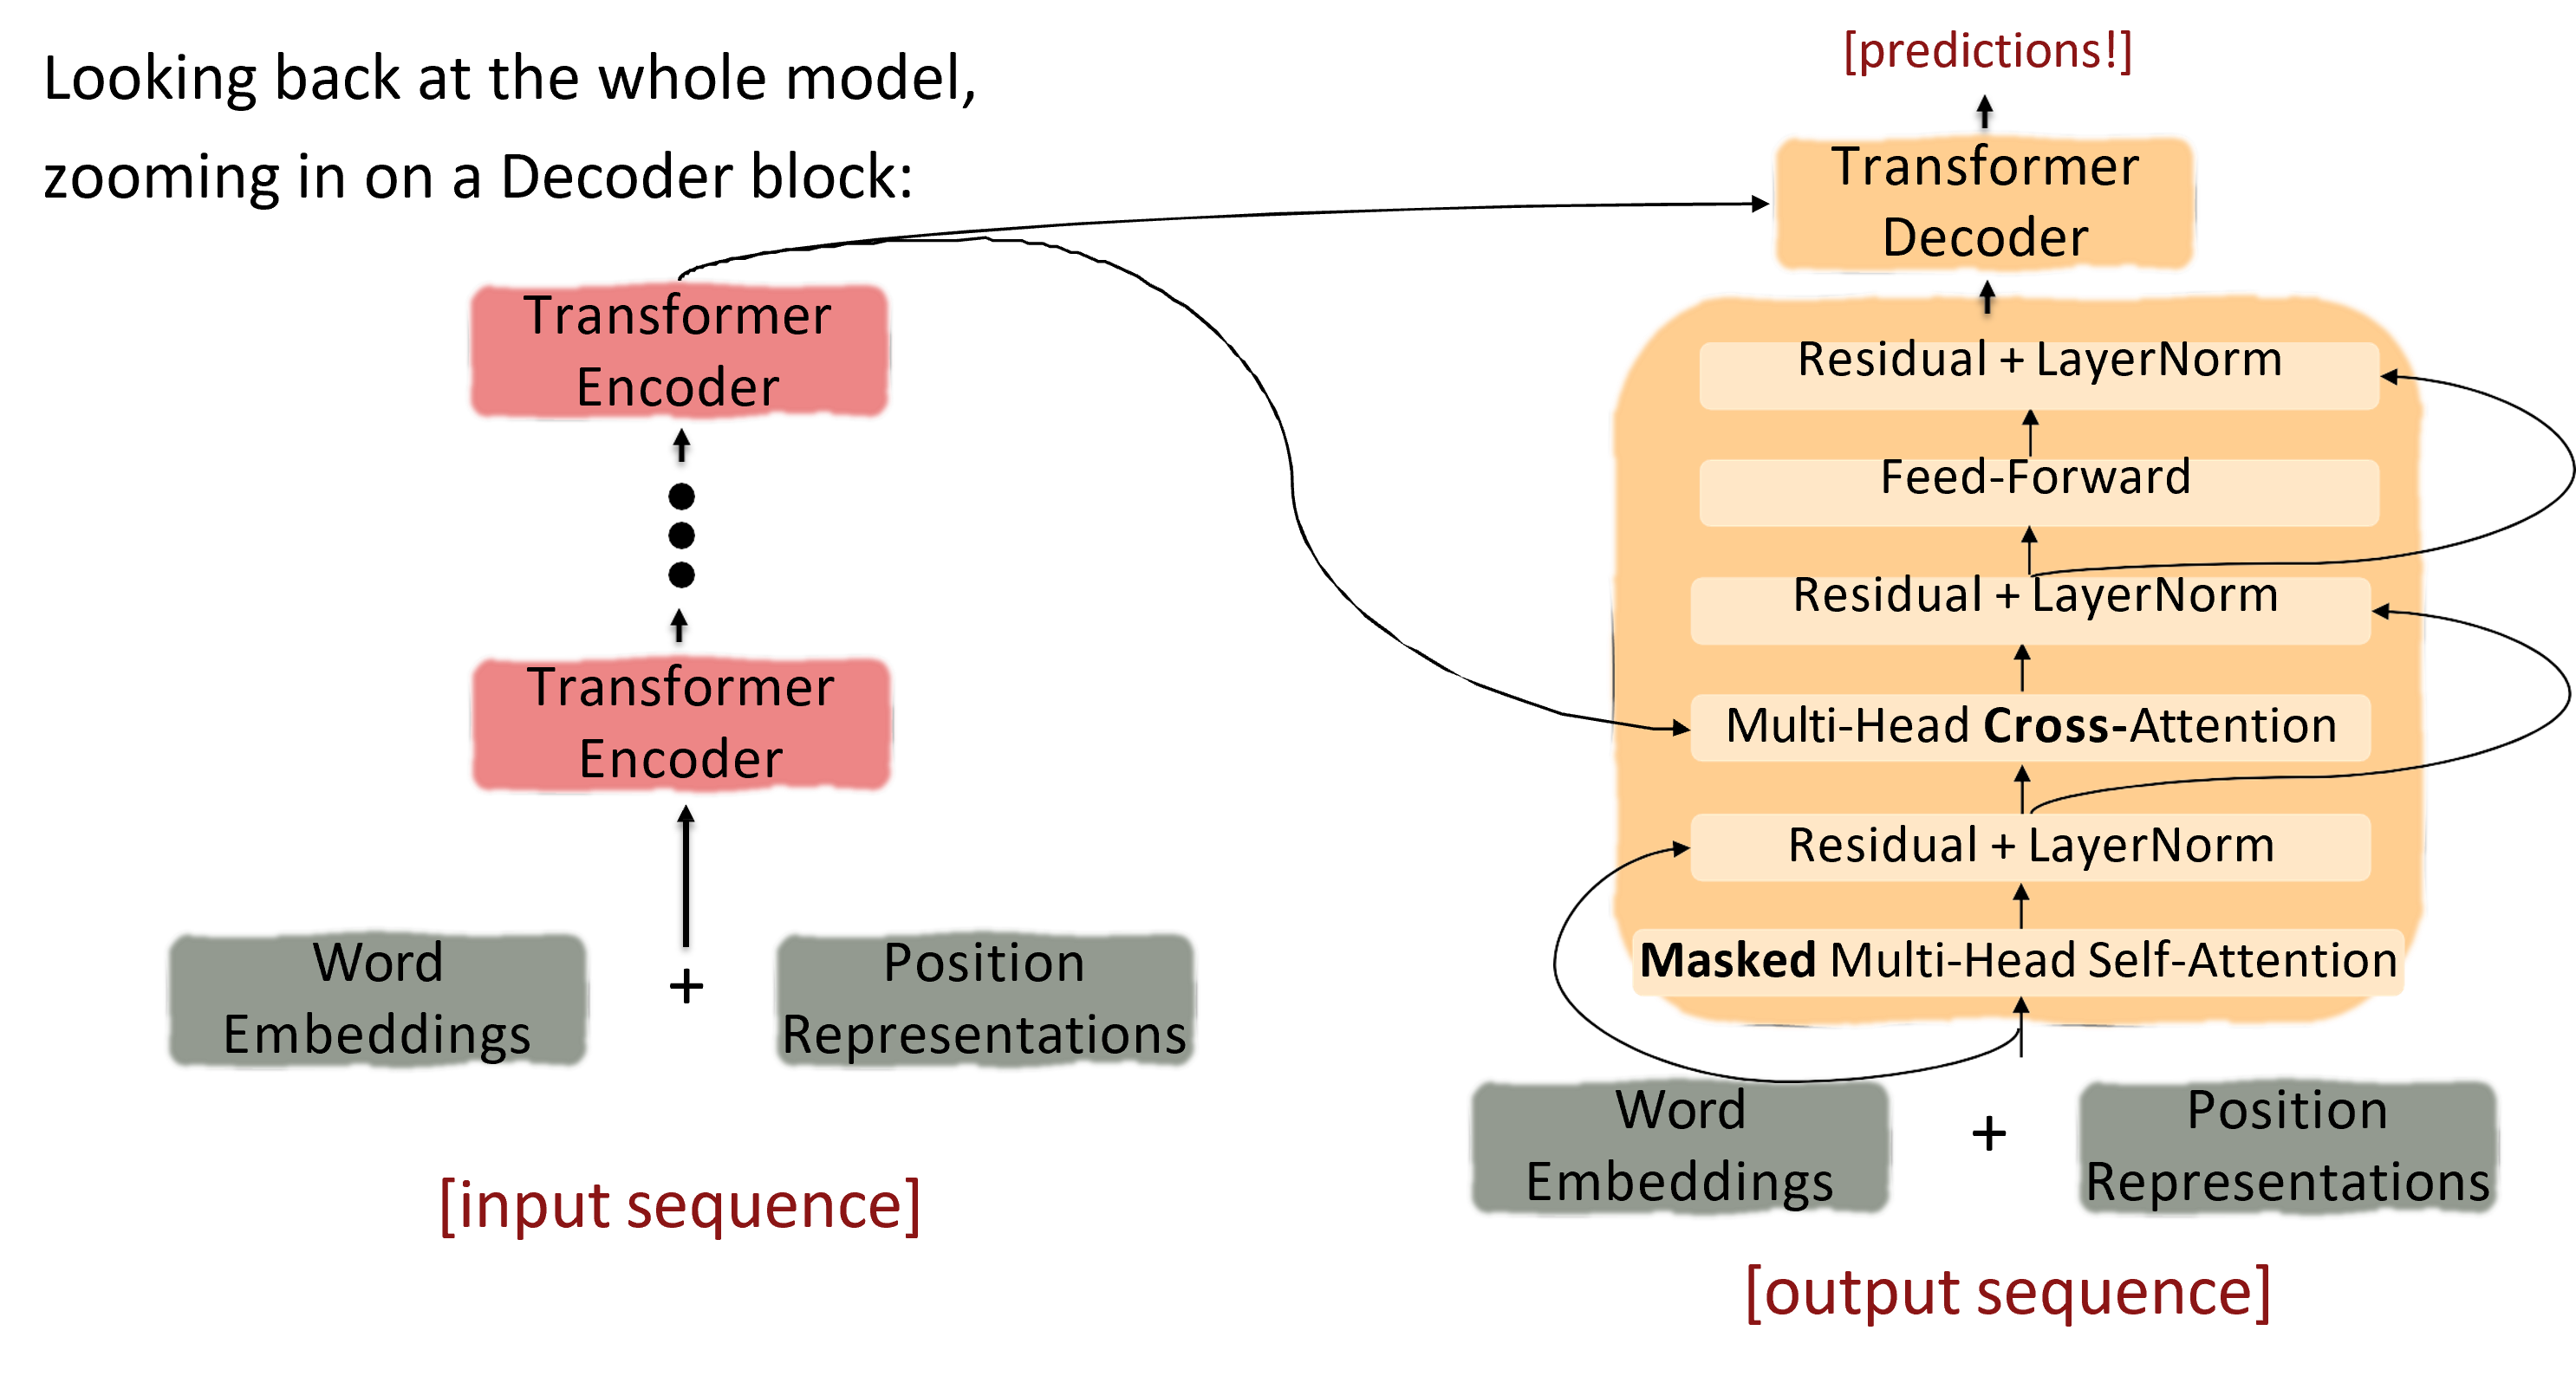
\includegraphics[width=\linewidth,keepaspectratio]{bert87}
			% \end{center}		
			
		
			% % {\tiny (Ref: John Hewitt)}

% \end{frame}

% %%%%%%%%%%%%%%%%%%%%%%%%%%%%%%%%%%%%%%%%%%%%%%%%%%%%%%%%%%%
% \begin{frame}[fragile]\frametitle{Scaled Dot Product}

						% The Transformer Encoder: Scaled Dot Product [Vaswani et al., 2017]

			
			% \begin{center}
			% 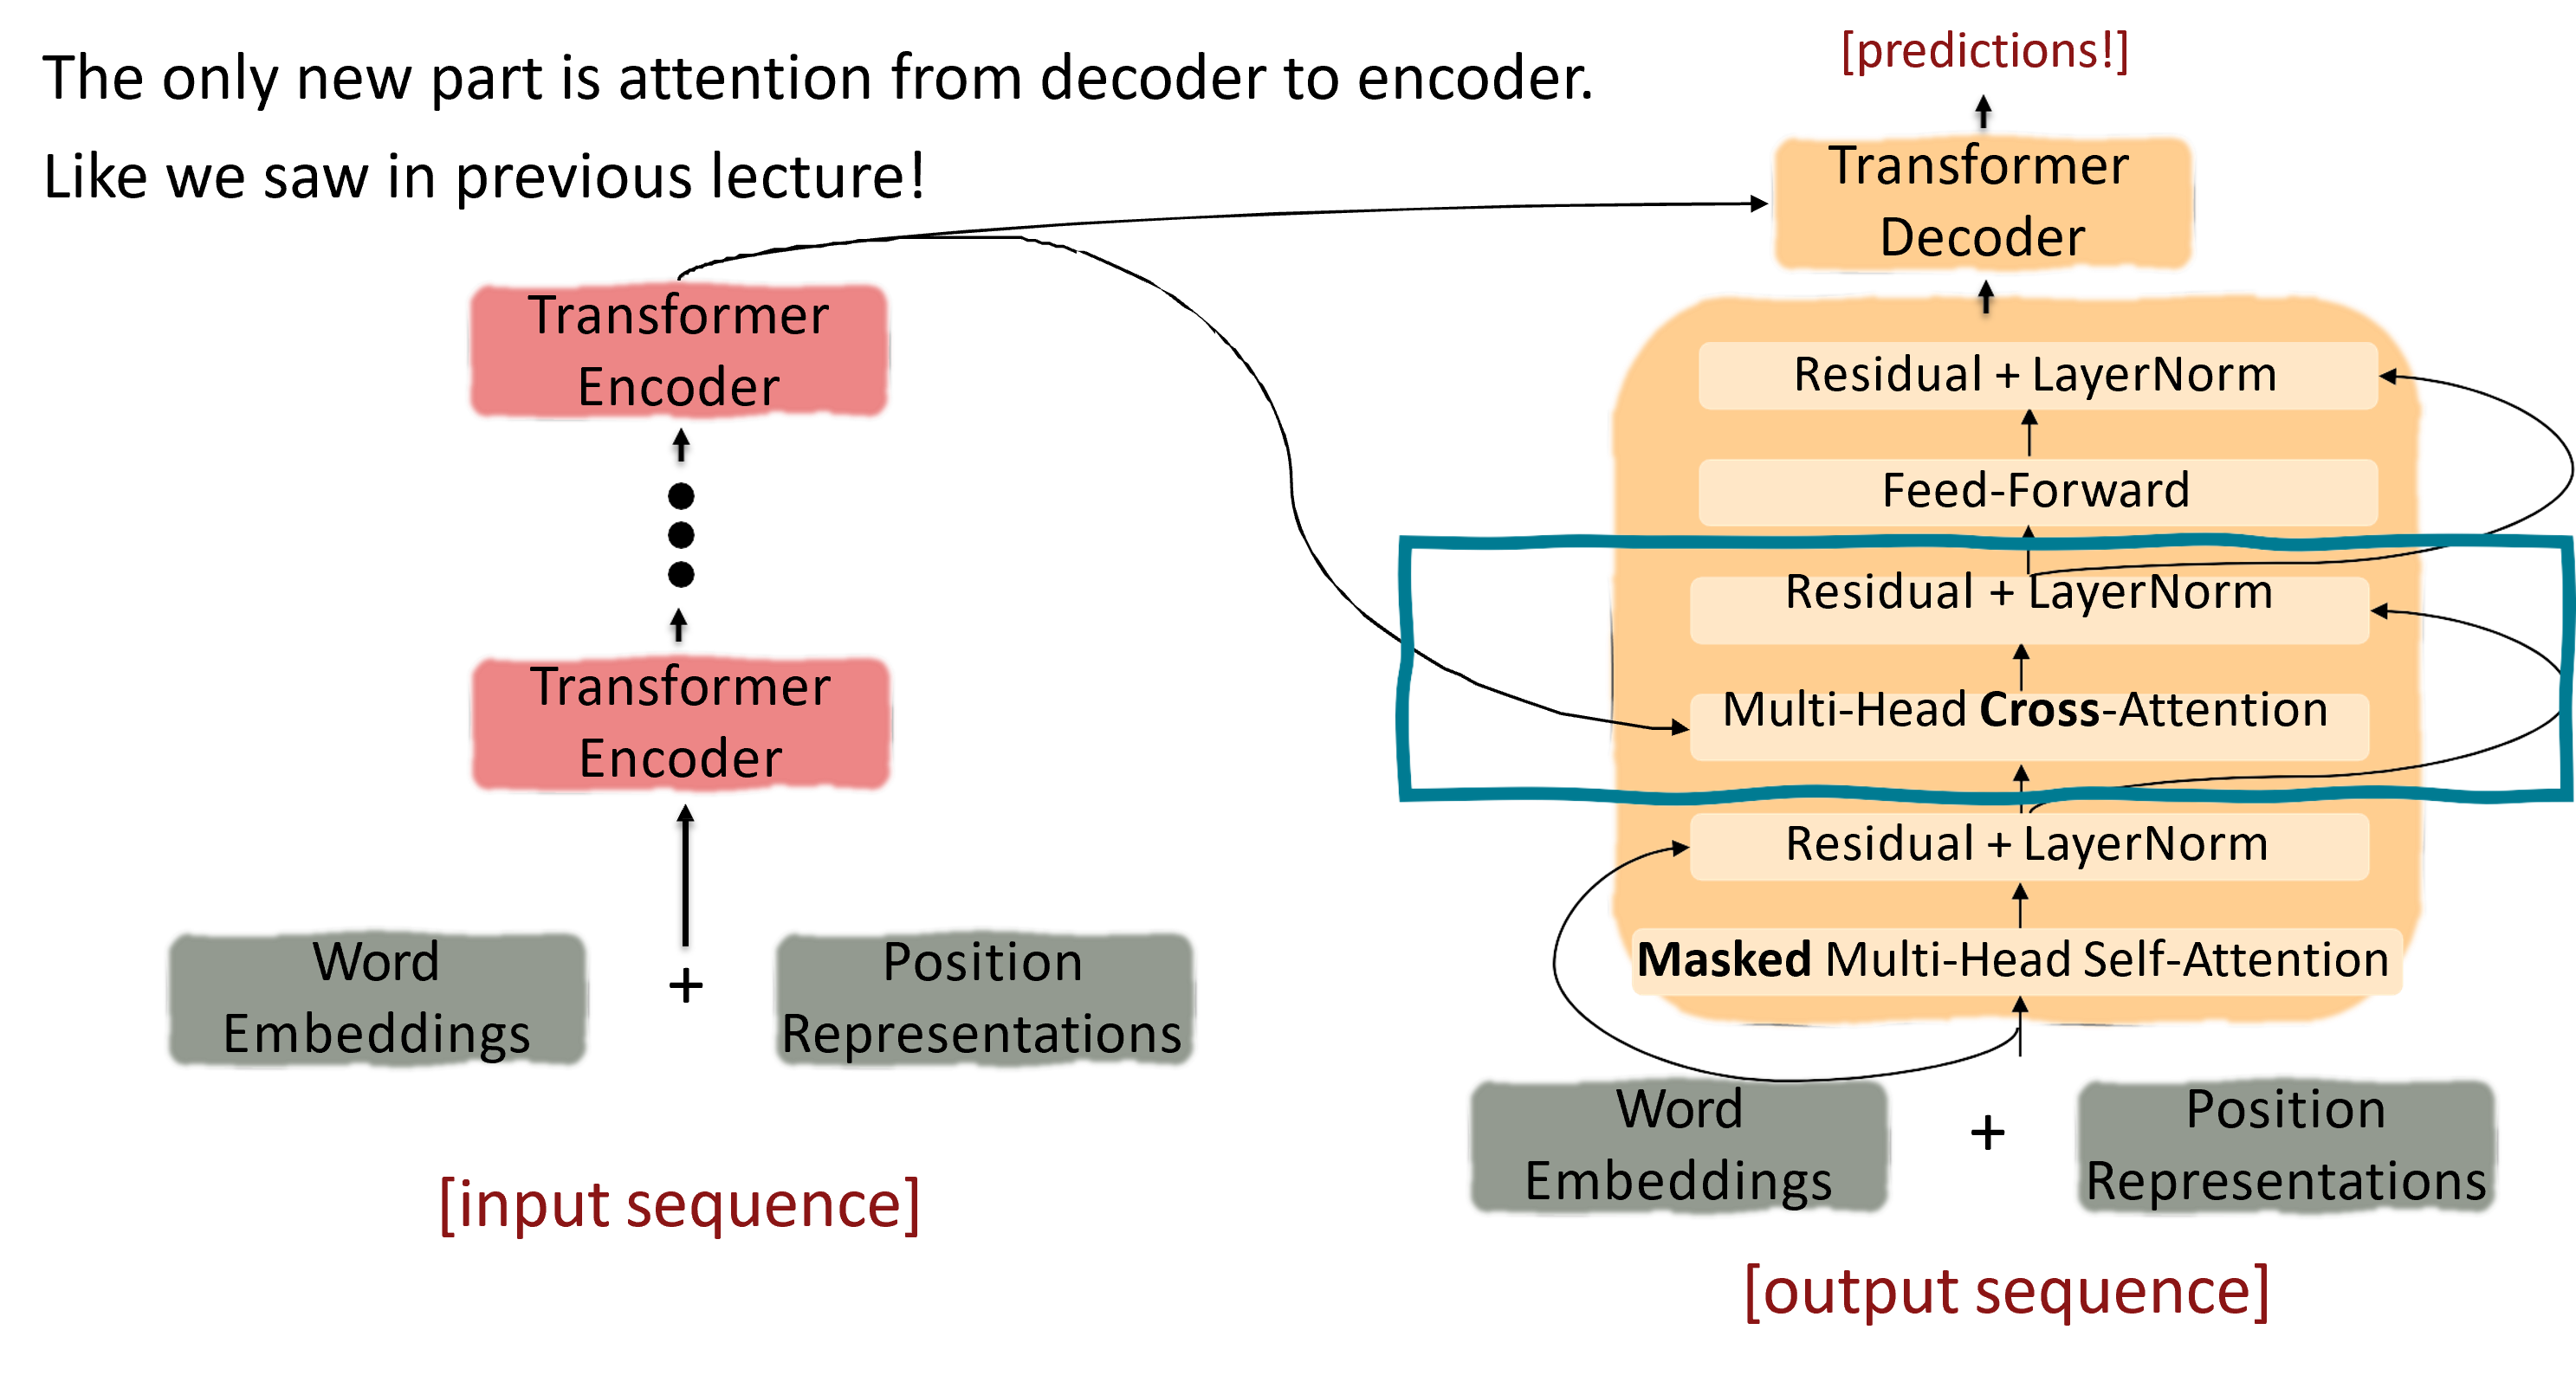
\includegraphics[width=\linewidth,keepaspectratio]{bert88}
			% \end{center}		
			
		
			% % {\tiny (Ref: John Hewitt)}

% \end{frame}

% %%%%%%%%%%%%%%%%%%%%%%%%%%%%%%%%%%%%%%%%%%%%%%%%%%%%%%%%%%%
% \begin{frame}[fragile]\frametitle{Cross-attention}

			% The Transformer Decoder: Cross-attention (details)
			
			% \begin{center}
			% 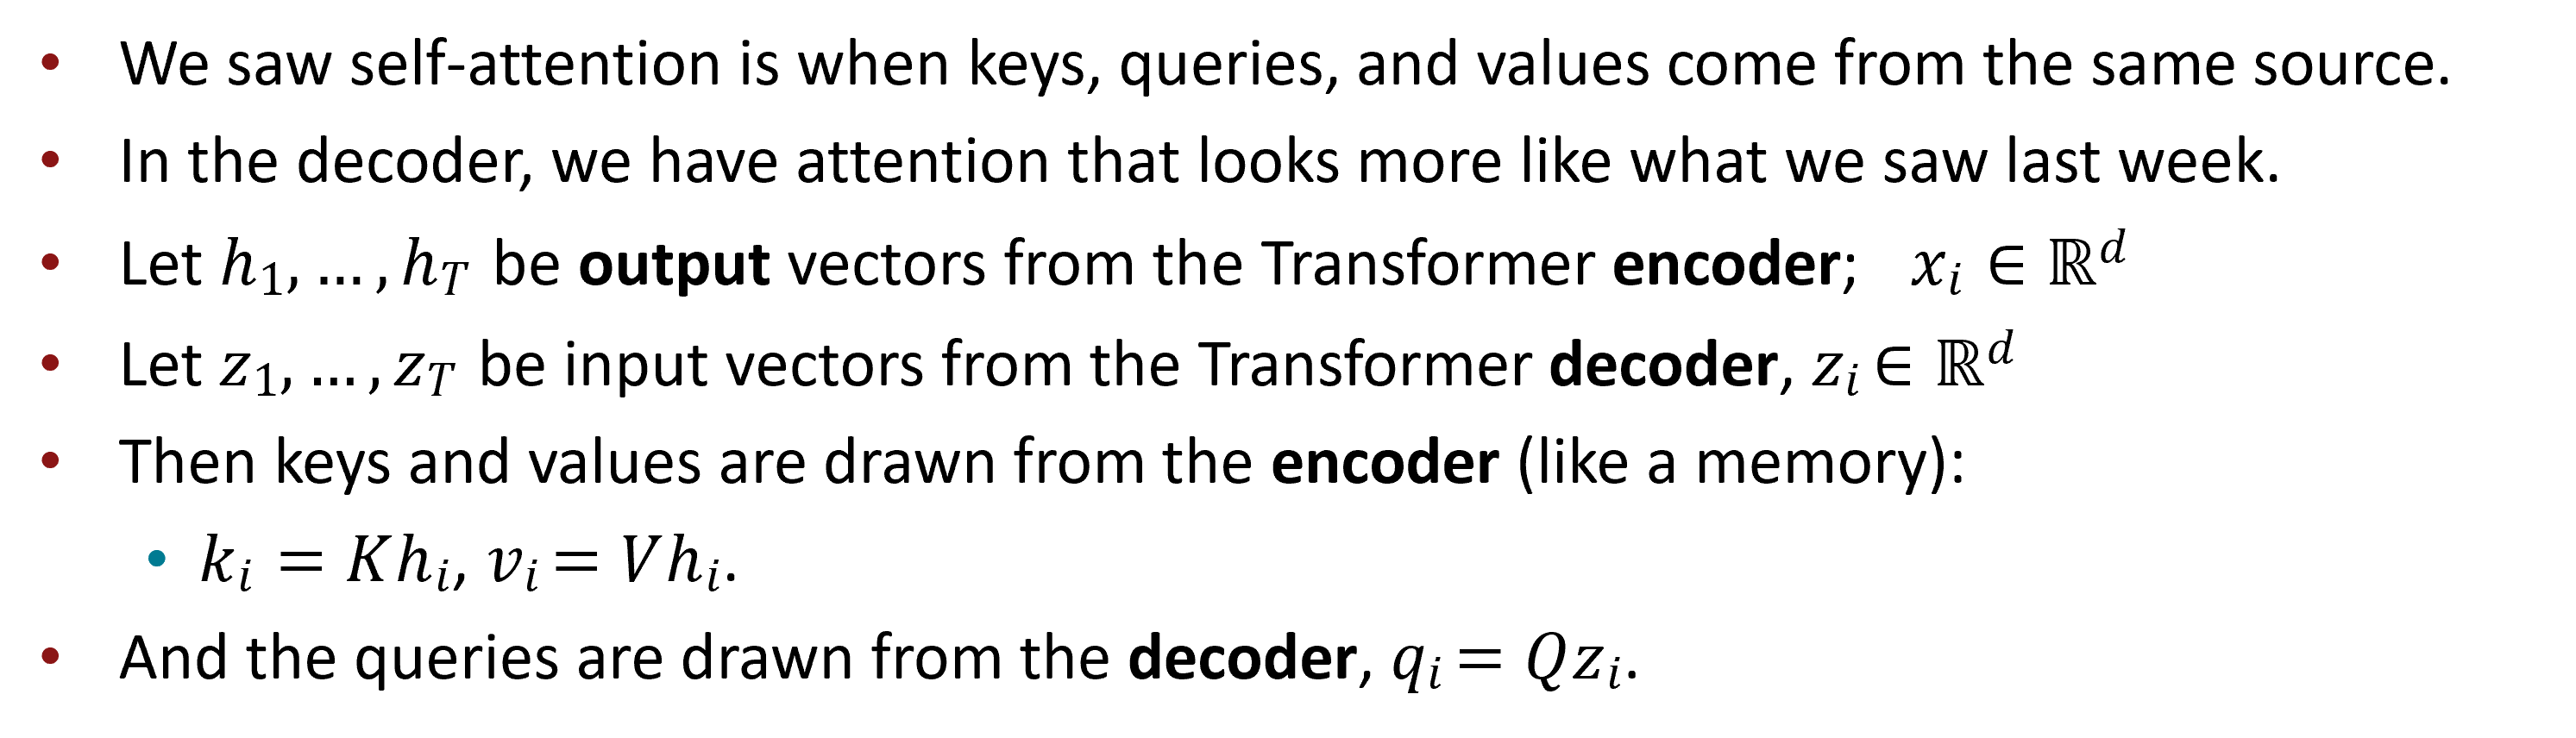
\includegraphics[width=\linewidth,keepaspectratio]{bert89}
			% \end{center}		
			
		
			% % {\tiny (Ref: John Hewitt)}

% \end{frame}

% %%%%%%%%%%%%%%%%%%%%%%%%%%%%%%%%%%%%%%%%%%%%%%%%%%%%%%%%%%%
% \begin{frame}[fragile]\frametitle{Cross-attention}

			% The Transformer Decoder: Cross-attention (details)
			
			% \begin{center}
			% 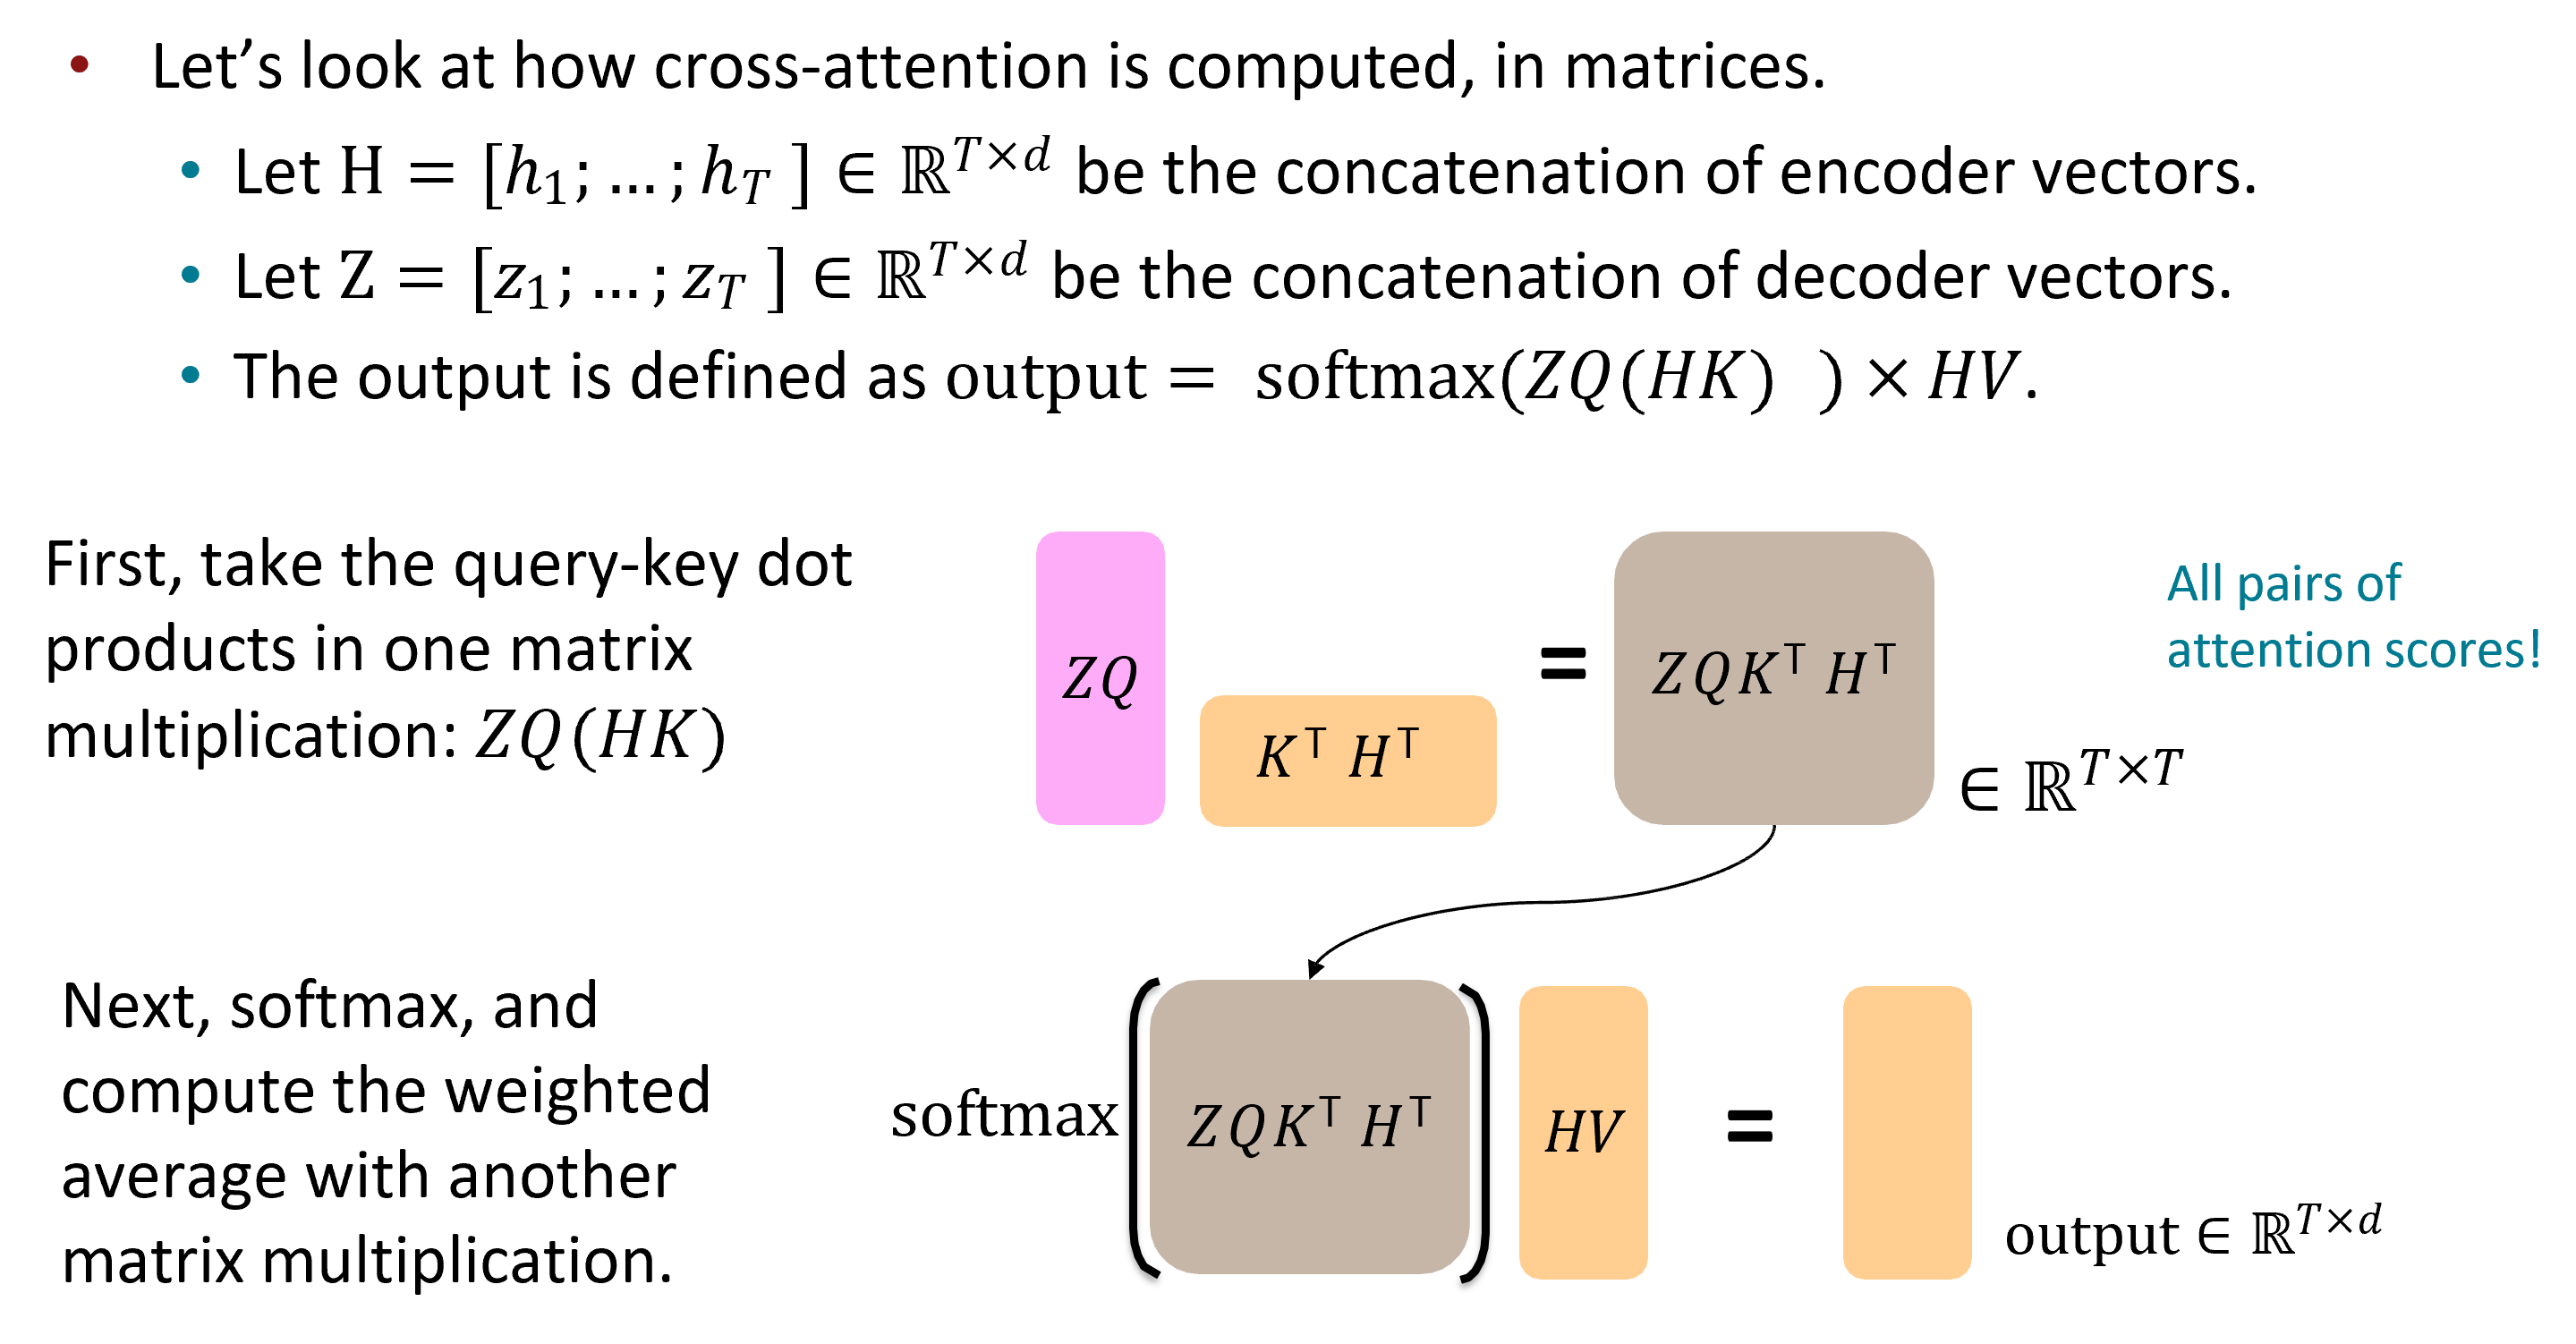
\includegraphics[width=\linewidth,keepaspectratio]{bert90}
			% \end{center}		
			
			% % {\tiny (Ref: John Hewitt)}

% \end{frame}

% %%%%%%%%%%%%%%%%%%%%%%%%%%%%%%%%%%%%%%%%%%%%%%%%%%%%%%%%%%%
% \begin{frame}[fragile]\frametitle{Results}
% Great Results with Transformers
			
			% \begin{center}
			% 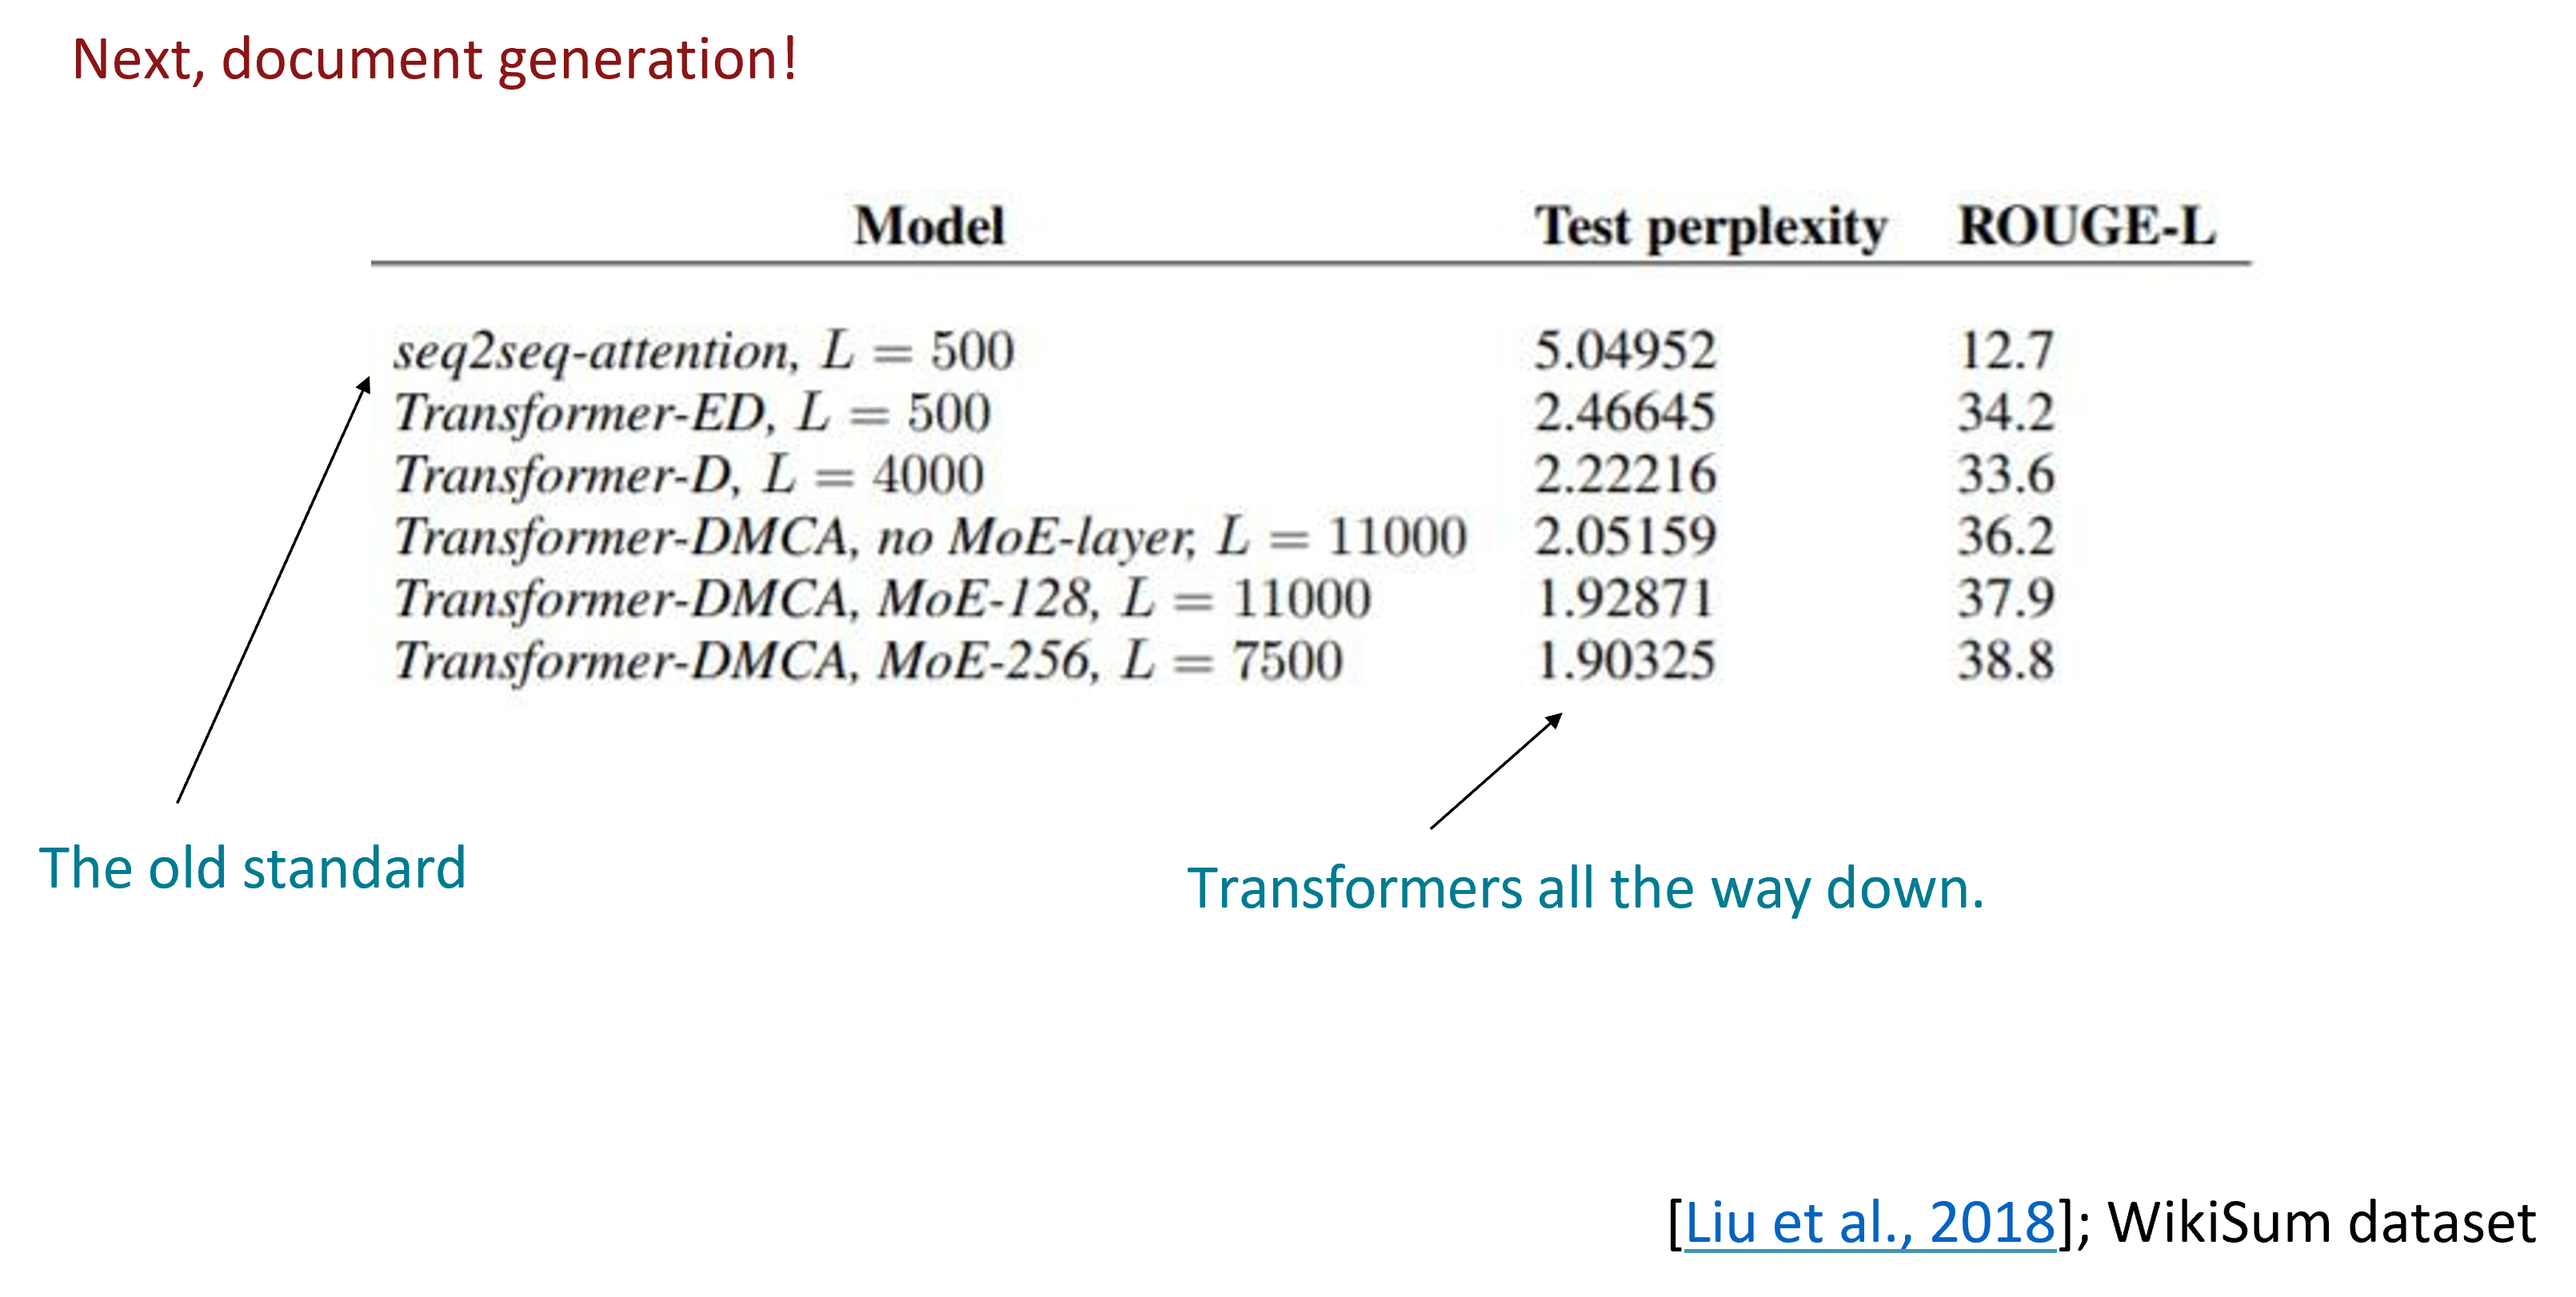
\includegraphics[width=\linewidth,keepaspectratio]{bert91}
			% \end{center}		
			
			% % {\tiny (Ref: John Hewitt)}

% \end{frame}

% %%%%%%%%%%%%%%%%%%%%%%%%%%%%%%%%%%%%%%%%%%%%%%%%%%%%%%%%%%%
% \begin{frame}[fragile]\frametitle{Issues}

% What would we like to fix about the Transformer?

      % \begin{itemize}
			% \item Quadratic compute in self-attention:
			      % \begin{itemize}
						% \item Computing all pairs of interactions means our computation grows quadratically with the sequence length!
						% \item For recurrent models, it only grew linearly!
						% \end{itemize}
			% \item Position representations:
			      % \begin{itemize}
						% \item Are simple absolute indices the best we can do to represent position?
						% \item Relative linear position attention [Shaw et al., 2018]
						% \item Dependency syntax-based position [Wang et al., 2019]			
						% \end{itemize}
			% \end{itemize}

			% % {\tiny (Ref: John Hewitt)}

% \end{frame}

% %%%%%%%%%%%%%%%%%%%%%%%%%%%%%%%%%%%%%%%%%%%%%%%%%%%%%%%%%%%
% \begin{frame}[fragile]\frametitle{Quadratic computation as function of seq. length}

			
			% \begin{center}
			% 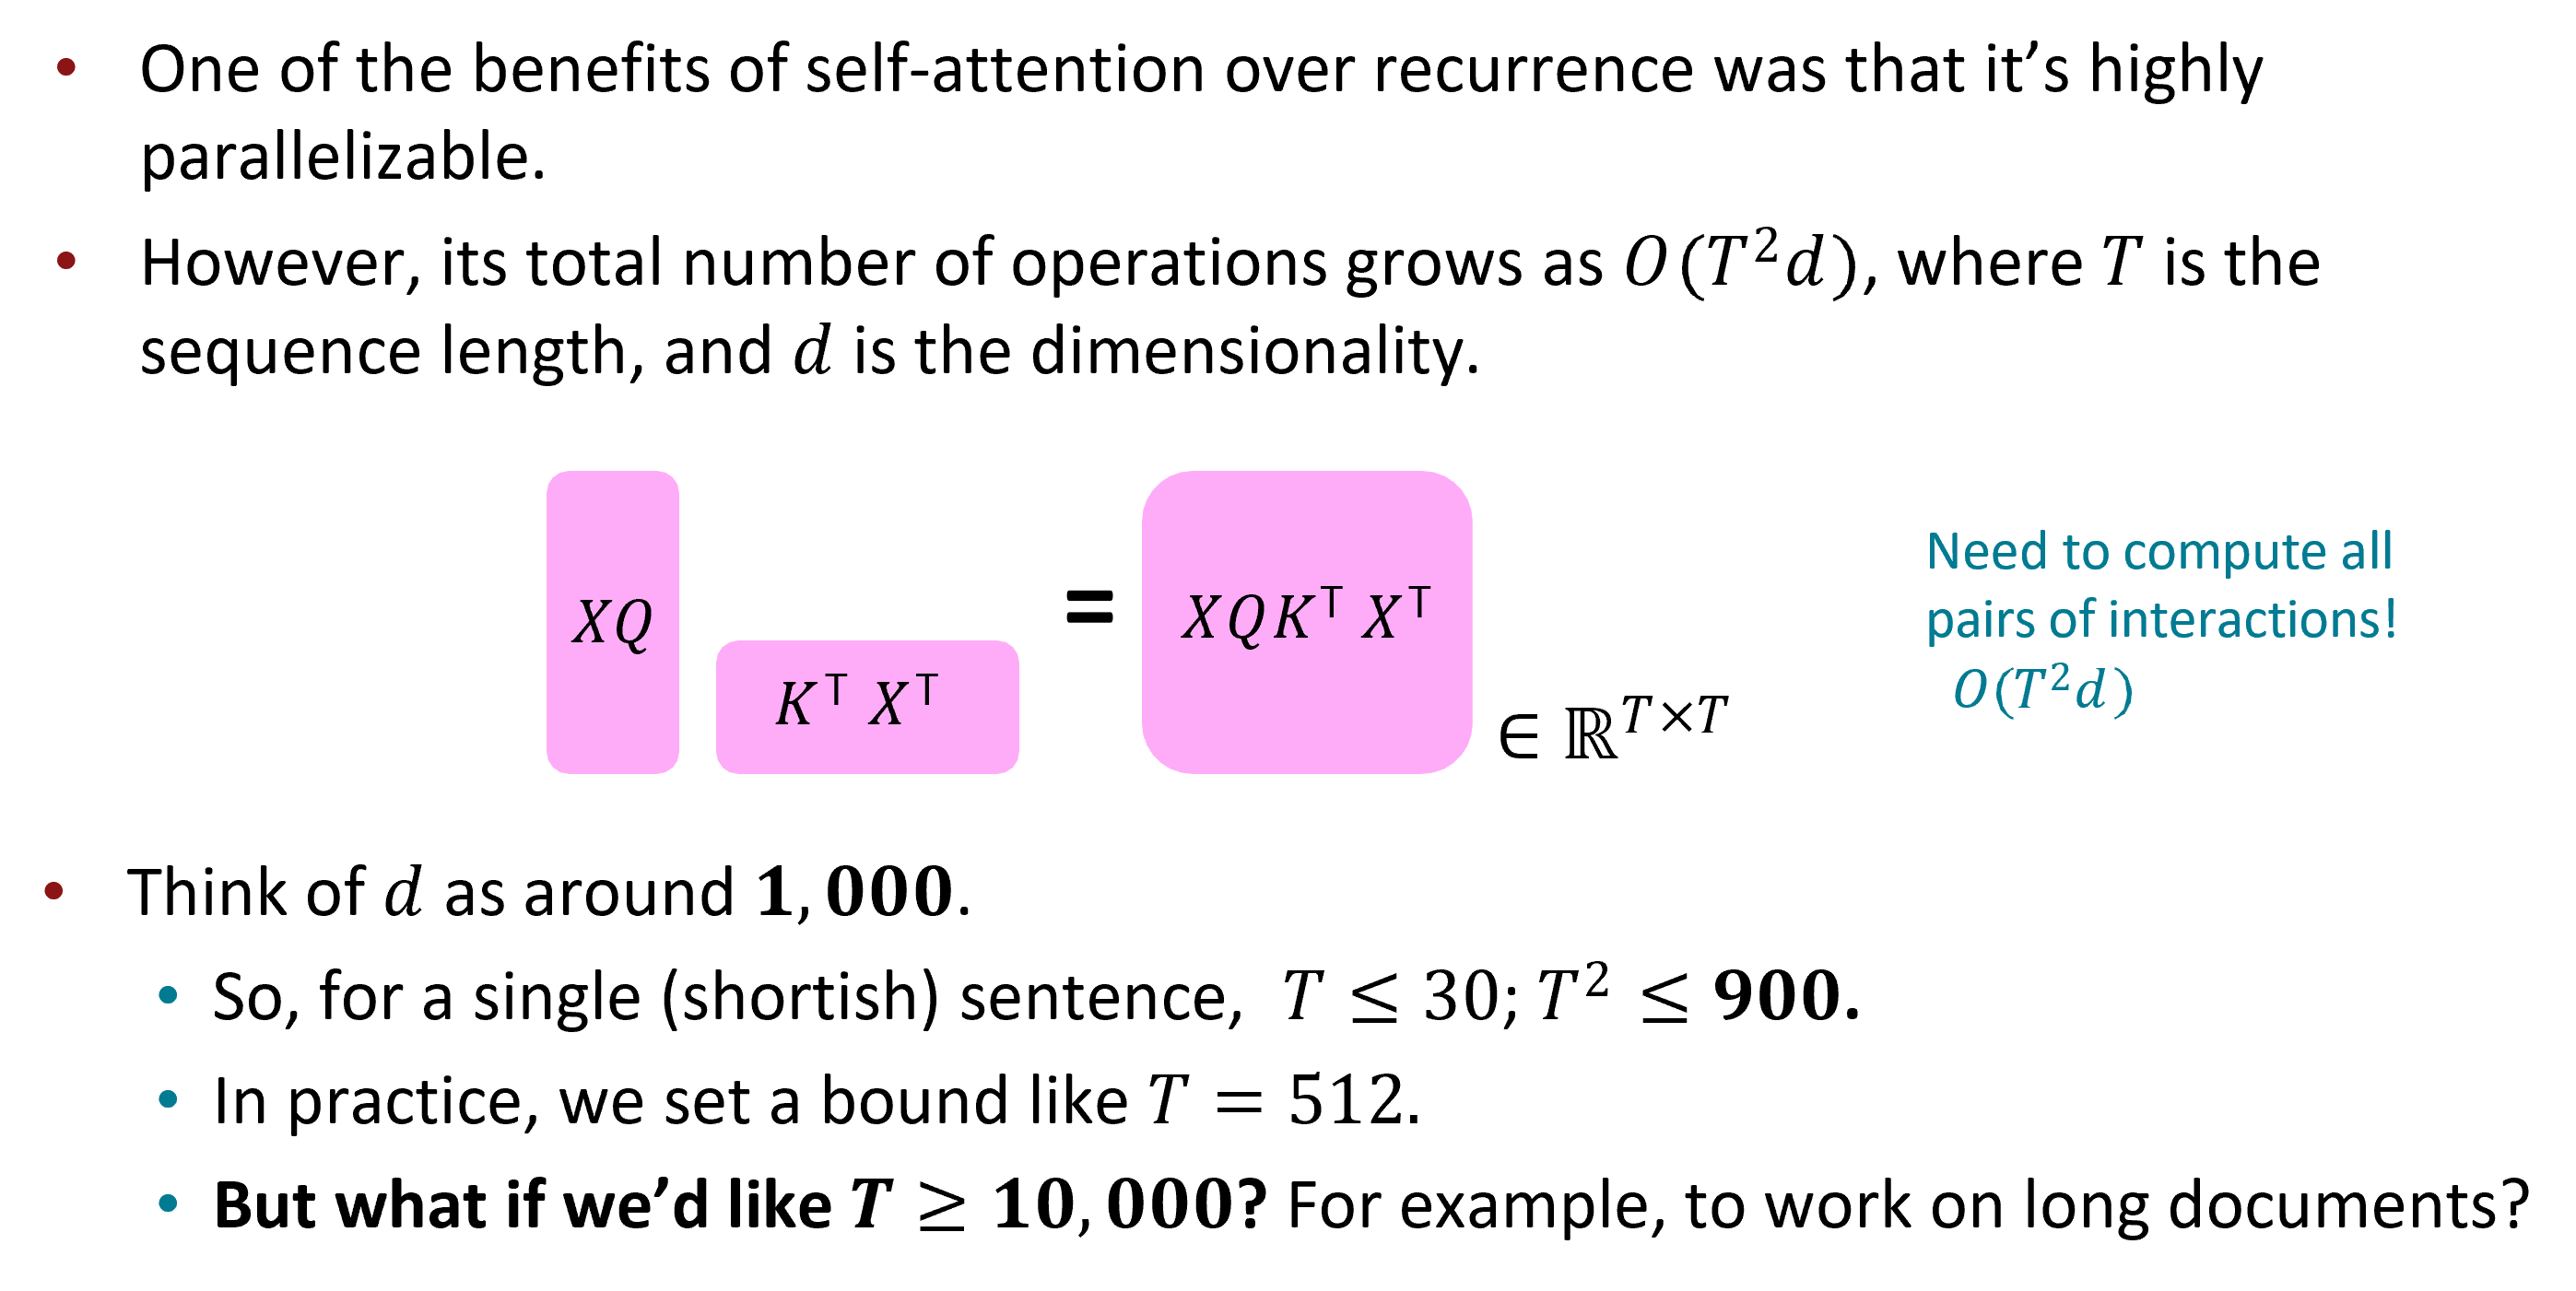
\includegraphics[width=\linewidth,keepaspectratio]{bert92}
			% \end{center}		
			
			% % {\tiny (Ref: John Hewitt)}

% \end{frame}

% %%%%%%%%%%%%%%%%%%%%%%%%%%%%%%%%%%%%%%%%%%%%%%%%%%%%%%%%%%%
% \begin{frame}[fragile]\frametitle{Recent work on improving on quadratic self-attention cost}

			
			% \begin{center}
			% 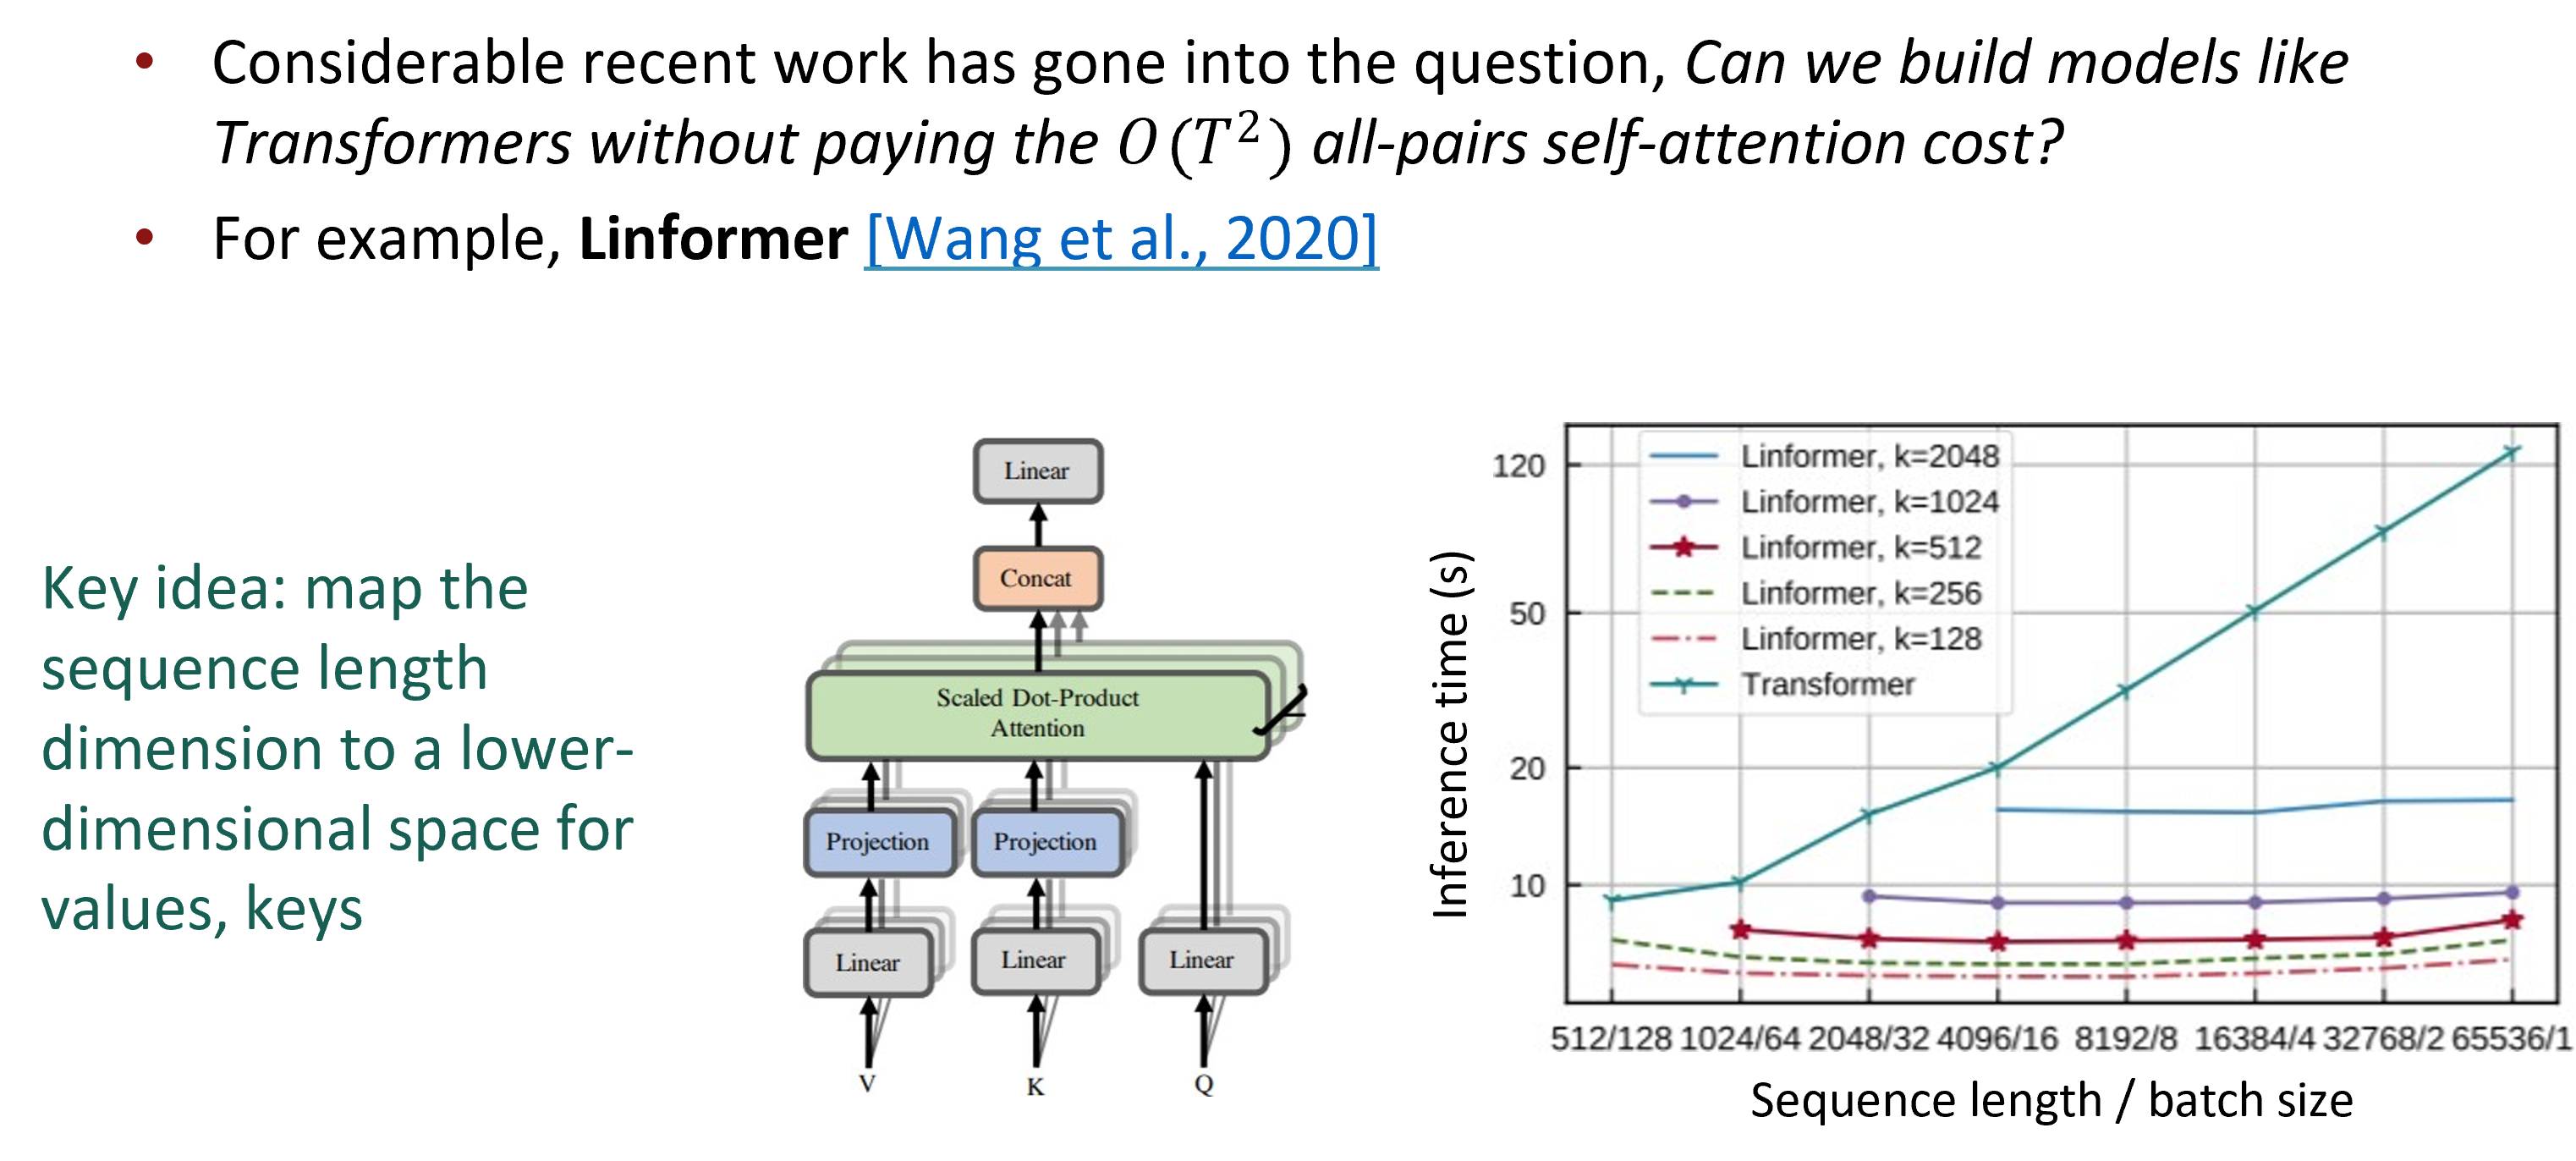
\includegraphics[width=\linewidth,keepaspectratio]{bert93}
			% \end{center}		
			
			% % {\tiny (Ref: John Hewitt)}

% \end{frame}

% %%%%%%%%%%%%%%%%%%%%%%%%%%%%%%%%%%%%%%%%%%%%%%%%%%%%%%%%%%%
% \begin{frame}[fragile]\frametitle{Recent work on improving on quadratic self-attention cost}

			
			% \begin{center}
			% 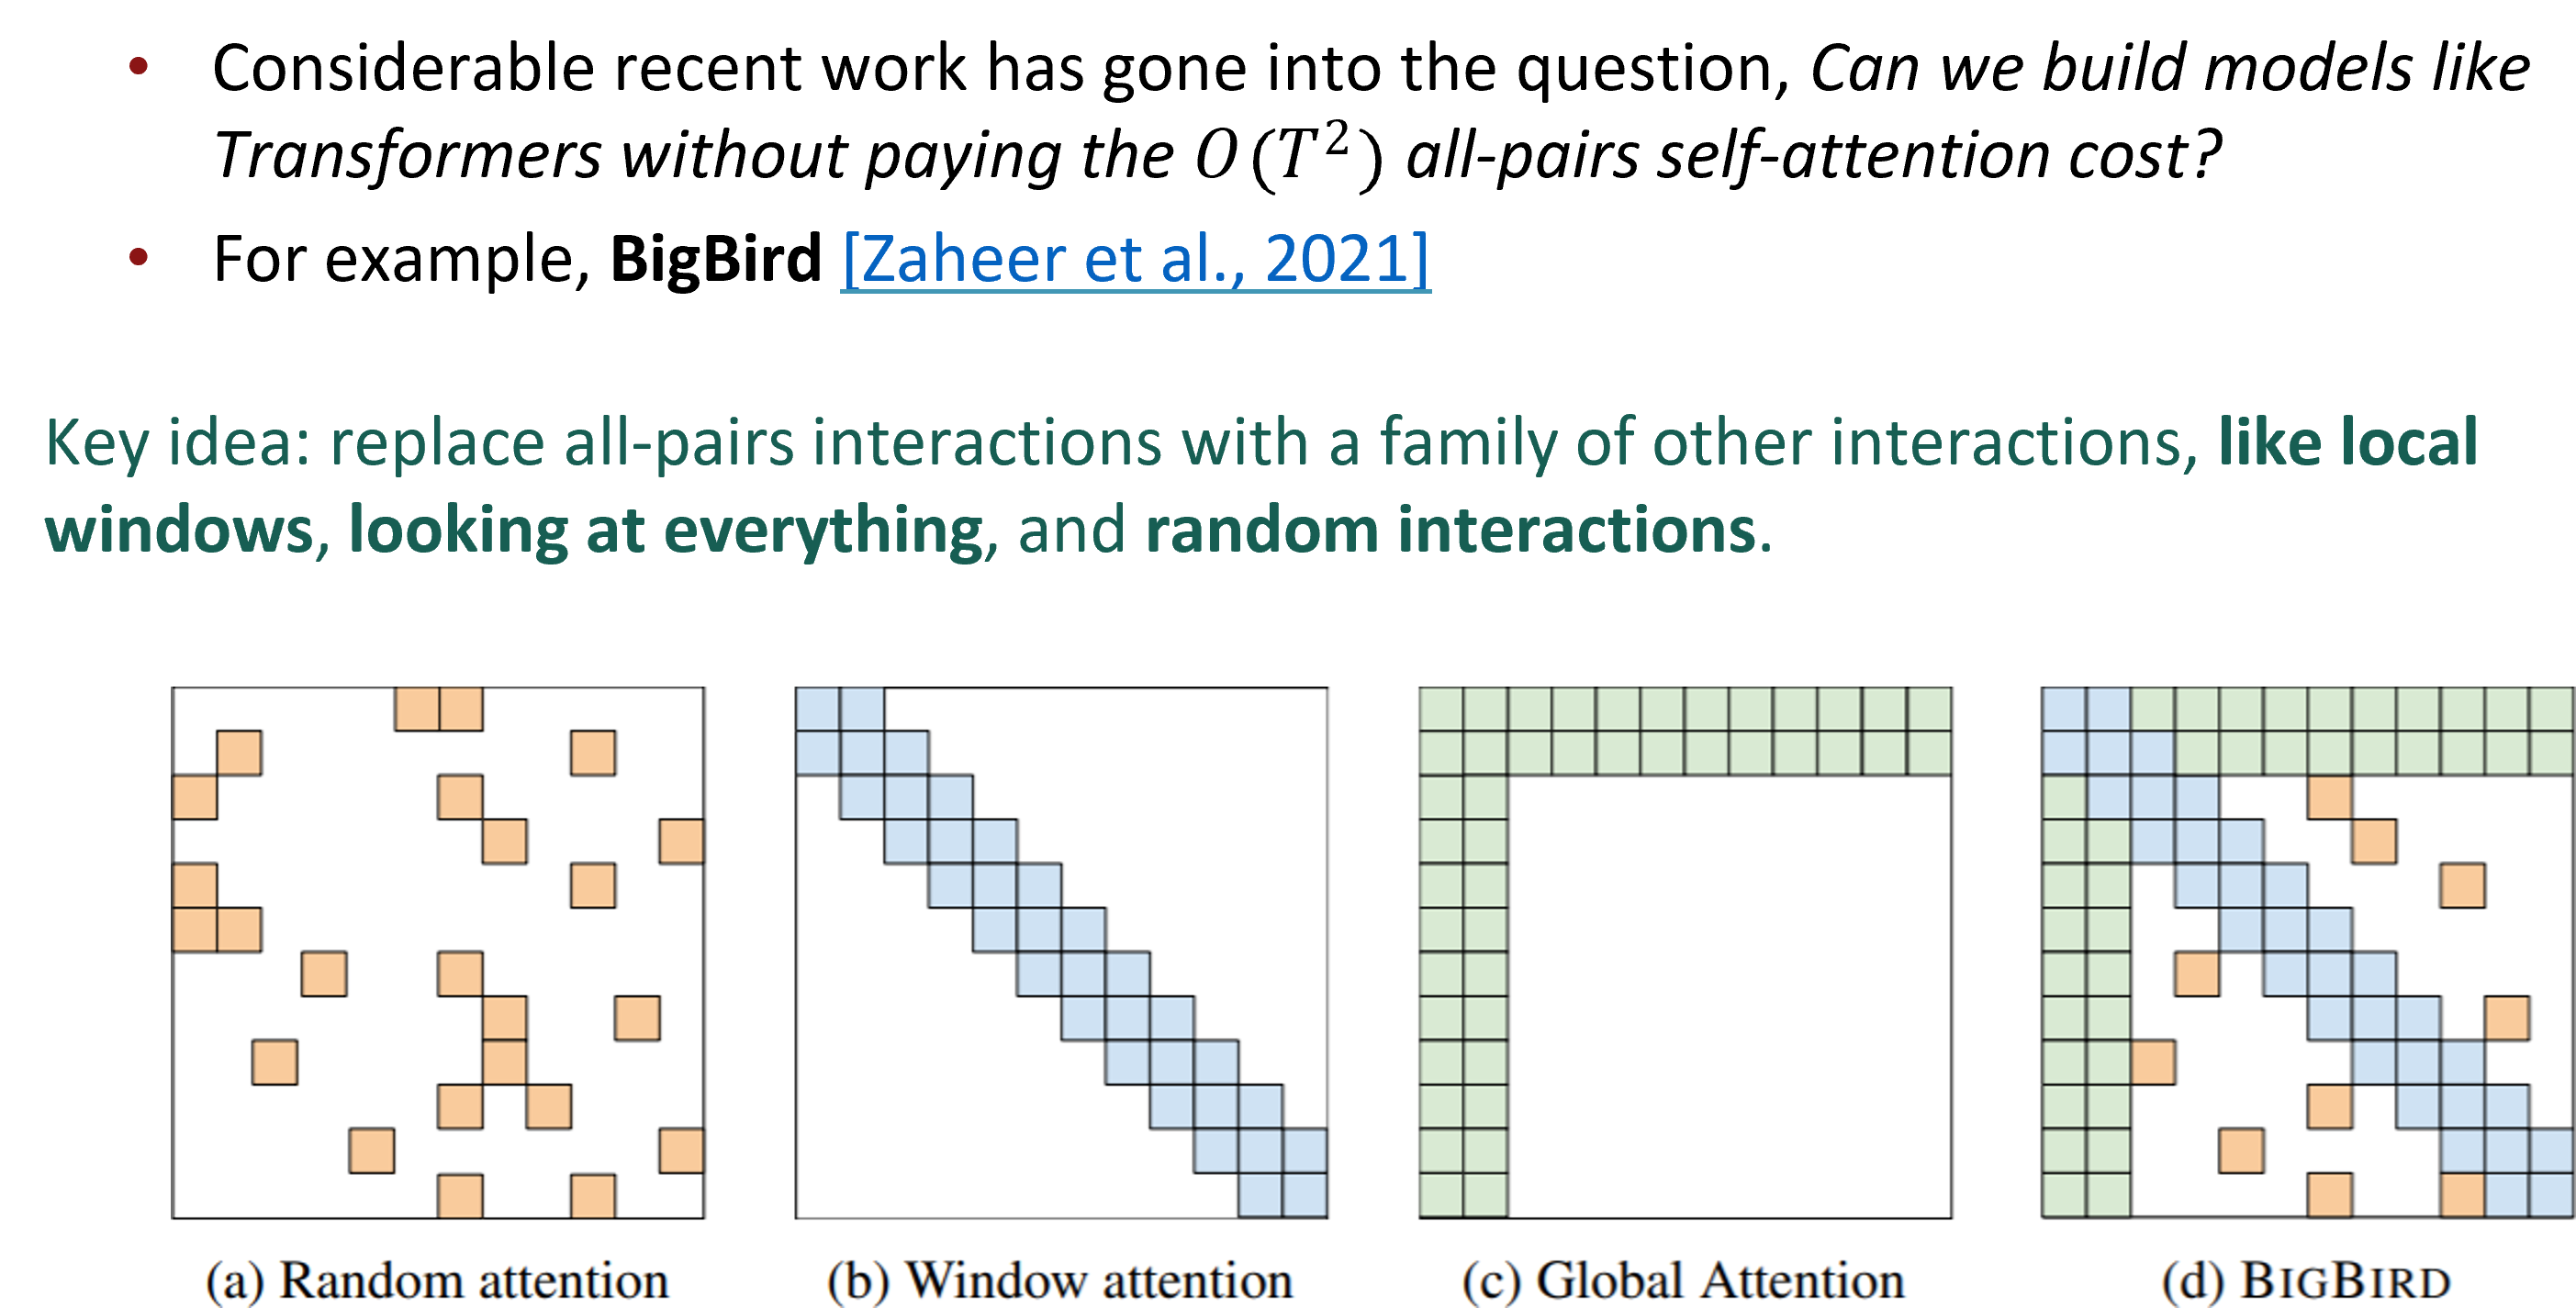
\includegraphics[width=\linewidth,keepaspectratio]{bert94}
			% \end{center}		
			
			% % {\tiny (Ref: John Hewitt)}

% \end{frame}

% %%%%%%%%%%%%%%%%%%%%%%%%%%%%%%%%%%%%%%%%%%%%%%%%%%%%%%%%%%%
% \begin{frame}[fragile]\frametitle{Recent work on improving on quadratic self-attention cost}

			
			% \begin{center}
			% 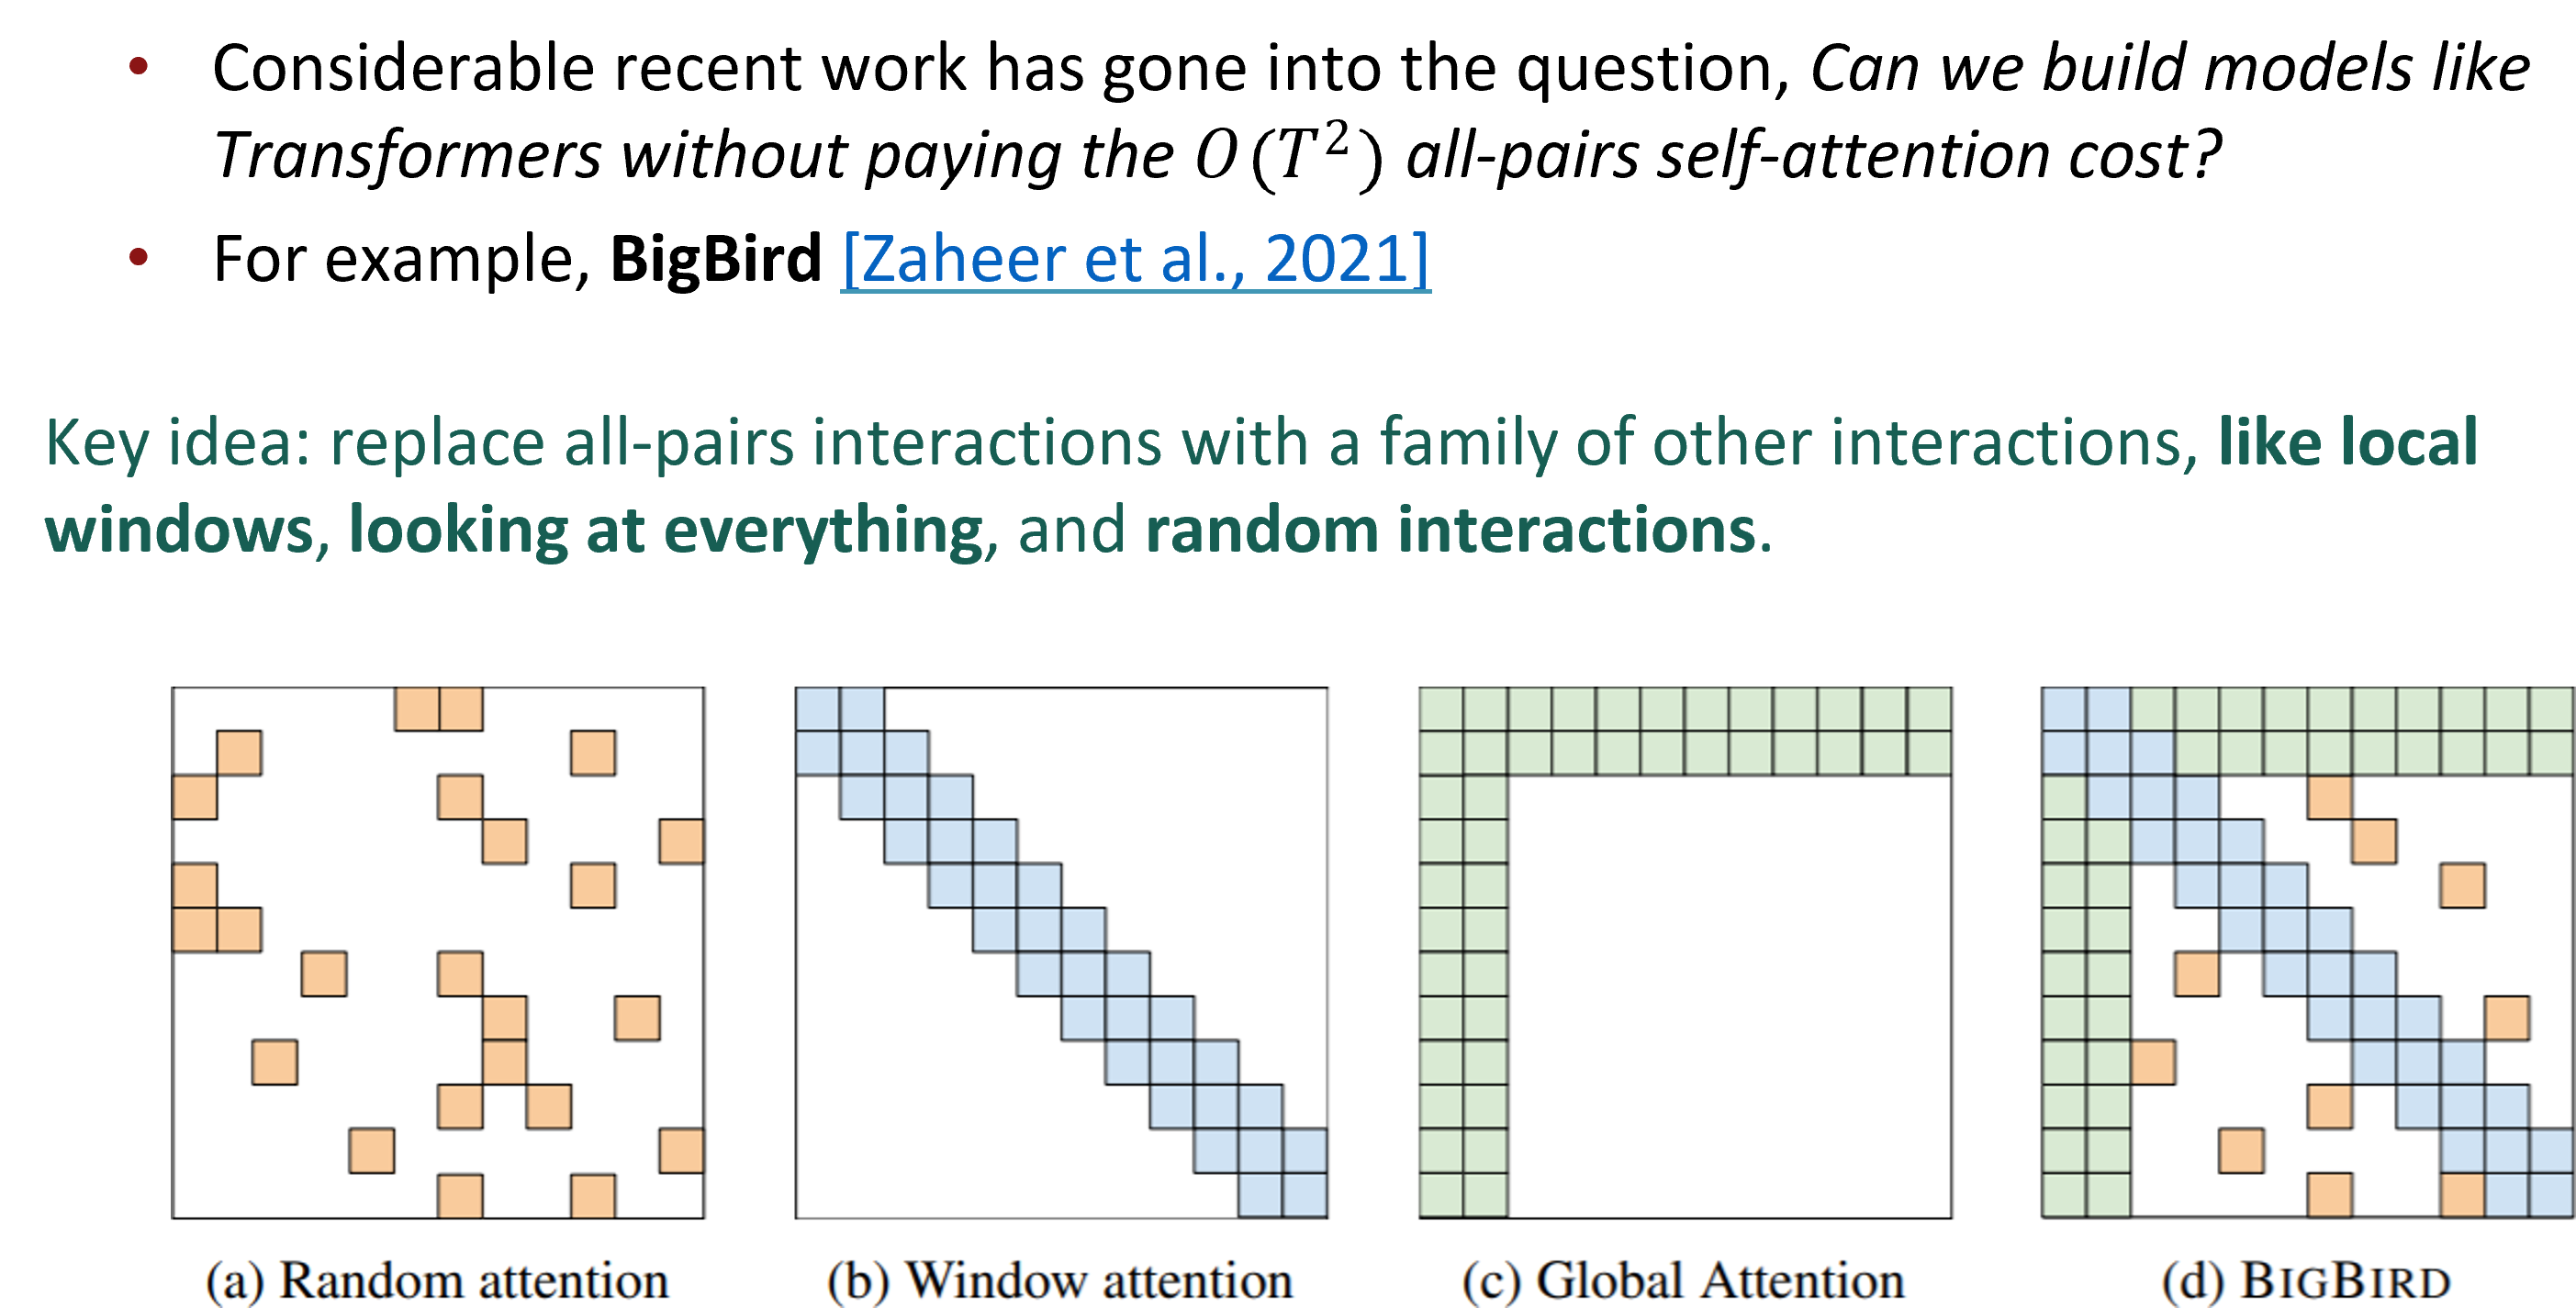
\includegraphics[width=\linewidth,keepaspectratio]{bert95}
			% \end{center}		
			
			% % {\tiny (Ref: John Hewitt)}

% \end{frame}

% %%%%%%%%%%%%%%%%%%%%%%%%%%%%%%%%%%%%%%%%%%%%%%%%%%%%%%%%%%%%%%%%%%%%%%%%%%%%%%%%%%
% \begin{frame}[fragile]\frametitle{}
% \begin{center}
% {\Large Pretraining models}
% \end{center}
% \end{frame}


% %%%%%%%%%%%%%%%%%%%%%%%%%%%%%%%%%%%%%%%%%%%%%%%%%%%%%%%%%%%
% \begin{frame}[fragile]\frametitle{Introduction}

			
			% \begin{center}
			% 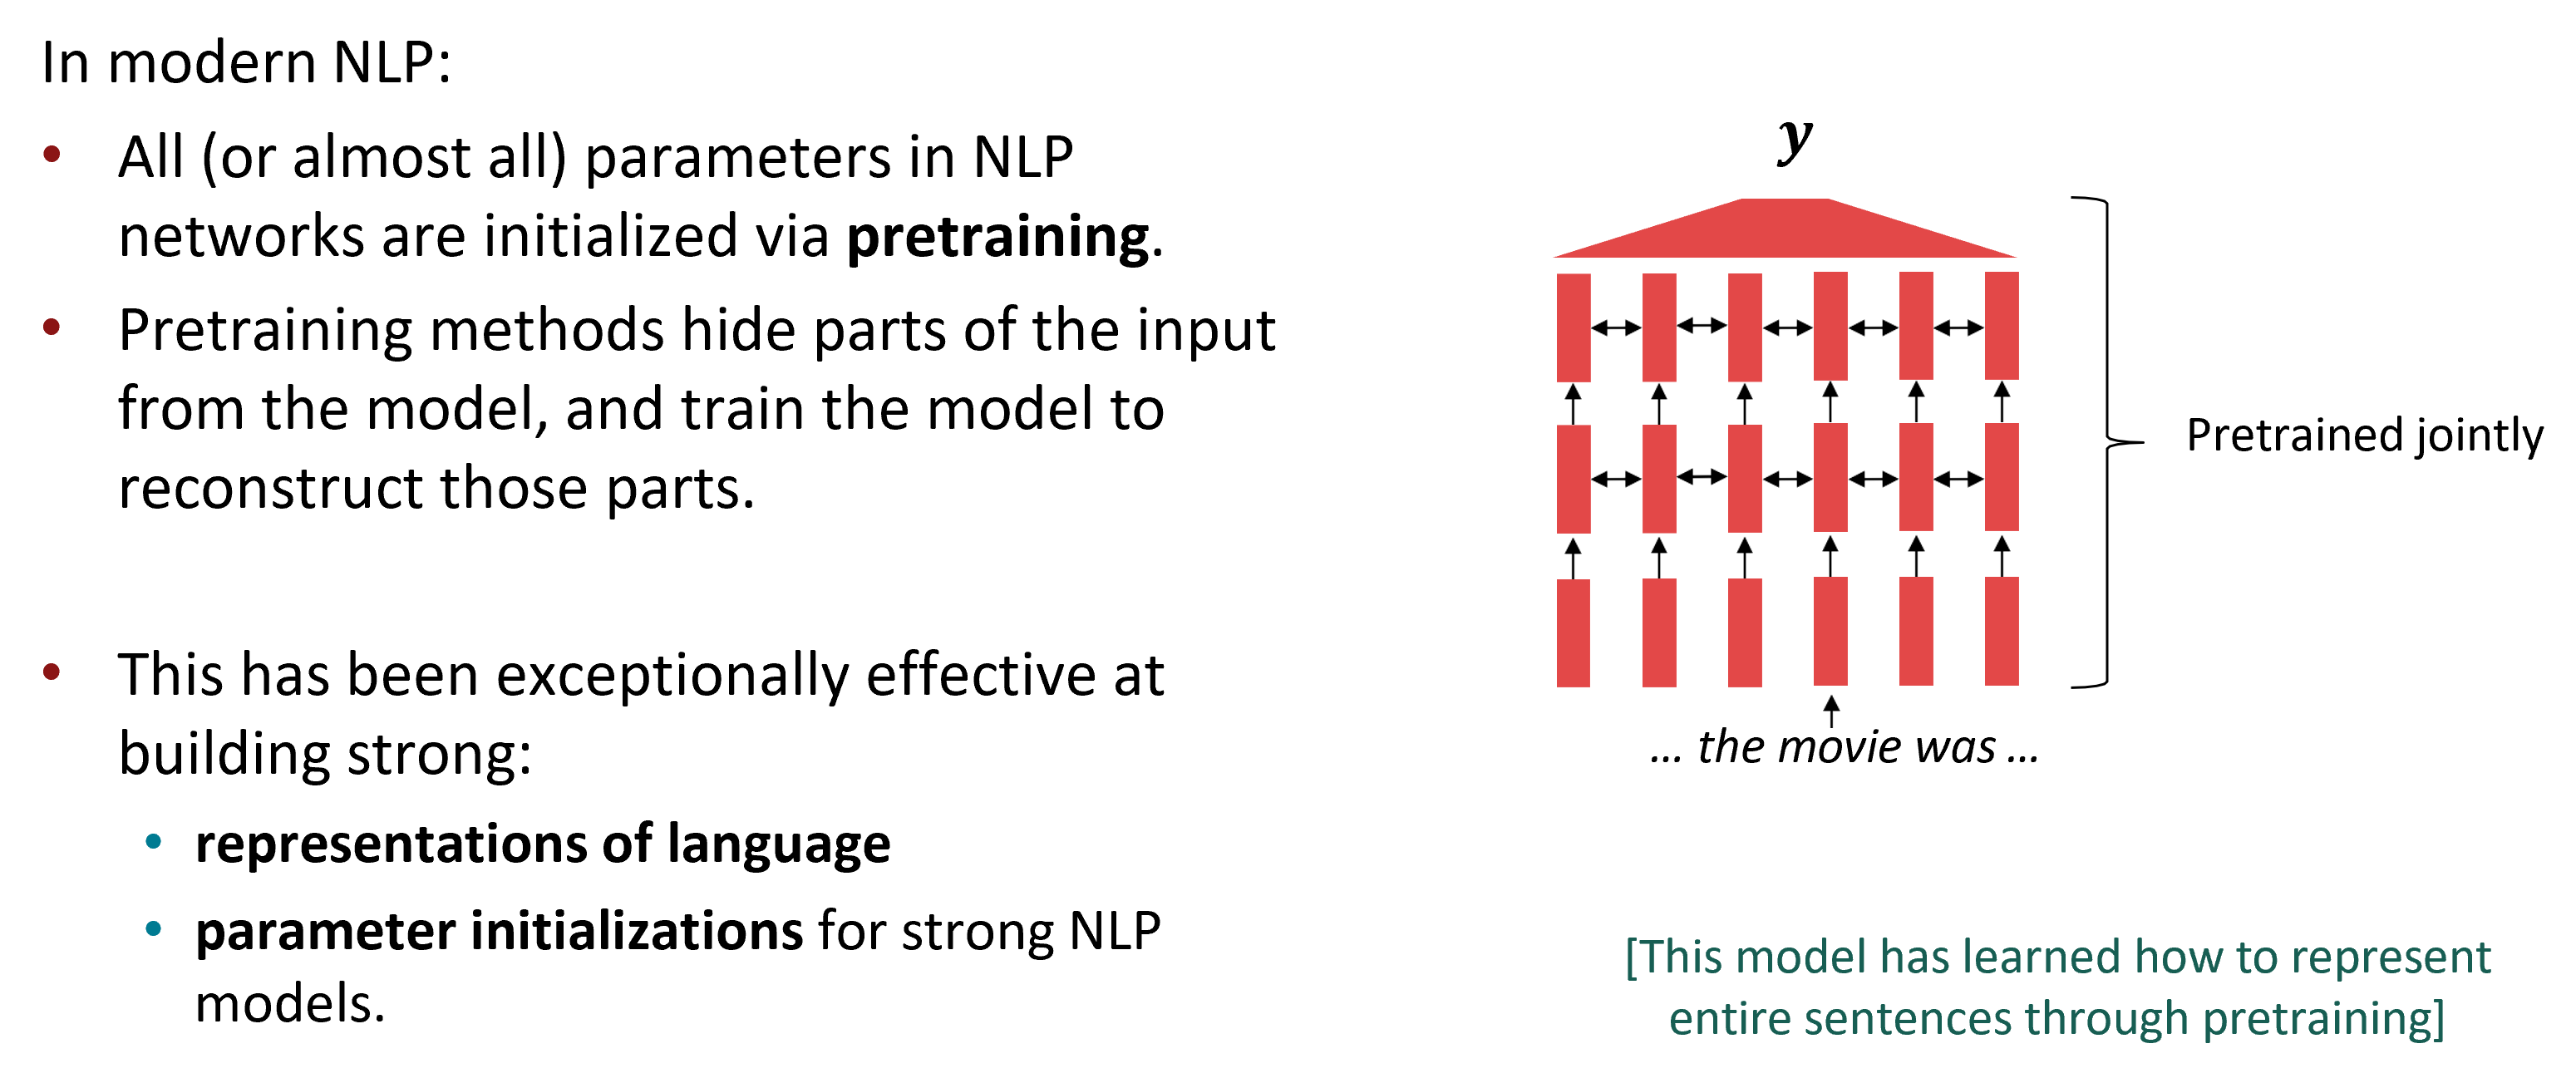
\includegraphics[width=\linewidth,keepaspectratio]{bert96}
			% \end{center}		
			
			% % {\tiny (Ref: John Hewitt)}

% \end{frame}

% %%%%%%%%%%%%%%%%%%%%%%%%%%%%%%%%%%%%%%%%%%%%%%%%%%%%%%%%%%%
% \begin{frame}[fragile]\frametitle{Pretraining models}
% Pretraining through language modeling [Dai and Le, 2015]
			
			% \begin{center}
			% 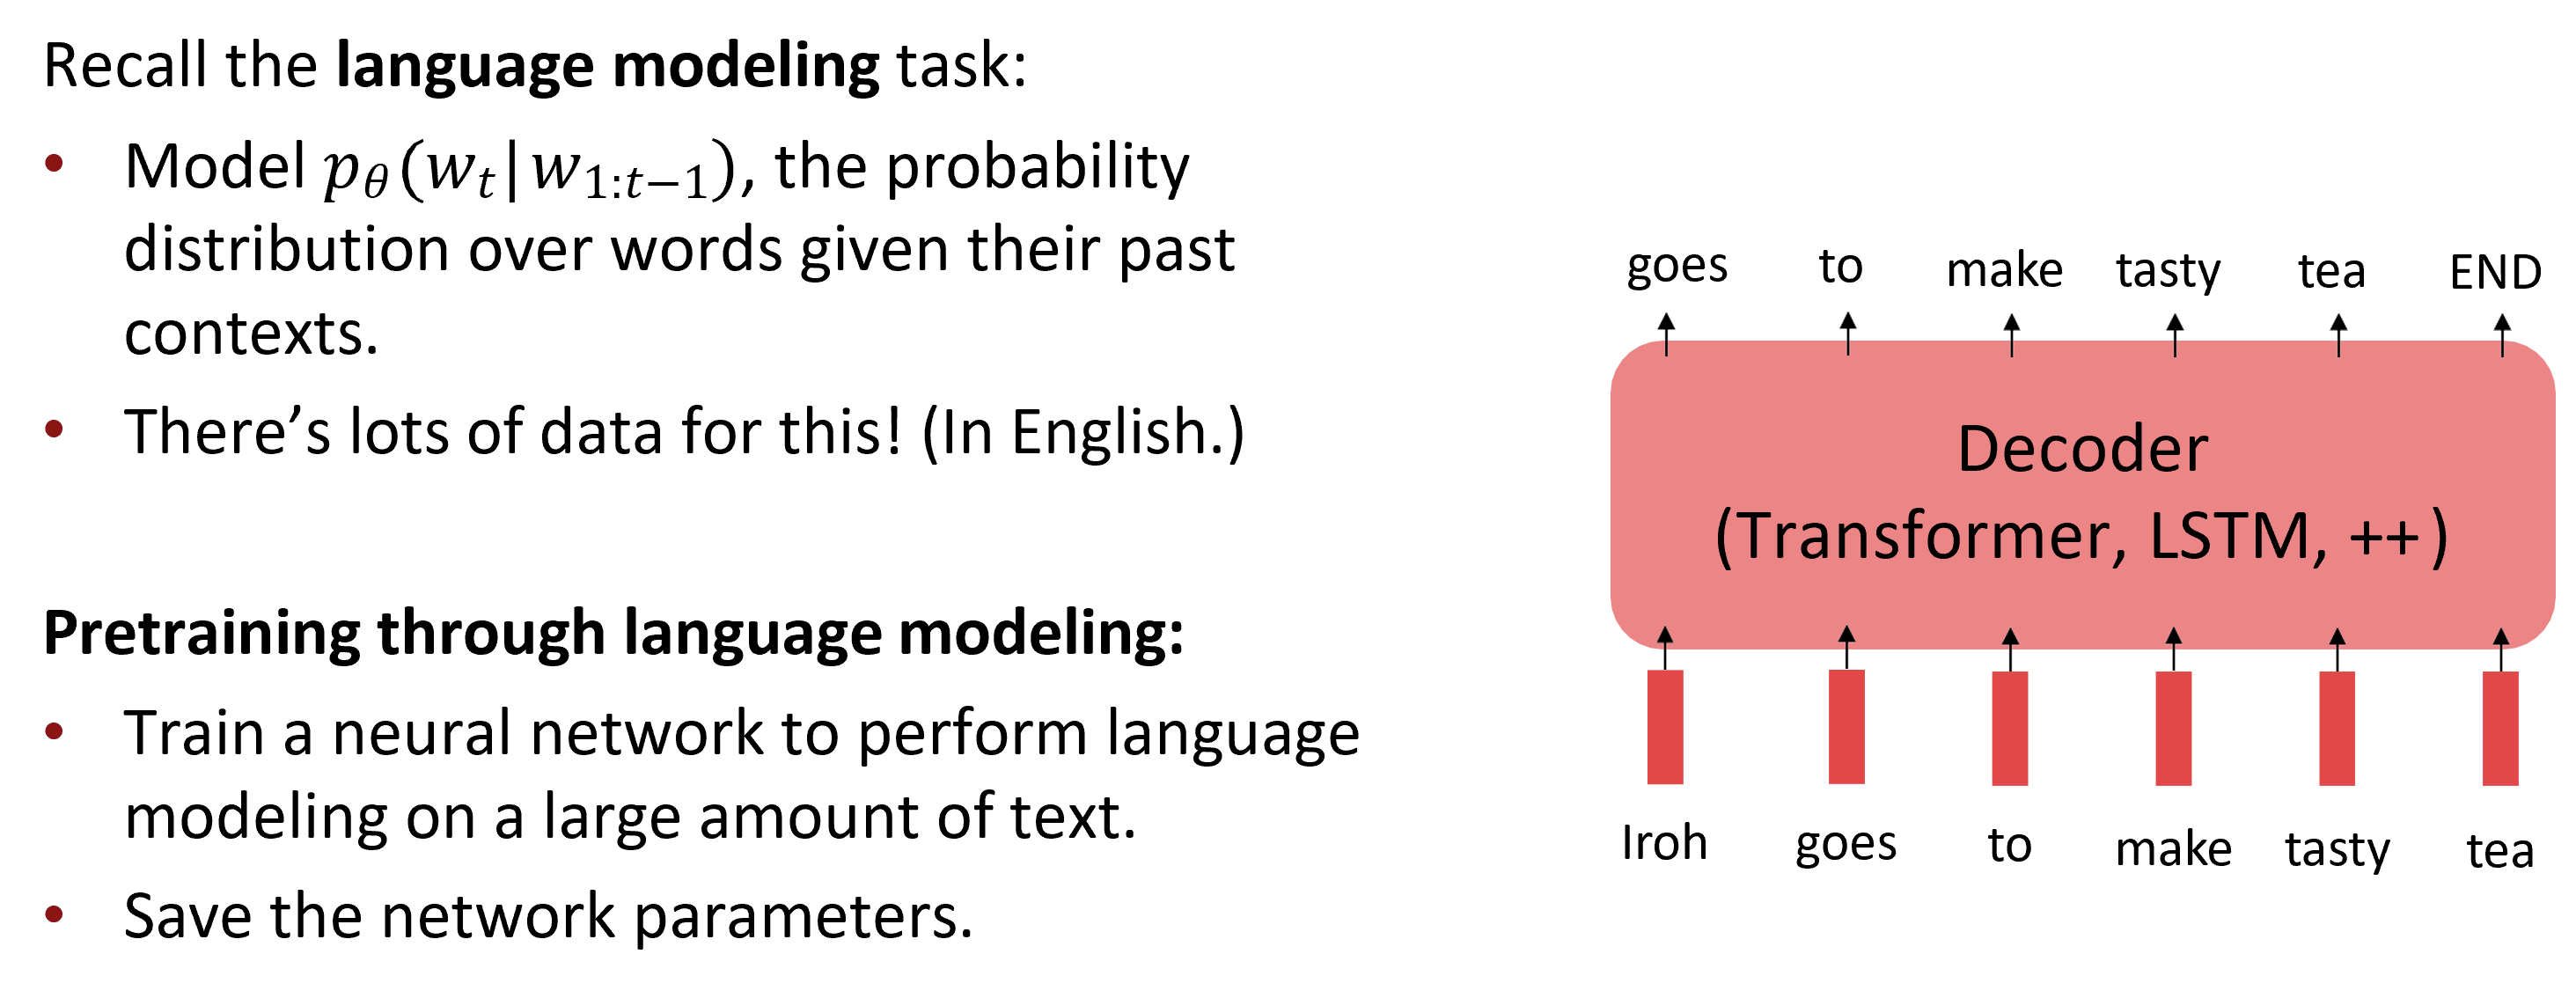
\includegraphics[width=\linewidth,keepaspectratio]{bert97}
			% \end{center}		
			
			% % {\tiny (Ref: John Hewitt)}

% \end{frame}

% %%%%%%%%%%%%%%%%%%%%%%%%%%%%%%%%%%%%%%%%%%%%%%%%%%%%%%%%%%%
% \begin{frame}[fragile]\frametitle{The Pretraining / Finetuning Paradigm}

			
			% \begin{center}
			% 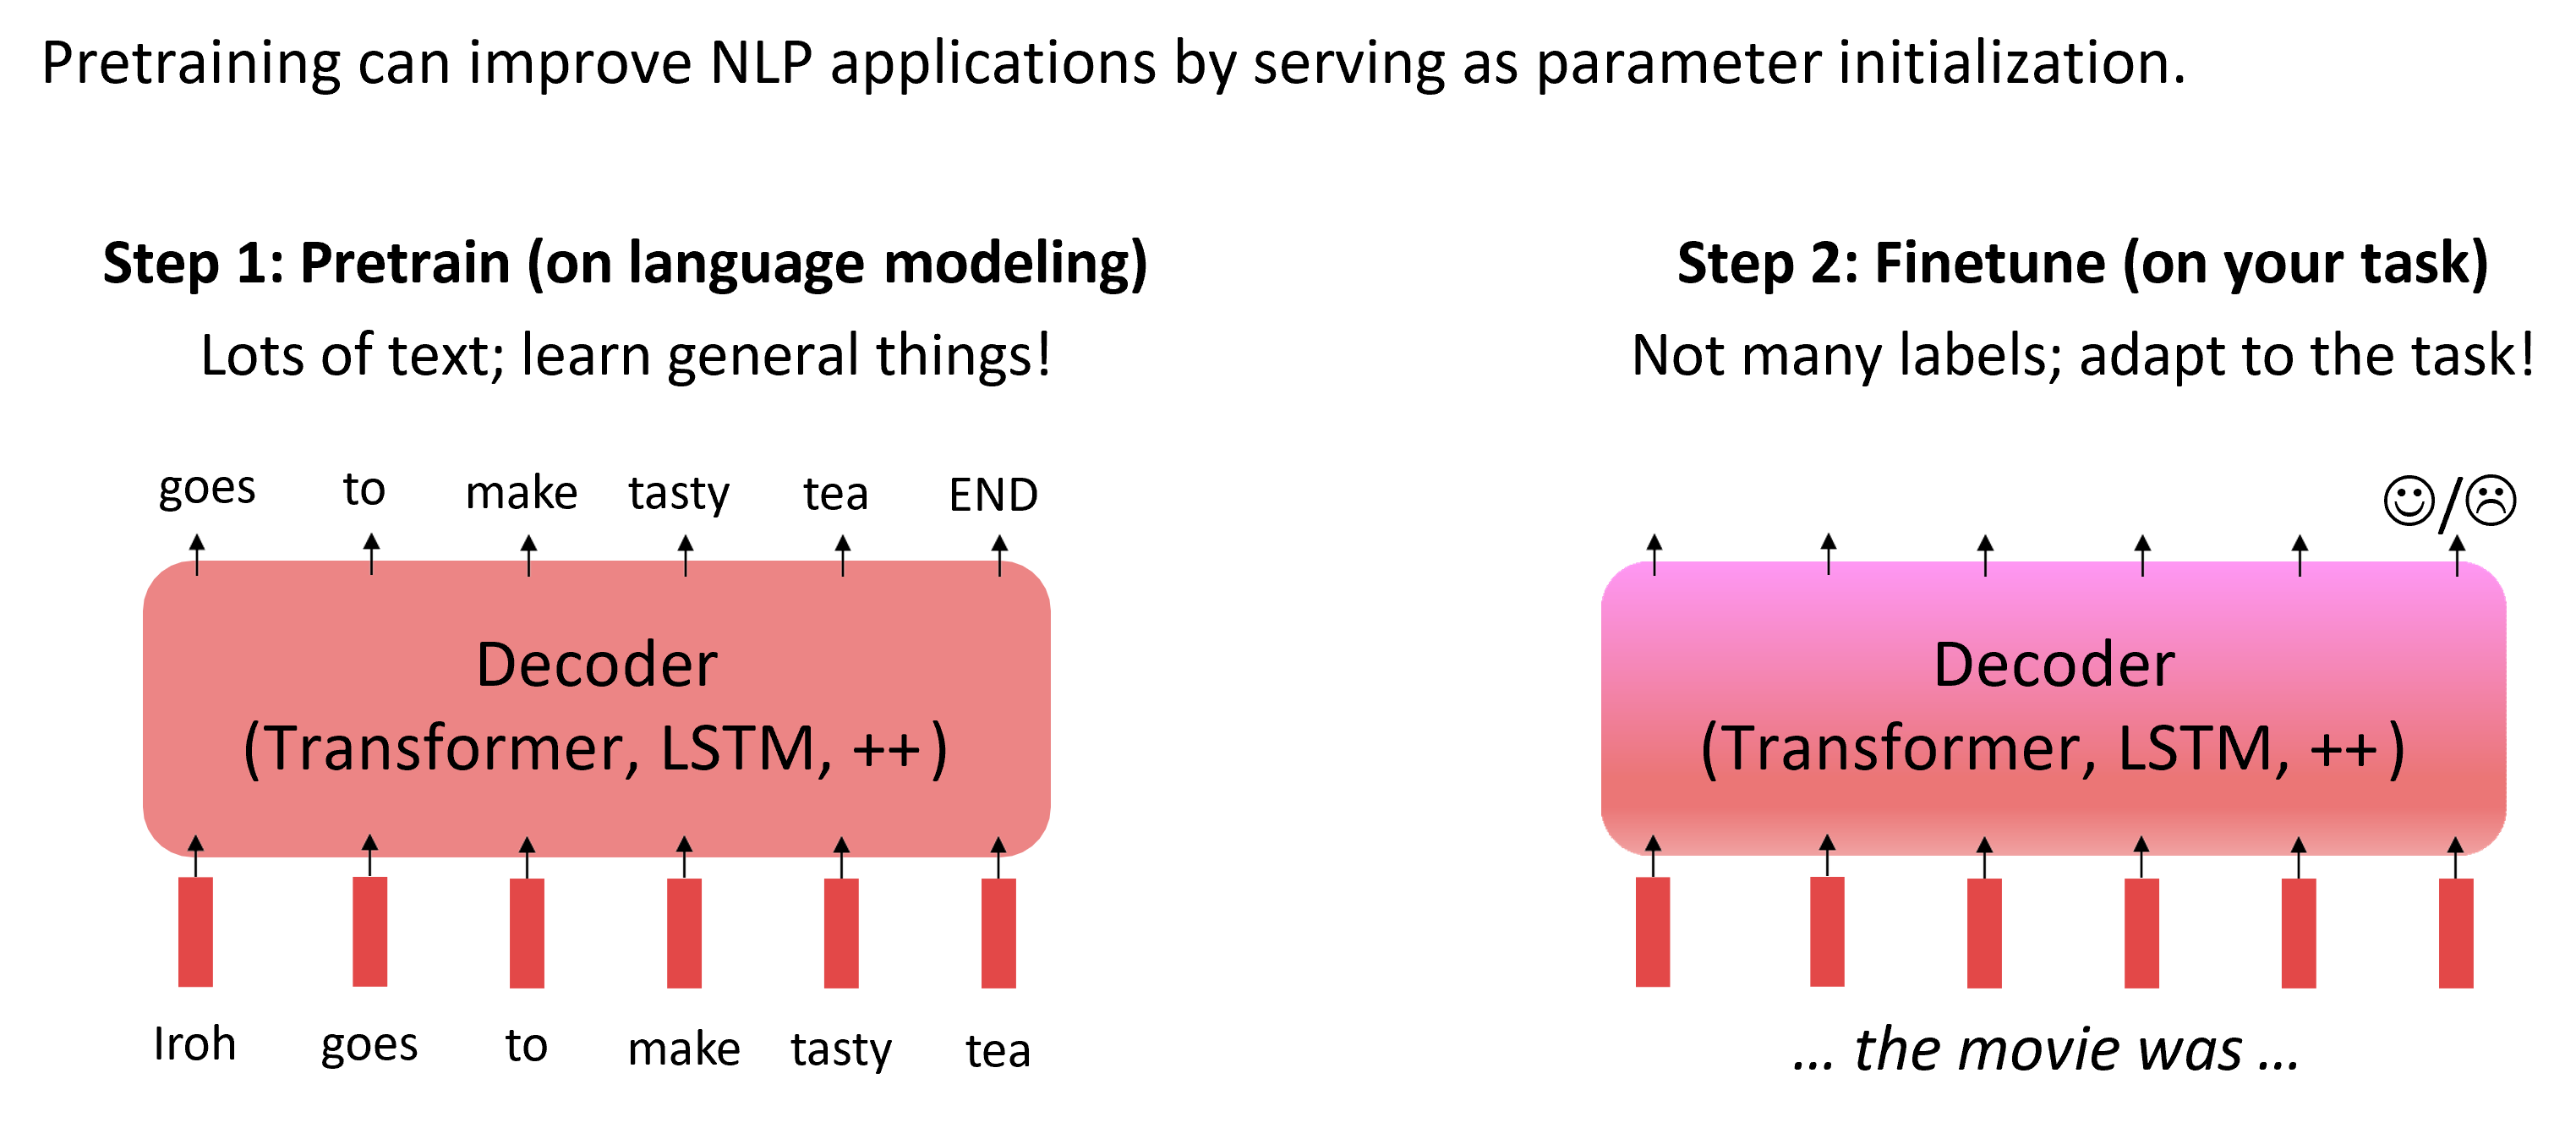
\includegraphics[width=\linewidth,keepaspectratio]{bert98}
			% \end{center}		
			
			% % {\tiny (Ref: John Hewitt)}

% \end{frame}

% % %%%%%%%%%%%%%%%%%%%%%%%%%%%%%%%%%%%%%%%%%%%%%%%%%%%%%%%%%%%
% % \begin{frame}[fragile]\frametitle{Capturing meaning via context}

% % Increasing evidence that pretrained models learn a wide variety of things about
% % the statistical properties of language:

      % % \begin{itemize}
			% % \item Stanford University is located in $--$, California. [Trivia]
			% % \item I put $--$ fork down on the table. [syntax]
			% % \item The woman walked across the street, checking for traffic over $--$ shoulder. [coreference]
			% % \item I went to the ocean to see the fish, turtles, seals, and $--$.	[lexical semantics/topic]
			% % \item Overall, the value I got from the two hours watching it was the sum total of the popcorn and the drink. The movie was $--$. [sentiment]
			% % \item Iroh went into the kitchen to make some tea. Standing next to Iroh, Zuko pondered his  destiny. Zuko left the $--$. [some reasoning – this is harder]
			% % \item I was thinking about the sequence that goes 1, 1, 2, 3, 5, 8, 13, 21, $--$[some basic arithmetic; they don’t learn the Fibonnaci sequence]
			% % \item Models also learn – and can exacerbate racism, sexism, all manner of bad biases.
			% % \item More on all this in the Interpretability lecture!

			% % \end{itemize}

			% % % {\tiny (Ref: John Hewitt)}

% % \end{frame}

% %%%%%%%%%%%%%%%%%%%%%%%%%%%%%%%%%%%%%%%%%%%%%%%%%%%%%%%%%%%
% \begin{frame}[fragile]\frametitle{Pretraining}

			% Pretraining for three types of architectures
			
			% \begin{center}
			% 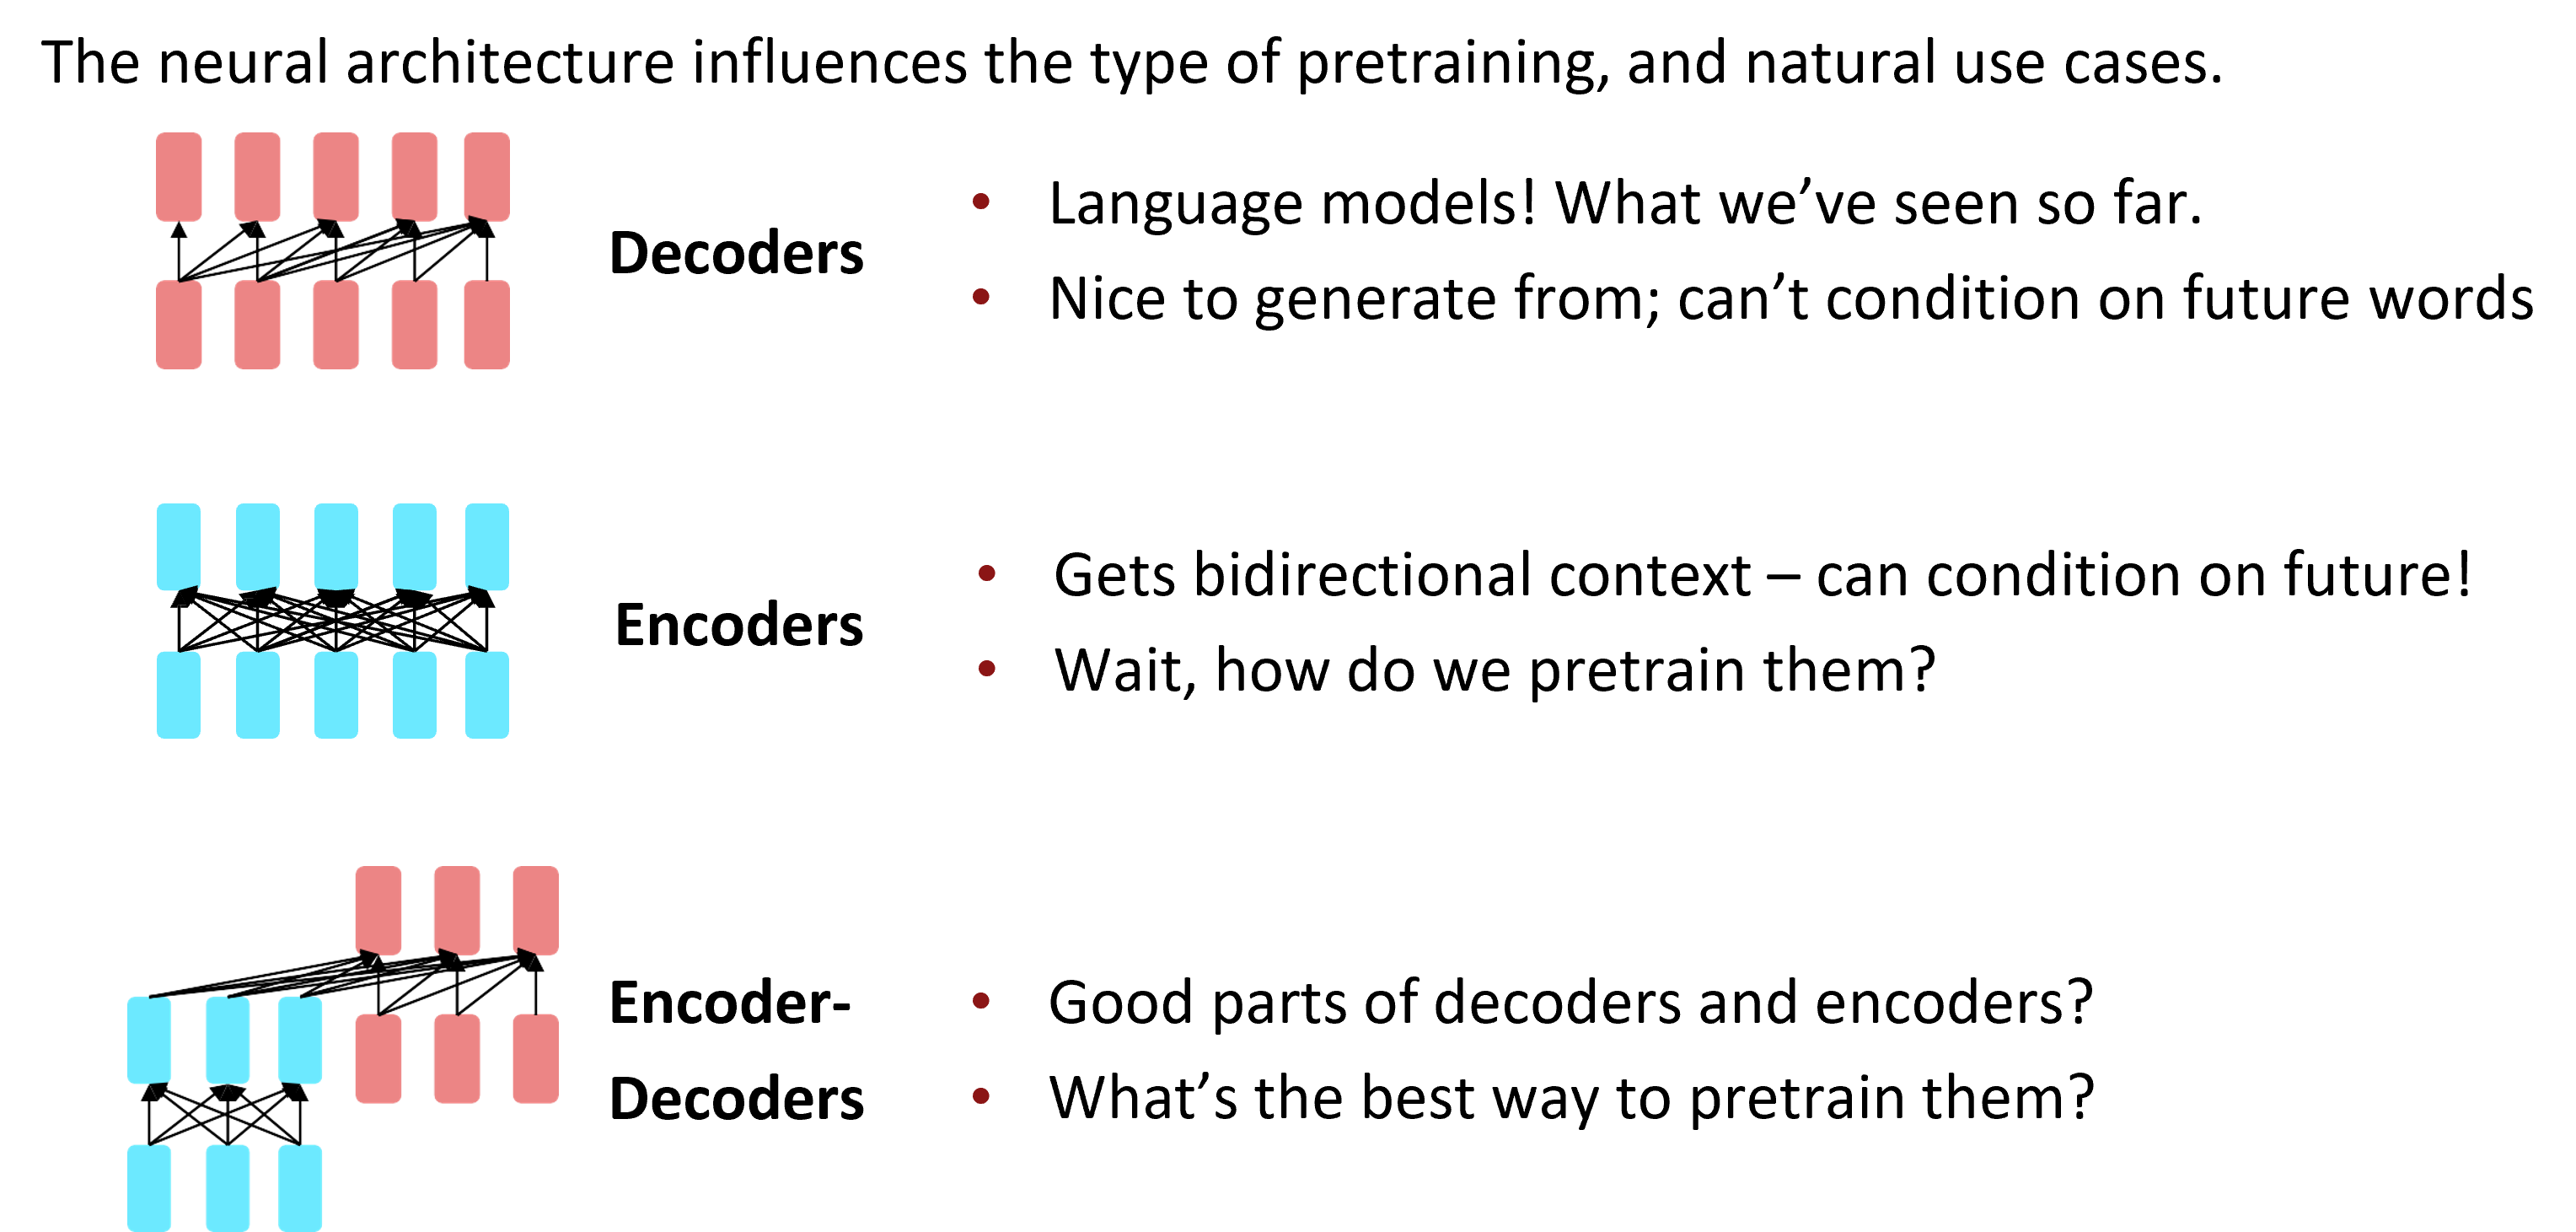
\includegraphics[width=\linewidth,keepaspectratio]{bert99}
			% \end{center}		
			
			% % {\tiny (Ref: John Hewitt)}

% \end{frame}

% %%%%%%%%%%%%%%%%%%%%%%%%%%%%%%%%%%%%%%%%%%%%%%%%%%%%%%%%%%%
% \begin{frame}[fragile]\frametitle{Pretraining}

			% Pretraining encoder-decoders: What pretraining objective to use?
			
			% \begin{center}
			% 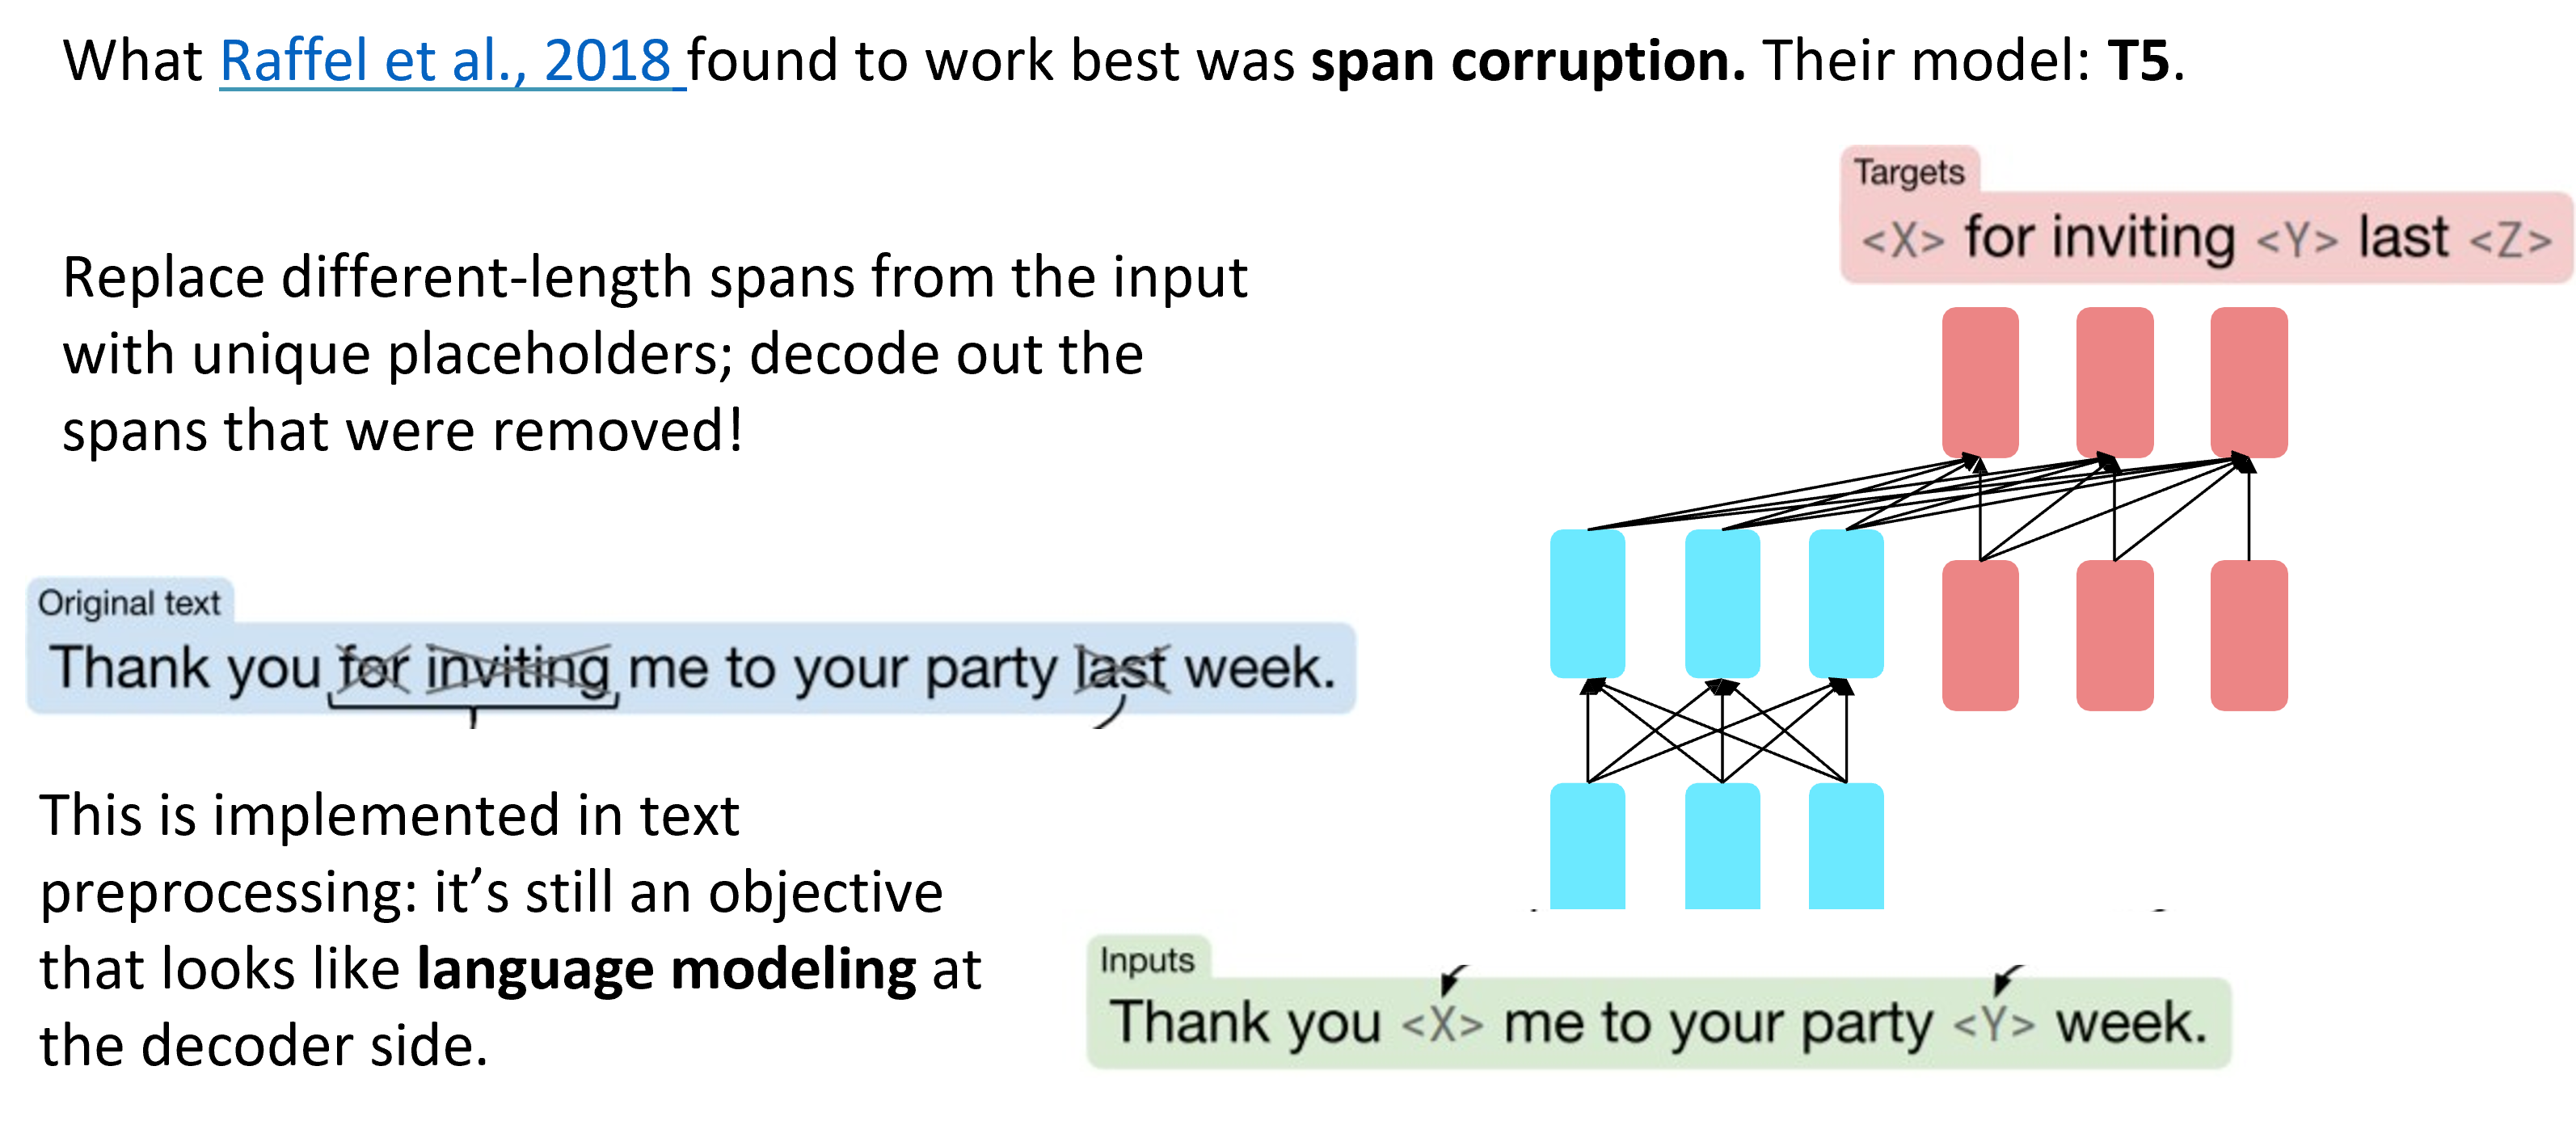
\includegraphics[width=\linewidth,keepaspectratio]{bert100}
			% \end{center}		
			
			% % {\tiny (Ref: John Hewitt)}

% \end{frame}

% %%%%%%%%%%%%%%%%%%%%%%%%%%%%%%%%%%%%%%%%%%%%%%%%%%%%%%%%%%%
% \begin{frame}[fragile]\frametitle{Pretraining}

			% Pretraining encoder-decoders: What pretraining objective to use?

			
			% \begin{center}
			% 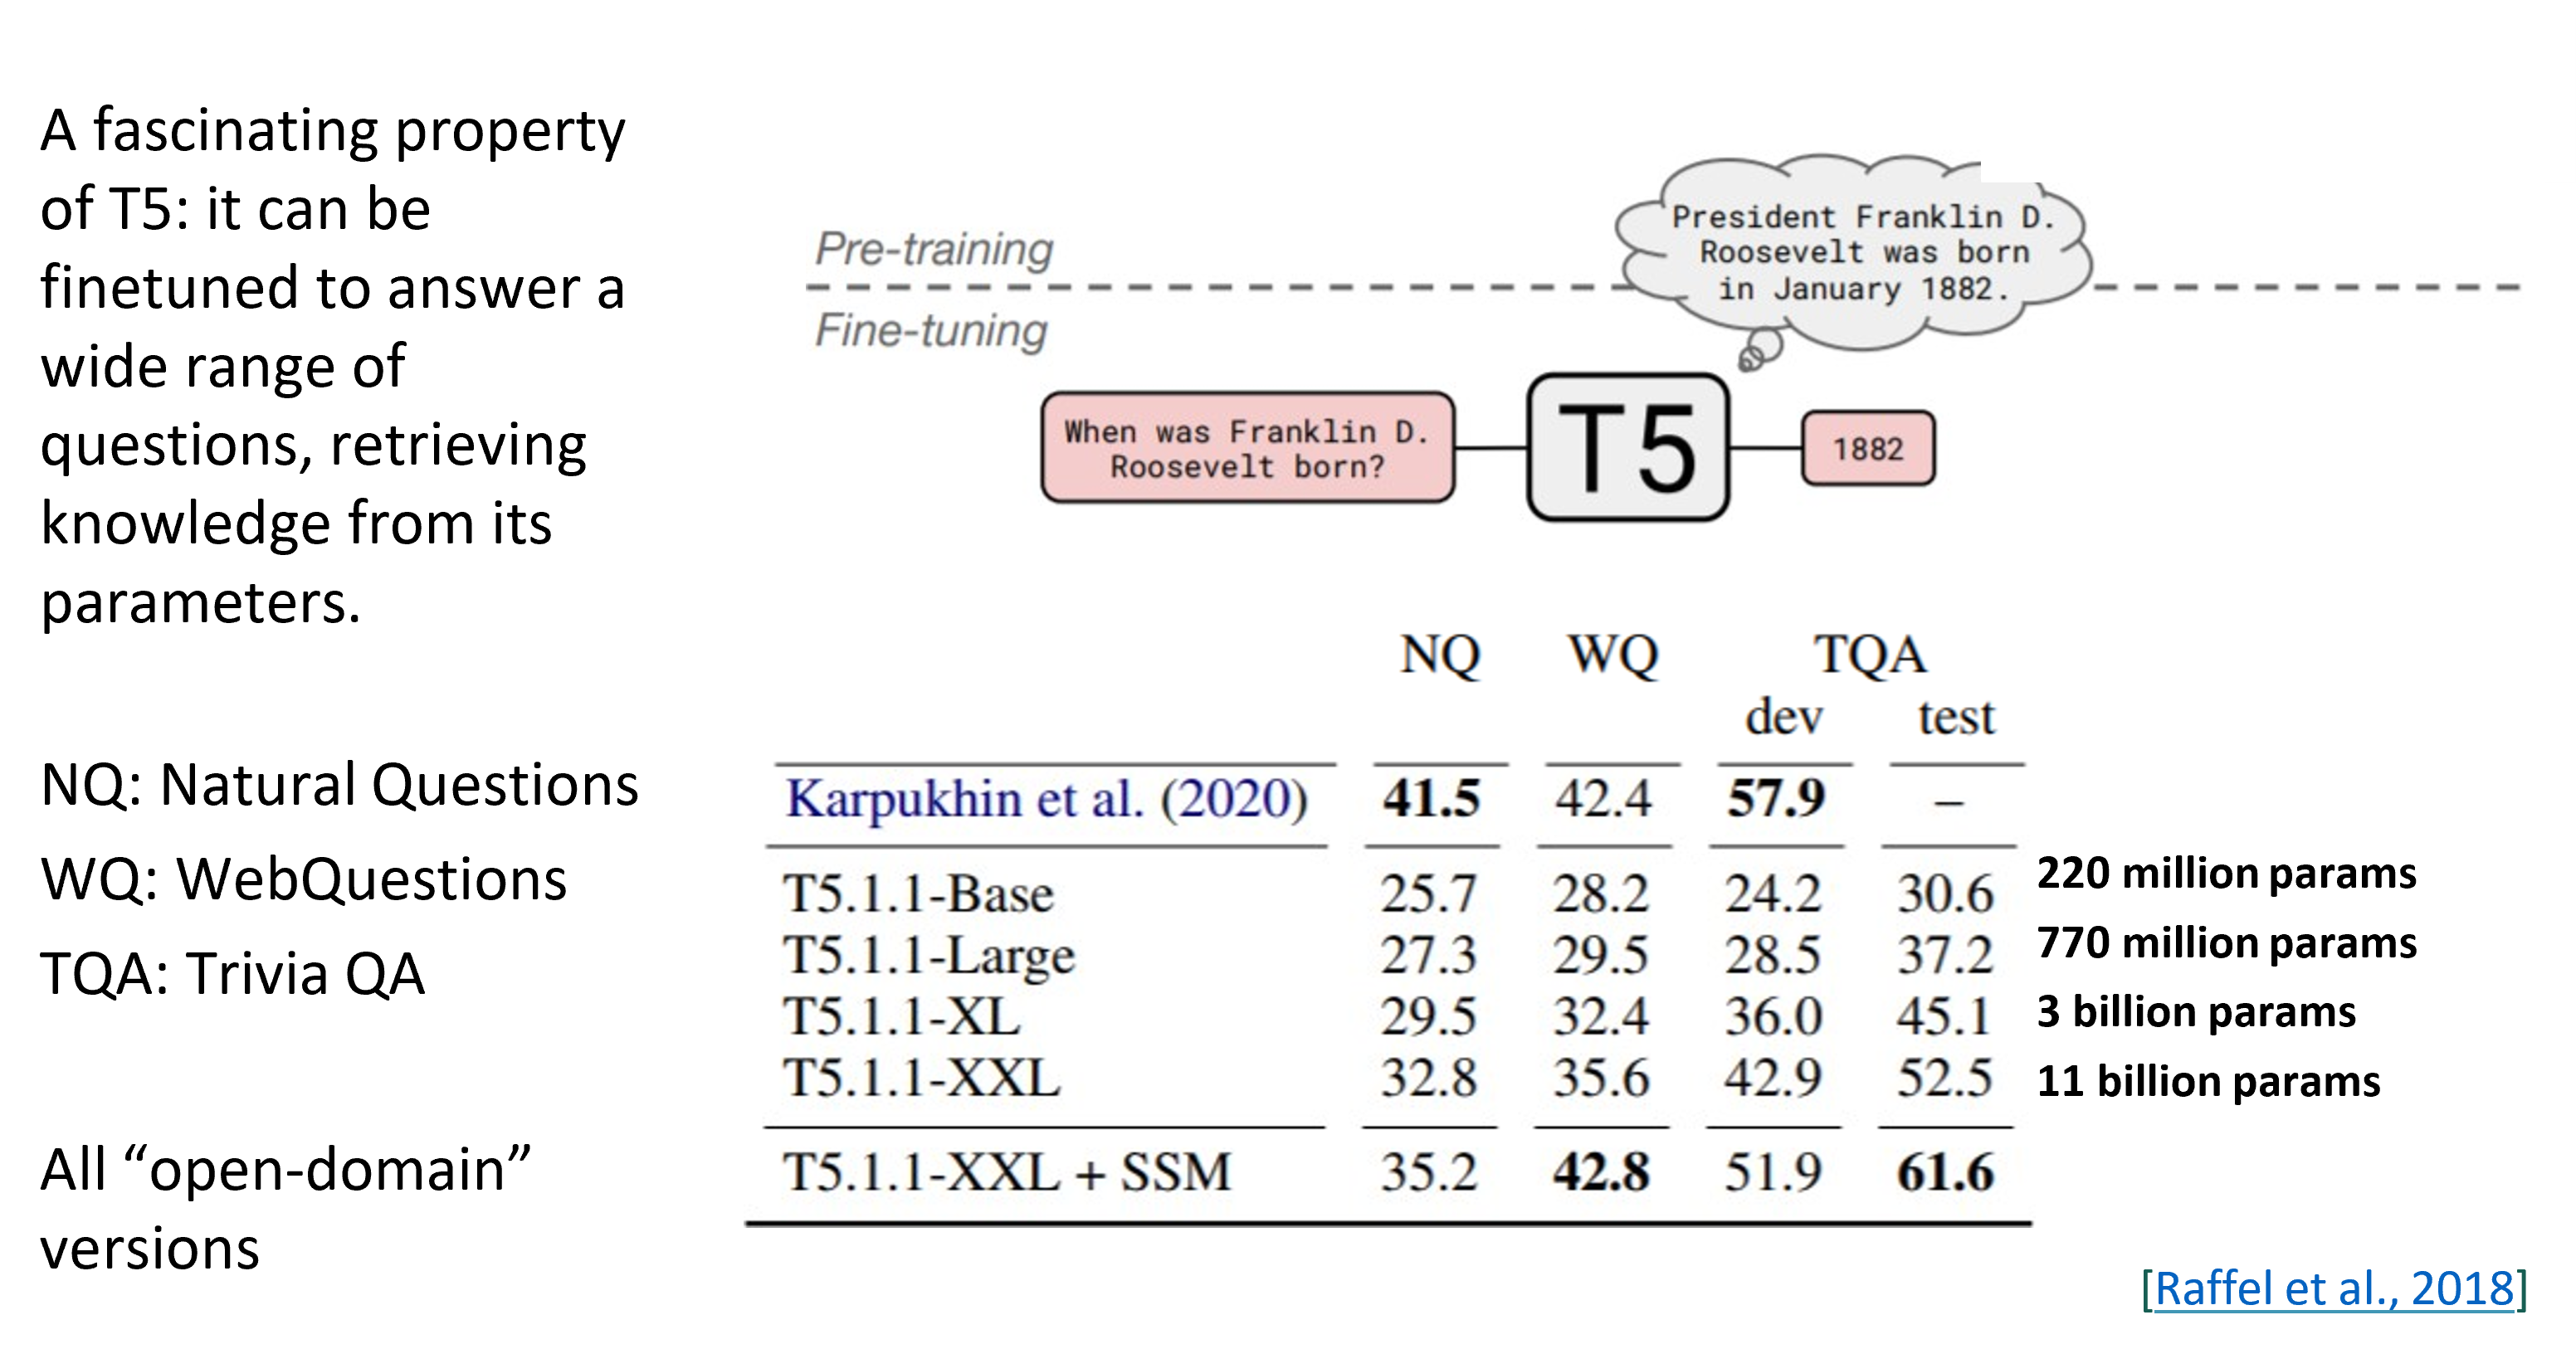
\includegraphics[width=\linewidth,keepaspectratio]{bert101}
			% \end{center}		
			
			% % {\tiny (Ref: John Hewitt)}

% \end{frame}


% %%%%%%%%%%%%%%%%%%%%%%%%%%%%%%%%%%%%%%%%%%%%%%%%%%%%%%%%%%%
% \begin{frame}[fragile]\frametitle{Pretraining decoders}


			% \begin{center}
			% 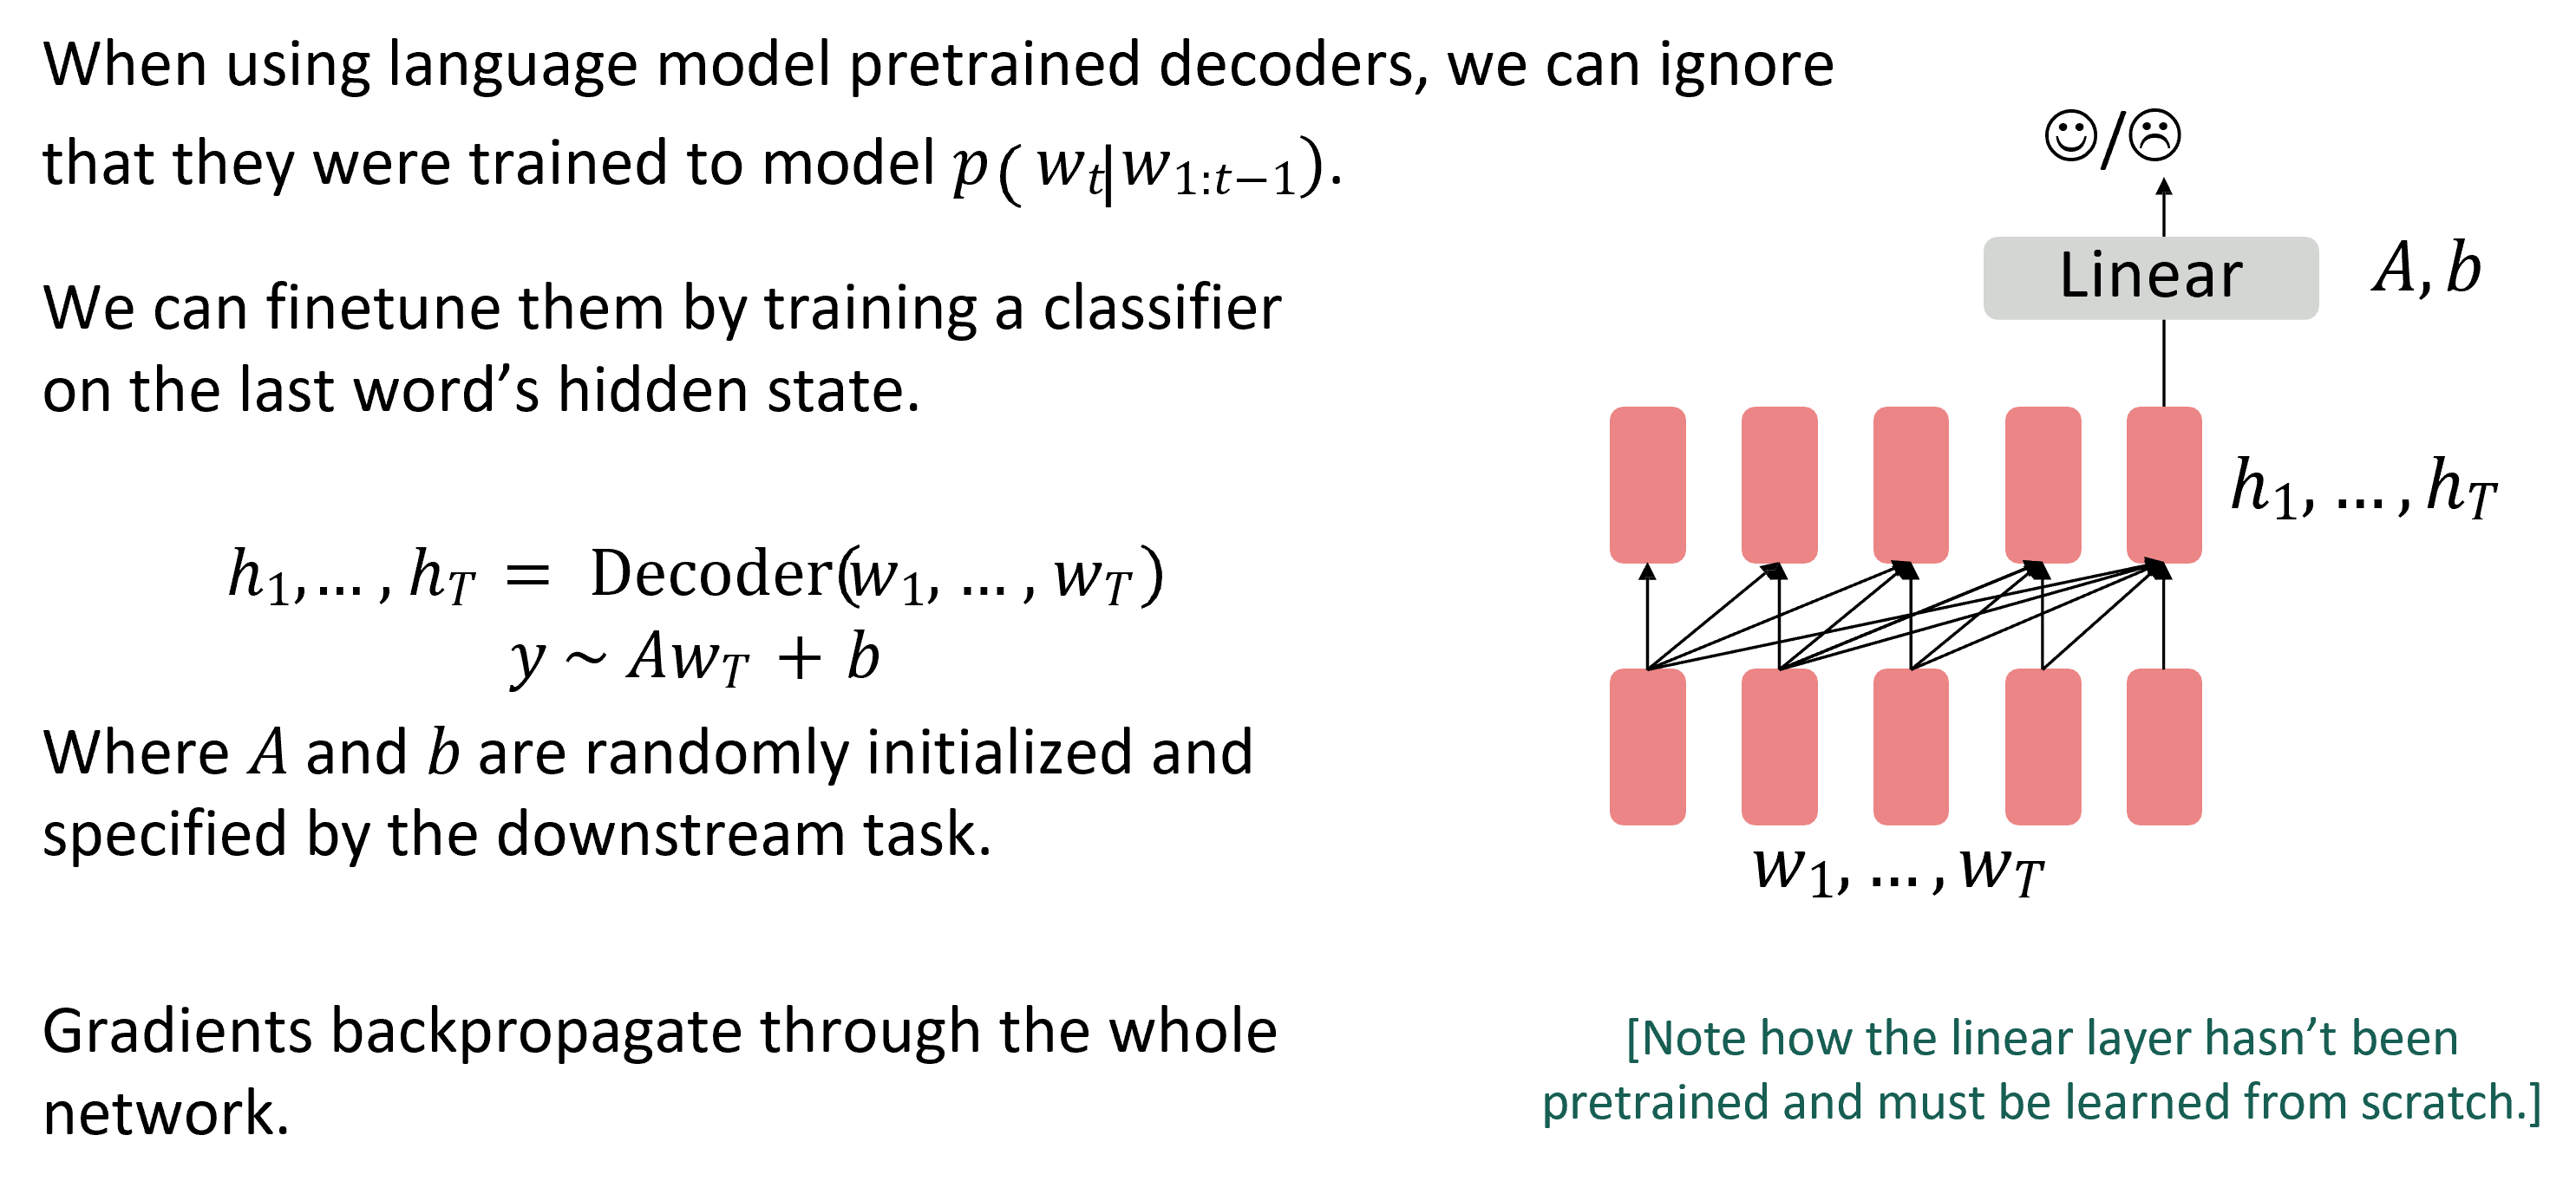
\includegraphics[width=\linewidth,keepaspectratio]{bert104}
			% \end{center}		
			
			% % {\tiny (Ref: John Hewitt)}

% \end{frame}

% %%%%%%%%%%%%%%%%%%%%%%%%%%%%%%%%%%%%%%%%%%%%%%%%%%%%%%%%%%%
% \begin{frame}[fragile]\frametitle{Pretraining decoders}


			% \begin{center}
			% 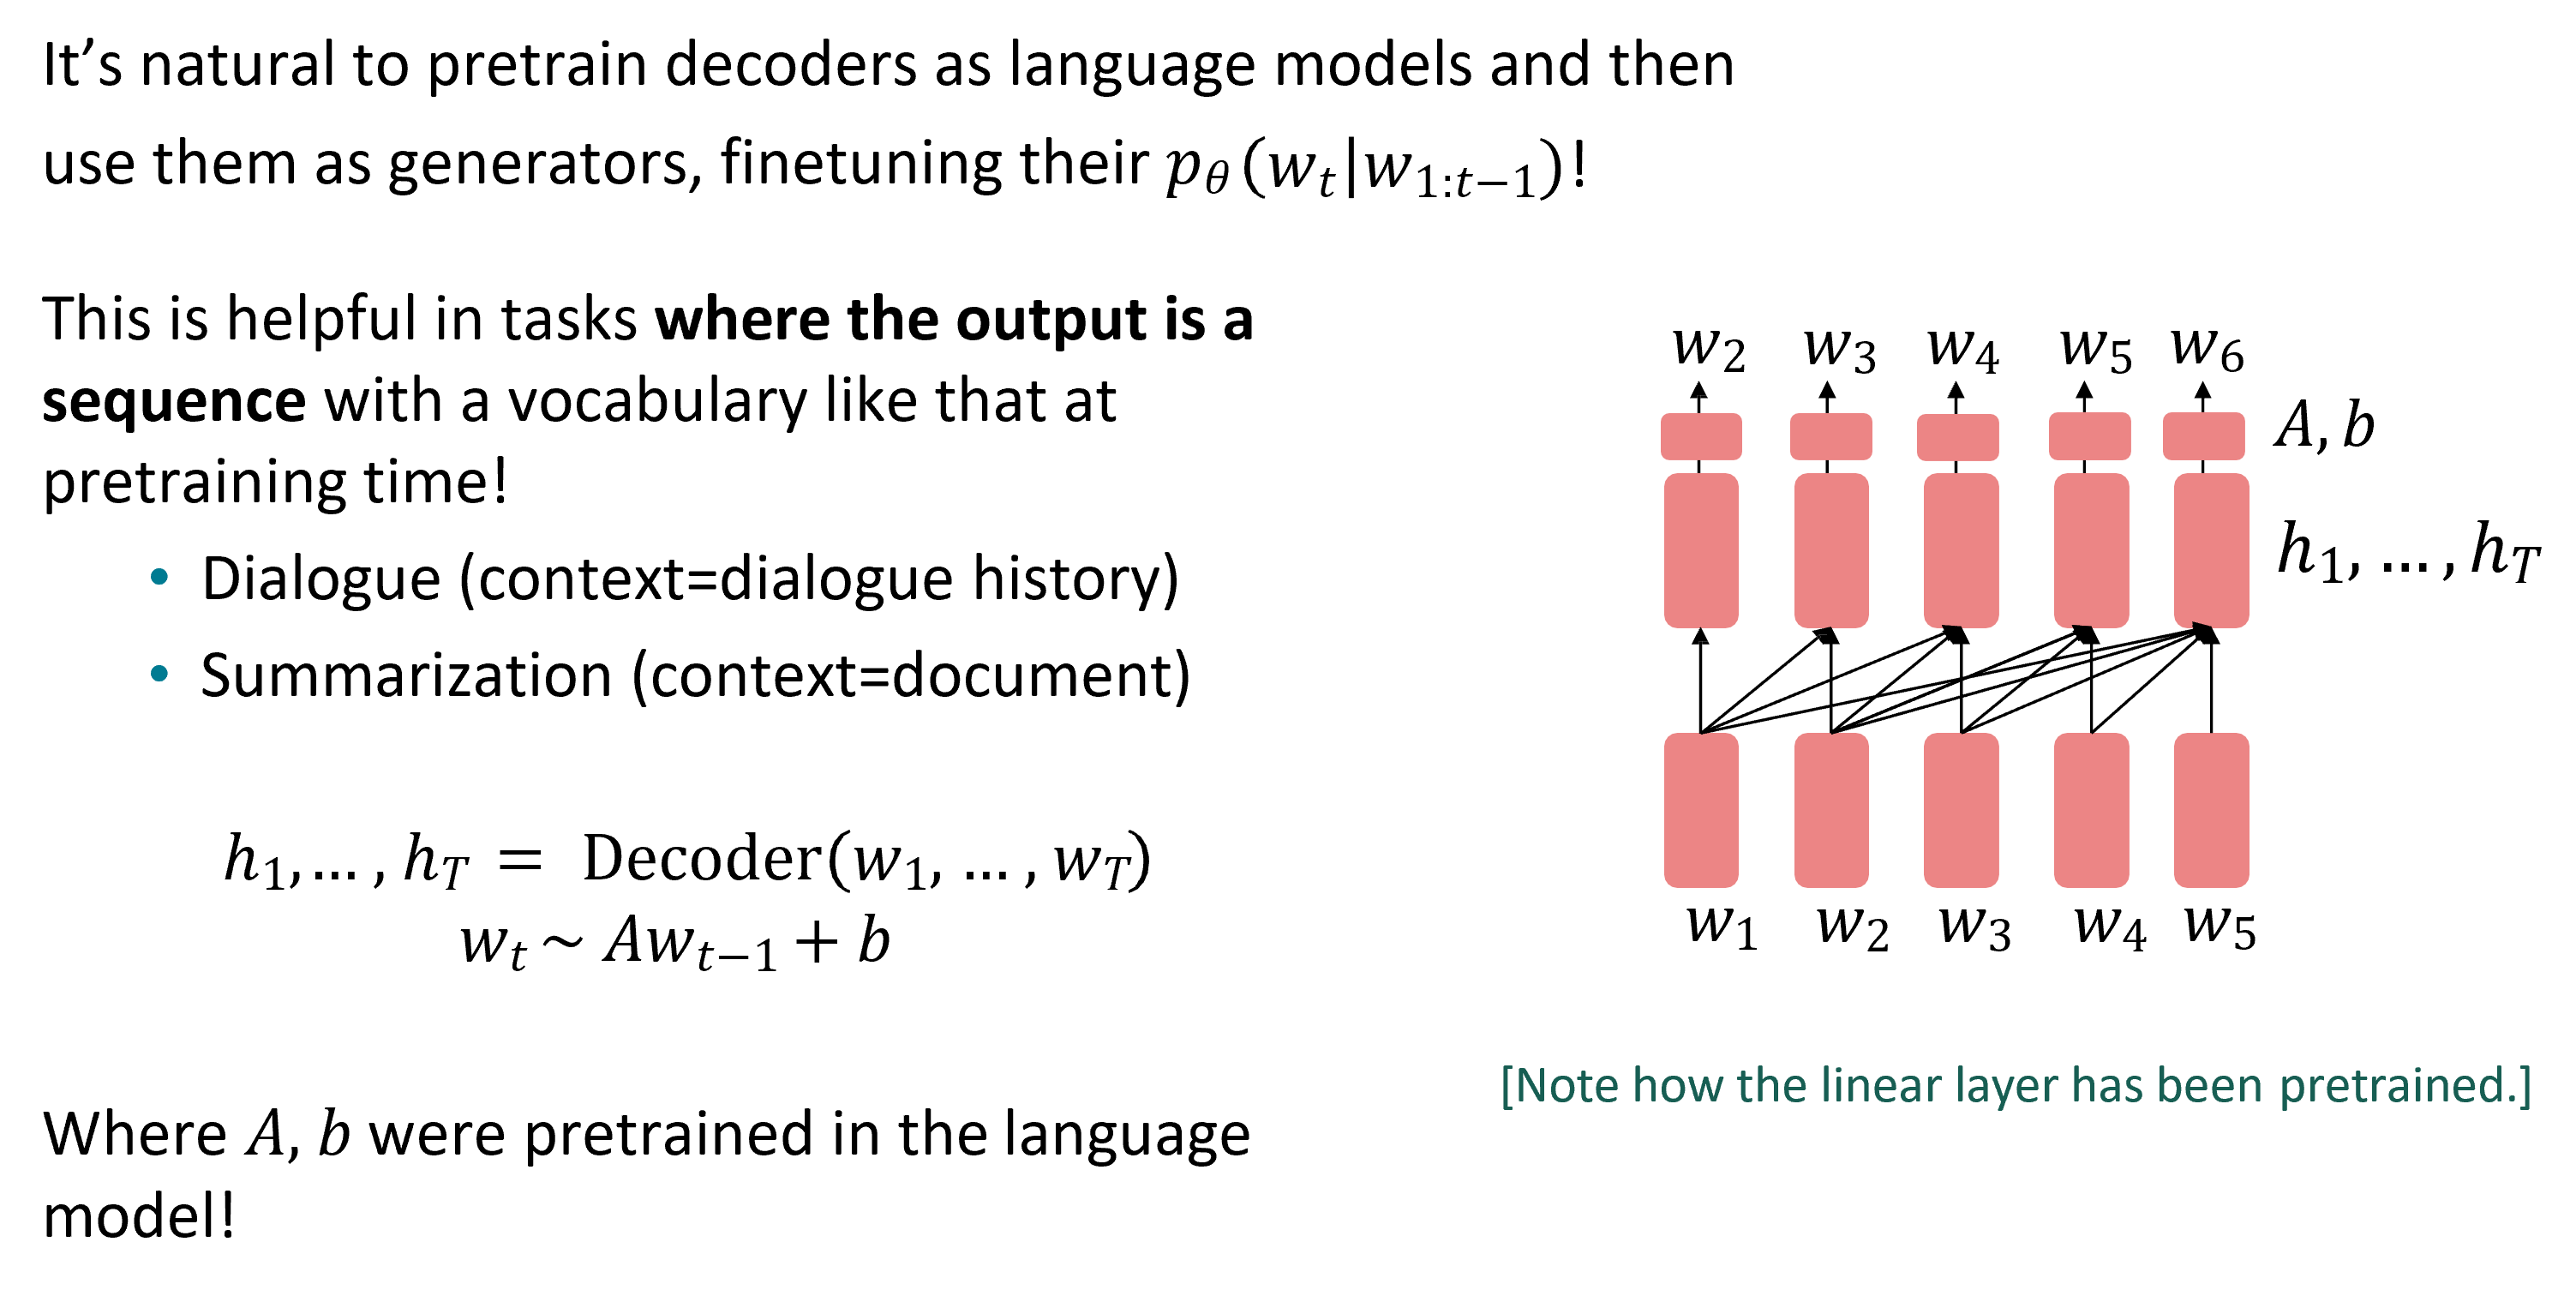
\includegraphics[width=\linewidth,keepaspectratio]{bert105}
			% \end{center}		
			
			% % {\tiny (Ref: John Hewitt)}

% \end{frame}

% % %%%%%%%%%%%%%%%%%%%%%%%%%%%%%%%%%%%%%%%%%%%%%%%%%%%%%%%%%%%
% % \begin{frame}[fragile]\frametitle{Aside: Word structure and subword models}

			% % \begin{center}
			% % 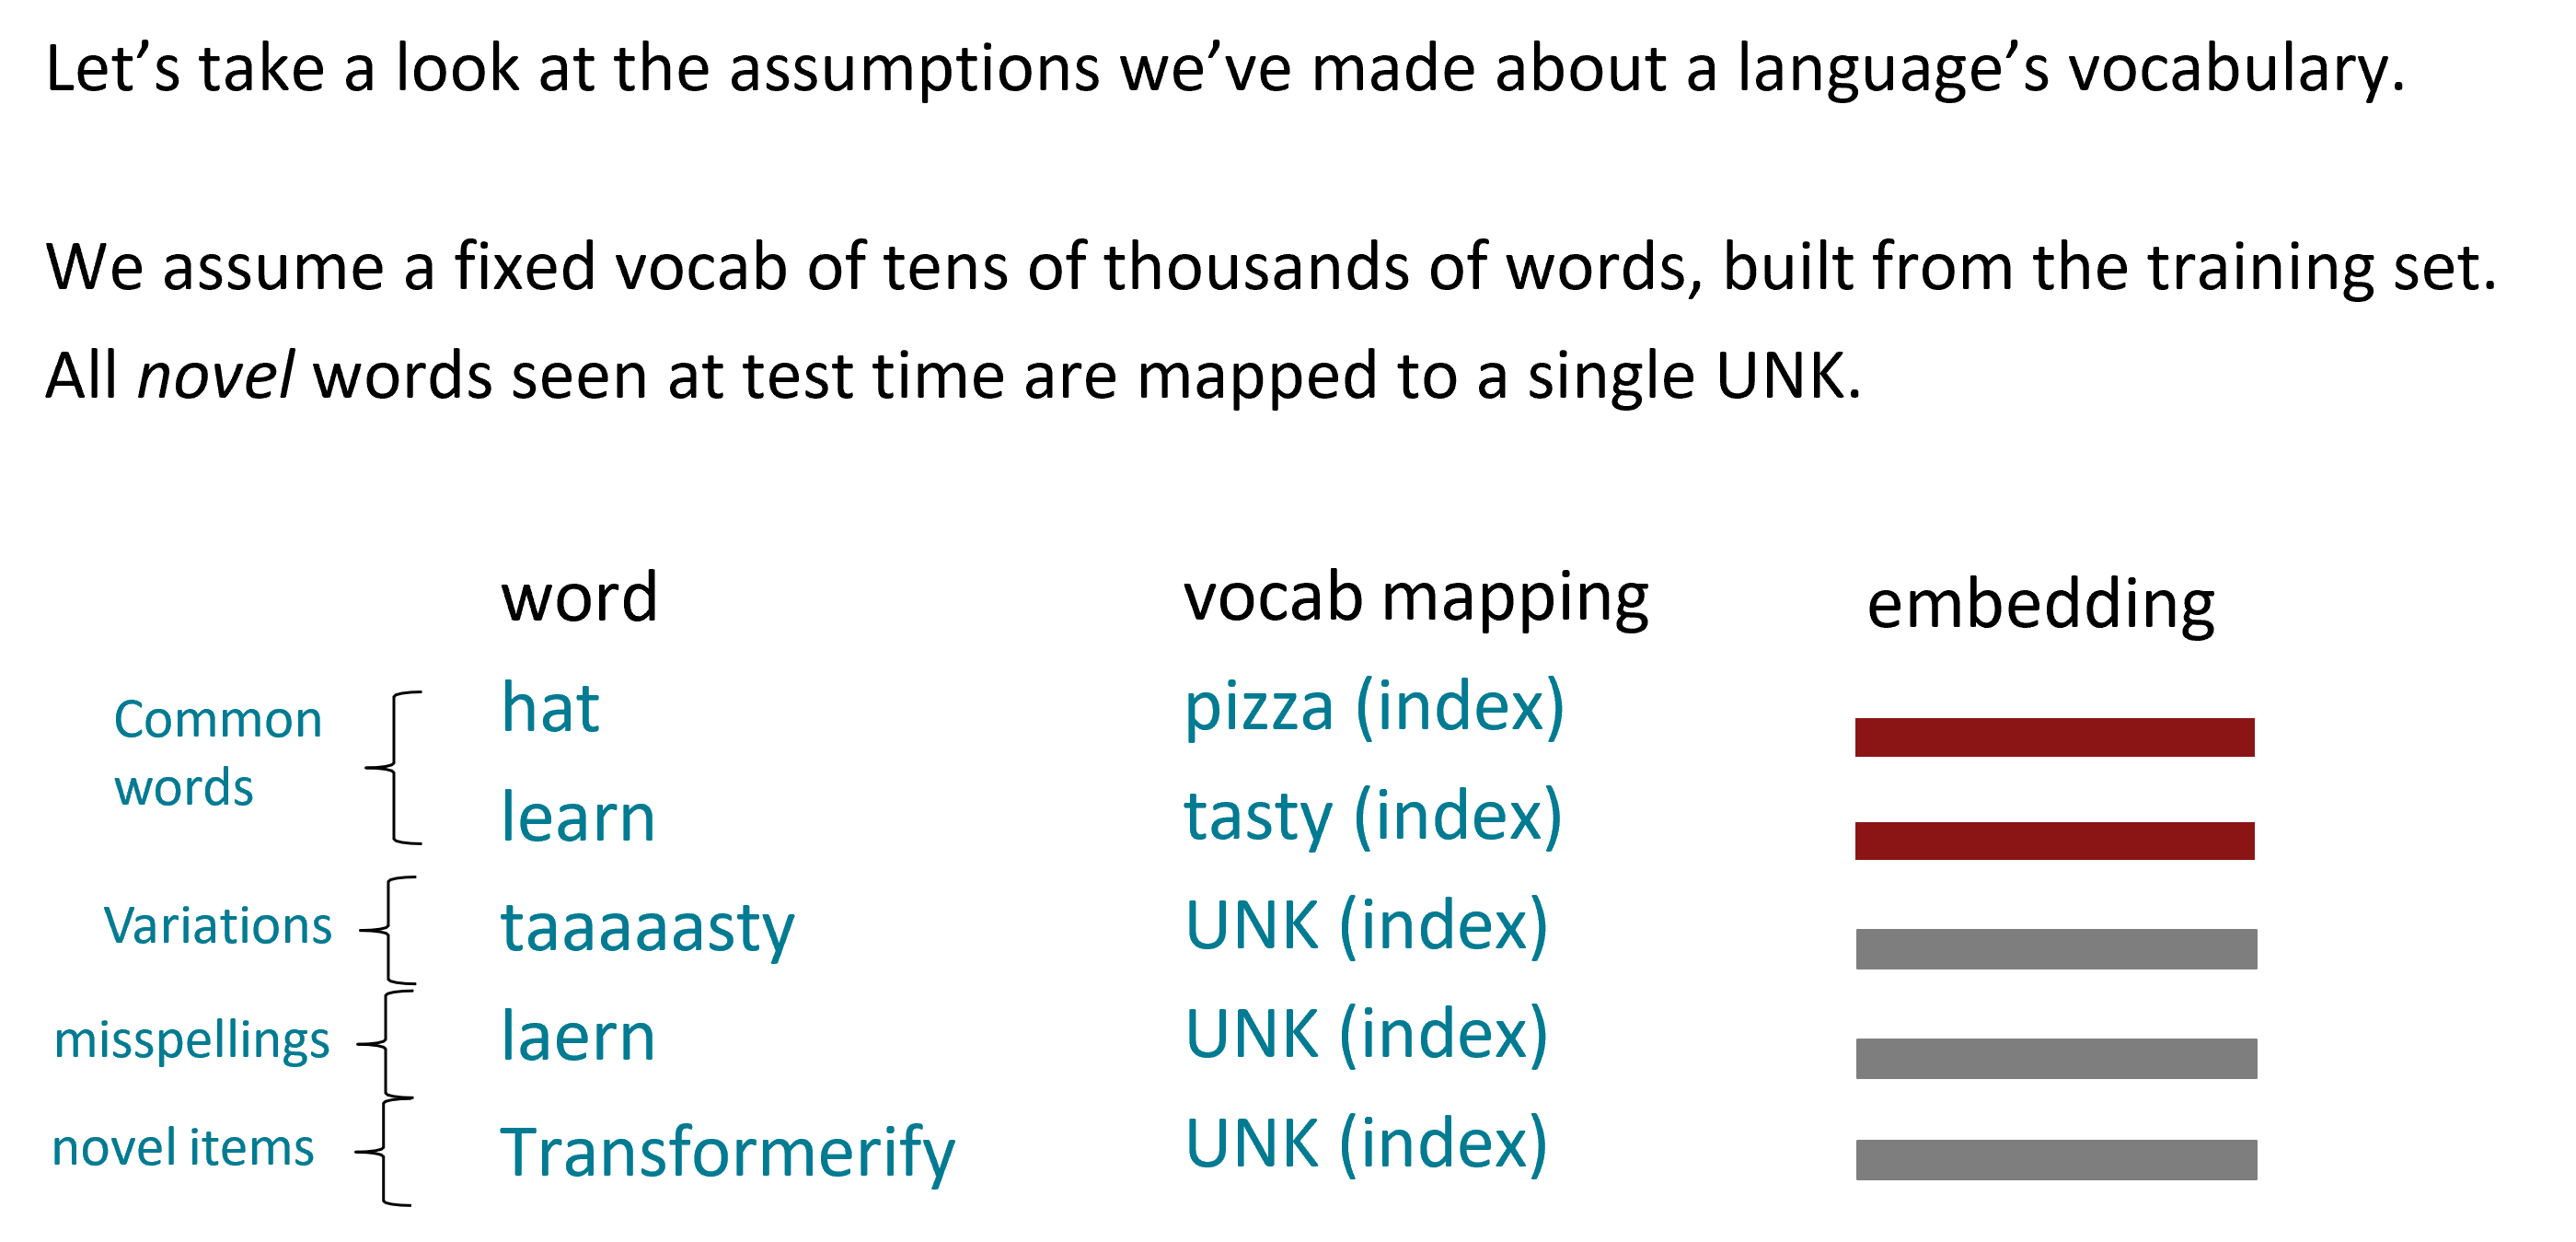
\includegraphics[width=\linewidth,keepaspectratio]{bert109}
			% % \end{center}		
			
			% % % {\tiny (Ref: John Hewitt)}

% % \end{frame}

% % %%%%%%%%%%%%%%%%%%%%%%%%%%%%%%%%%%%%%%%%%%%%%%%%%%%%%%%%%%%
% % \begin{frame}[fragile]\frametitle{Aside: Word structure and subword models}

			% % \begin{center}
			% % \includegraphics[width=\linewidth,keepaspectratio]{bert110}
			% % \end{center}		
			
			% % % {\tiny (Ref: John Hewitt)}

% % \end{frame}


% % %%%%%%%%%%%%%%%%%%%%%%%%%%%%%%%%%%%%%%%%%%%%%%%%%%%%%%%%%%%
% % \begin{frame}[fragile]\frametitle{Aside: The byte-pair encoding algorithm}

			% % \begin{center}
			% % \includegraphics[width=\linewidth,keepaspectratio]{bert111}
			% % \end{center}		
			
			% % % {\tiny (Ref: John Hewitt)}

% % \end{frame}

% % %%%%%%%%%%%%%%%%%%%%%%%%%%%%%%%%%%%%%%%%%%%%%%%%%%%%%%%%%%%
% % \begin{frame}[fragile]\frametitle{Aside: Word structure and subword models}

			% % \begin{center}
			% % \includegraphics[width=\linewidth,keepaspectratio]{bert112}
			% % \end{center}		
			
			% % % {\tiny (Ref: John Hewitt)}

% % \end{frame}

% %%%%%%%%%%%%%%%%%%%%%%%%%%%%%%%%%%%%%%%%%%%%%%%%%%%%%%%%%%%%%%%%%%%%%%%%%%%%%%%%%%
% \begin{frame}[fragile]\frametitle{}
% \begin{center}
% {\Large GPT}
% \end{center}
% \end{frame}


% %%%%%%%%%%%%%%%%%%%%%%%%%%%%%%%%%%%%%%%%%%%%%%%%%%%%%%%%%%%
% \begin{frame}[fragile]\frametitle{Generative Pretrained Transformer (GPT)}

% [Radford et al., 2018]

% 2018’s GPT was a big success in pretraining a decoder!


      % \begin{itemize}
			% \item Transformer decoder with 12 layers.
			% \item 768-dimensional hidden states, 3072-dimensional feed-forward hidden layers.
			% \item Byte-pair encoding with 40,000 merges
			% \item Trained on BooksCorpus: over 7000 unique books.
			% \item Contains long spans of contiguous text, for learning long-distance dependencies.
			% \item The acronym ``GPT'' never showed up in the original paper; it could stand for
			% \item ``Generative PreTraining'' or ``Generative Pretrained Transformer''
			% \end{itemize}

			
			% % {\tiny (Ref: John Hewitt)}

% \end{frame}

% %%%%%%%%%%%%%%%%%%%%%%%%%%%%%%%%%%%%%%%%%%%%%%%%%%%%%%%%%%%
% \begin{frame}[fragile]\frametitle{GPT}

			% \begin{center}
			% \includegraphics[width=\linewidth,keepaspectratio]{bert106}
			% \end{center}		
			
			% % {\tiny (Ref: John Hewitt)}

% \end{frame}

% %%%%%%%%%%%%%%%%%%%%%%%%%%%%%%%%%%%%%%%%%%%%%%%%%%%%%%%%%%%
% \begin{frame}[fragile]\frametitle{GPT}

			% \begin{center}
			% \includegraphics[width=\linewidth,keepaspectratio]{bert107}
			% \end{center}		
			
			% % {\tiny (Ref: John Hewitt)}

% \end{frame}

% %%%%%%%%%%%%%%%%%%%%%%%%%%%%%%%%%%%%%%%%%%%%%%%%%%%%%%%%%%%
% \begin{frame}[fragile]\frametitle{GPT}

			% \begin{center}
			% \includegraphics[width=\linewidth,keepaspectratio]{bert108}
			% \end{center}		
			
			% % {\tiny (Ref: John Hewitt)}

% \end{frame}



% %%%%%%%%%%%%%%%%%%%%%%%%%%%%%%%%%%%%%%%%%%%%%%%%%%%%%%%%%%%
% \begin{frame}[fragile]\frametitle{GPT-3, in-context learning, very large models}


      % \begin{itemize}
			% \item So far, we’ve interacted with pretrained models in two ways:
			      % \begin{itemize}
						% \item Sample from the distributions they define (maybe providing a prompt)
						% \item Fine-tune them on a task we care about, and take their predictions.
						% \end{itemize}
			% \item Very large language models seem to perform some kind of learning without gradient  steps simply from examples you provide within their contexts.
			% \item GPT-3 is the canonical example of this. The largest T5 model had 11 billion parameters.
			% \item GPT-3 has 175 billion parameters.

			% \end{itemize}

			% % {\tiny (Ref: John Hewitt)}

% \end{frame}

% %%%%%%%%%%%%%%%%%%%%%%%%%%%%%%%%%%%%%%%%%%%%%%%%%%%%%%%%%%%
% \begin{frame}[fragile]\frametitle{GPT-3, in-context learning, very large models}


      % \begin{itemize}
			% \item Very large language models seem to perform some kind of learning without gradient  steps simply from examples you provide within their contexts.
			% \item The in-context examples seem to specify the task to be performed, and the conditional  distribution mocks performing the task to a certain extent.
			% \item Input (prefix within a single Transformer decoder context):
			% \end{itemize}

			% \begin{center}
			% \includegraphics[width=0.4\linewidth,keepaspectratio]{bert102}
			% \end{center}		
			
			% % {\tiny (Ref: John Hewitt)}

% \end{frame}

% %%%%%%%%%%%%%%%%%%%%%%%%%%%%%%%%%%%%%%%%%%%%%%%%%%%%%%%%%%%
% \begin{frame}[fragile]\frametitle{GPT-3, in-context learning, very large models}


			% \begin{center}
			% \includegraphics[width=\linewidth,keepaspectratio]{bert103}
			% \end{center}		
			
			% % {\tiny (Ref: John Hewitt)}

% \end{frame}
